\documentclass[11pt]{article}

%\usepackage{palatino}

\usepackage[utf8]{inputenc}
\usepackage[T1]{fontenc}
% Chivo como en las diapositivas o Fira Sans?
%\usepackage[familydefault,regular]{Chivo}
\usepackage[sfdefault,scaled=.85]{FiraSans}
\usepackage{newtxsf}
\usepackage[spanish]{babel}
\setlength{\parindent}{0pt}
\usepackage{ amssymb }
\usepackage{amsmath}
\usepackage{ wasysym }
\usepackage{color}
\usepackage{graphics}
\usepackage{caption}
\usepackage{lipsum}
\usepackage{float}
\usepackage{adjustbox}
\usepackage{geometry}  

\geometry{left=3cm,right=3cm,top=3cm,bottom=3cm,headheight=1cm,headsep=0.5cm} 

\definecolor{text}{RGB}{78,78,78}
\definecolor{accent}{RGB}{129, 26, 24}


%%% PGFPLOTSTABLE

\usepackage{pgfplotstable}


\pgfplotstableset{
columns/0/.style={
     column name={Elementos},
   },
columns/1/.style={
     column name={Tiempo en segundos},
   },
}

\title{Algorítmica: práctica 1 \\ \large Análisis de la eficiencia de algoritmos}
\author{Sofía Almeida Bruno \and Antonio Coín Castro \and María Victoria Granados Pozo \and Miguel Lentisco Ballesteros \and José María Martín Luque}
\date{\today}

\begin{document}
\maketitle

\newpage

\section*{Introducción}
El objetivo de esta práctica es estudiar la eficiencia de los algoritmos que se nos proponen. Para ello realizaremos un estudio teórico, empírico e híbrido de cada uno de ellos. 
El estudio teórico consiste en expresar el número de operaciones $T(n)$ requeridas para un problema concreto en función del tamaño $n$, siempre en el \textit{caso peor}. Para el estudio empírico hemos medido los tiempos de ejecución de cada algoritmo para cada uno de los tamaños de las entradas. Para el estudio híbrido, la idea es determinar las constantes ocultas en la expresión de la eficiencia teórica, y comprobar mediante un ajuste por mínimos cuadrados si coincide con la eficiencia empírica.

\section*{Algoritmos de ordenación}
\subsection*{Eficiencia $\boldsymbol{n^2}$}
\subsubsection*{Burbuja}
Revisa cada elemento de la lista con el siguiente, intercambiándose de posición si no están en el orden correcto. Su eficiencia teórica es $O(n^2)$.
\begin{center}
	% GNUPLOT: LaTeX picture with Postscript
\begingroup
  \makeatletter
  \providecommand\color[2][]{%
    \GenericError{(gnuplot) \space\space\space\@spaces}{%
      Package color not loaded in conjunction with
      terminal option `colourtext'%
    }{See the gnuplot documentation for explanation.%
    }{Either use 'blacktext' in gnuplot or load the package
      color.sty in LaTeX.}%
    \renewcommand\color[2][]{}%
  }%
  \providecommand\includegraphics[2][]{%
    \GenericError{(gnuplot) \space\space\space\@spaces}{%
      Package graphicx or graphics not loaded%
    }{See the gnuplot documentation for explanation.%
    }{The gnuplot epslatex terminal needs graphicx.sty or graphics.sty.}%
    \renewcommand\includegraphics[2][]{}%
  }%
  \providecommand\rotatebox[2]{#2}%
  \@ifundefined{ifGPcolor}{%
    \newif\ifGPcolor
    \GPcolortrue
  }{}%
  \@ifundefined{ifGPblacktext}{%
    \newif\ifGPblacktext
    \GPblacktextfalse
  }{}%
  % define a \g@addto@macro without @ in the name:
  \let\gplgaddtomacro\g@addto@macro
  % define empty templates for all commands taking text:
  \gdef\gplbacktext{}%
  \gdef\gplfronttext{}%
  \makeatother
  \ifGPblacktext
    % no textcolor at all
    \def\colorrgb#1{}%
    \def\colorgray#1{}%
  \else
    % gray or color?
    \ifGPcolor
      \def\colorrgb#1{\color[rgb]{#1}}%
      \def\colorgray#1{\color[gray]{#1}}%
      \expandafter\def\csname LTw\endcsname{\color{white}}%
      \expandafter\def\csname LTb\endcsname{\color{black}}%
      \expandafter\def\csname LTa\endcsname{\color{black}}%
      \expandafter\def\csname LT0\endcsname{\color[rgb]{1,0,0}}%
      \expandafter\def\csname LT1\endcsname{\color[rgb]{0,1,0}}%
      \expandafter\def\csname LT2\endcsname{\color[rgb]{0,0,1}}%
      \expandafter\def\csname LT3\endcsname{\color[rgb]{1,0,1}}%
      \expandafter\def\csname LT4\endcsname{\color[rgb]{0,1,1}}%
      \expandafter\def\csname LT5\endcsname{\color[rgb]{1,1,0}}%
      \expandafter\def\csname LT6\endcsname{\color[rgb]{0,0,0}}%
      \expandafter\def\csname LT7\endcsname{\color[rgb]{1,0.3,0}}%
      \expandafter\def\csname LT8\endcsname{\color[rgb]{0.5,0.5,0.5}}%
    \else
      % gray
      \def\colorrgb#1{\color{black}}%
      \def\colorgray#1{\color[gray]{#1}}%
      \expandafter\def\csname LTw\endcsname{\color{white}}%
      \expandafter\def\csname LTb\endcsname{\color{black}}%
      \expandafter\def\csname LTa\endcsname{\color{black}}%
      \expandafter\def\csname LT0\endcsname{\color{black}}%
      \expandafter\def\csname LT1\endcsname{\color{black}}%
      \expandafter\def\csname LT2\endcsname{\color{black}}%
      \expandafter\def\csname LT3\endcsname{\color{black}}%
      \expandafter\def\csname LT4\endcsname{\color{black}}%
      \expandafter\def\csname LT5\endcsname{\color{black}}%
      \expandafter\def\csname LT6\endcsname{\color{black}}%
      \expandafter\def\csname LT7\endcsname{\color{black}}%
      \expandafter\def\csname LT8\endcsname{\color{black}}%
    \fi
  \fi
    \setlength{\unitlength}{0.0500bp}%
    \ifx\gptboxheight\undefined%
      \newlength{\gptboxheight}%
      \newlength{\gptboxwidth}%
      \newsavebox{\gptboxtext}%
    \fi%
    \setlength{\fboxrule}{0.5pt}%
    \setlength{\fboxsep}{1pt}%
\begin{picture}(5760.00,4320.00)%
    \gplgaddtomacro\gplbacktext{%
      \colorrgb{0.30,0.30,0.30}%
      \put(990,1153){\makebox(0,0)[r]{\strut{}$\textcolor{text}{0}$}}%
      \colorrgb{0.30,0.30,0.30}%
      \put(990,1466){\makebox(0,0)[r]{\strut{}$\textcolor{text}{1}$}}%
      \colorrgb{0.30,0.30,0.30}%
      \put(990,1780){\makebox(0,0)[r]{\strut{}$\textcolor{text}{2}$}}%
      \colorrgb{0.30,0.30,0.30}%
      \put(990,2093){\makebox(0,0)[r]{\strut{}$\textcolor{text}{3}$}}%
      \colorrgb{0.30,0.30,0.30}%
      \put(990,2406){\makebox(0,0)[r]{\strut{}$\textcolor{text}{4}$}}%
      \colorrgb{0.30,0.30,0.30}%
      \put(990,2719){\makebox(0,0)[r]{\strut{}$\textcolor{text}{5}$}}%
      \colorrgb{0.30,0.30,0.30}%
      \put(990,3033){\makebox(0,0)[r]{\strut{}$\textcolor{text}{6}$}}%
      \colorrgb{0.30,0.30,0.30}%
      \put(990,3346){\makebox(0,0)[r]{\strut{}$\textcolor{text}{7}$}}%
      \colorrgb{0.30,0.30,0.30}%
      \put(990,3659){\makebox(0,0)[r]{\strut{}$\textcolor{text}{8}$}}%
      \colorrgb{0.30,0.30,0.30}%
      \put(1122,1021){\rotatebox{45}{\makebox(0,0)[r]{\strut{}$\textcolor{text}{0}$}}}%
      \colorrgb{0.30,0.30,0.30}%
      \put(1546,1021){\rotatebox{45}{\makebox(0,0)[r]{\strut{}$\textcolor{text}{5000}$}}}%
      \colorrgb{0.30,0.30,0.30}%
      \put(1970,1021){\rotatebox{45}{\makebox(0,0)[r]{\strut{}$\textcolor{text}{10000}$}}}%
      \colorrgb{0.30,0.30,0.30}%
      \put(2394,1021){\rotatebox{45}{\makebox(0,0)[r]{\strut{}$\textcolor{text}{15000}$}}}%
      \colorrgb{0.30,0.30,0.30}%
      \put(2818,1021){\rotatebox{45}{\makebox(0,0)[r]{\strut{}$\textcolor{text}{20000}$}}}%
      \colorrgb{0.30,0.30,0.30}%
      \put(3243,1021){\rotatebox{45}{\makebox(0,0)[r]{\strut{}$\textcolor{text}{25000}$}}}%
      \colorrgb{0.30,0.30,0.30}%
      \put(3667,1021){\rotatebox{45}{\makebox(0,0)[r]{\strut{}$\textcolor{text}{30000}$}}}%
      \colorrgb{0.30,0.30,0.30}%
      \put(4091,1021){\rotatebox{45}{\makebox(0,0)[r]{\strut{}$\textcolor{text}{35000}$}}}%
      \colorrgb{0.30,0.30,0.30}%
      \put(4515,1021){\rotatebox{45}{\makebox(0,0)[r]{\strut{}$\textcolor{text}{40000}$}}}%
      \colorrgb{0.30,0.30,0.30}%
      \put(4939,1021){\rotatebox{45}{\makebox(0,0)[r]{\strut{}$\textcolor{text}{45000}$}}}%
      \colorrgb{0.30,0.30,0.30}%
      \put(5363,1021){\rotatebox{45}{\makebox(0,0)[r]{\strut{}$\textcolor{text}{50000}$}}}%
    }%
    \gplgaddtomacro\gplfronttext{%
      \colorrgb{0.30,0.30,0.30}%
      \put(220,2406){\rotatebox{-270}{\makebox(0,0){\strut{}Tiempo de ejecución (s)}}}%
      \colorrgb{0.30,0.30,0.30}%
      \put(3242,220){\makebox(0,0){\strut{}Tamaño del vector (elementos)}}%
      \colorrgb{0.30,0.30,0.30}%
      \put(3242,3989){\makebox(0,0){\strut{}Eficiencia empírica burbuja-linux-O0}}%
    }%
    \gplbacktext
    \put(0,0){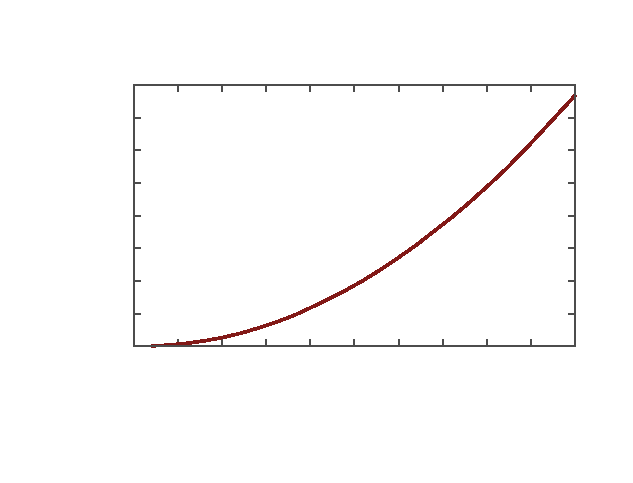
\includegraphics{./graficos/burbuja-linux-O0}}%
    \gplfronttext
  \end{picture}%
\endgroup

\end{center}

\subsubsection*{Insercción}
Consideramos el elemento N-ésimo de la lista y lo ordenamos respecto de los elementos desde el primero hasta el N-1-ésimo. Su eficiencia teórica es $O(n^2)$.
\begin{center}
	% GNUPLOT: LaTeX picture with Postscript
\begingroup
  \makeatletter
  \providecommand\color[2][]{%
    \GenericError{(gnuplot) \space\space\space\@spaces}{%
      Package color not loaded in conjunction with
      terminal option `colourtext'%
    }{See the gnuplot documentation for explanation.%
    }{Either use 'blacktext' in gnuplot or load the package
      color.sty in LaTeX.}%
    \renewcommand\color[2][]{}%
  }%
  \providecommand\includegraphics[2][]{%
    \GenericError{(gnuplot) \space\space\space\@spaces}{%
      Package graphicx or graphics not loaded%
    }{See the gnuplot documentation for explanation.%
    }{The gnuplot epslatex terminal needs graphicx.sty or graphics.sty.}%
    \renewcommand\includegraphics[2][]{}%
  }%
  \providecommand\rotatebox[2]{#2}%
  \@ifundefined{ifGPcolor}{%
    \newif\ifGPcolor
    \GPcolortrue
  }{}%
  \@ifundefined{ifGPblacktext}{%
    \newif\ifGPblacktext
    \GPblacktextfalse
  }{}%
  % define a \g@addto@macro without @ in the name:
  \let\gplgaddtomacro\g@addto@macro
  % define empty templates for all commands taking text:
  \gdef\gplbacktext{}%
  \gdef\gplfronttext{}%
  \makeatother
  \ifGPblacktext
    % no textcolor at all
    \def\colorrgb#1{}%
    \def\colorgray#1{}%
  \else
    % gray or color?
    \ifGPcolor
      \def\colorrgb#1{\color[rgb]{#1}}%
      \def\colorgray#1{\color[gray]{#1}}%
      \expandafter\def\csname LTw\endcsname{\color{white}}%
      \expandafter\def\csname LTb\endcsname{\color{black}}%
      \expandafter\def\csname LTa\endcsname{\color{black}}%
      \expandafter\def\csname LT0\endcsname{\color[rgb]{1,0,0}}%
      \expandafter\def\csname LT1\endcsname{\color[rgb]{0,1,0}}%
      \expandafter\def\csname LT2\endcsname{\color[rgb]{0,0,1}}%
      \expandafter\def\csname LT3\endcsname{\color[rgb]{1,0,1}}%
      \expandafter\def\csname LT4\endcsname{\color[rgb]{0,1,1}}%
      \expandafter\def\csname LT5\endcsname{\color[rgb]{1,1,0}}%
      \expandafter\def\csname LT6\endcsname{\color[rgb]{0,0,0}}%
      \expandafter\def\csname LT7\endcsname{\color[rgb]{1,0.3,0}}%
      \expandafter\def\csname LT8\endcsname{\color[rgb]{0.5,0.5,0.5}}%
    \else
      % gray
      \def\colorrgb#1{\color{black}}%
      \def\colorgray#1{\color[gray]{#1}}%
      \expandafter\def\csname LTw\endcsname{\color{white}}%
      \expandafter\def\csname LTb\endcsname{\color{black}}%
      \expandafter\def\csname LTa\endcsname{\color{black}}%
      \expandafter\def\csname LT0\endcsname{\color{black}}%
      \expandafter\def\csname LT1\endcsname{\color{black}}%
      \expandafter\def\csname LT2\endcsname{\color{black}}%
      \expandafter\def\csname LT3\endcsname{\color{black}}%
      \expandafter\def\csname LT4\endcsname{\color{black}}%
      \expandafter\def\csname LT5\endcsname{\color{black}}%
      \expandafter\def\csname LT6\endcsname{\color{black}}%
      \expandafter\def\csname LT7\endcsname{\color{black}}%
      \expandafter\def\csname LT8\endcsname{\color{black}}%
    \fi
  \fi
    \setlength{\unitlength}{0.0500bp}%
    \ifx\gptboxheight\undefined%
      \newlength{\gptboxheight}%
      \newlength{\gptboxwidth}%
      \newsavebox{\gptboxtext}%
    \fi%
    \setlength{\fboxrule}{0.5pt}%
    \setlength{\fboxsep}{1pt}%
\begin{picture}(5760.00,4320.00)%
    \gplgaddtomacro\gplbacktext{%
      \colorrgb{0.30,0.30,0.30}%
      \put(1254,1153){\makebox(0,0)[r]{\strut{}$\textcolor{text}{0}$}}%
      \colorrgb{0.30,0.30,0.30}%
      \put(1254,1571){\makebox(0,0)[r]{\strut{}$\textcolor{text}{0.5}$}}%
      \colorrgb{0.30,0.30,0.30}%
      \put(1254,1988){\makebox(0,0)[r]{\strut{}$\textcolor{text}{1}$}}%
      \colorrgb{0.30,0.30,0.30}%
      \put(1254,2406){\makebox(0,0)[r]{\strut{}$\textcolor{text}{1.5}$}}%
      \colorrgb{0.30,0.30,0.30}%
      \put(1254,2824){\makebox(0,0)[r]{\strut{}$\textcolor{text}{2}$}}%
      \colorrgb{0.30,0.30,0.30}%
      \put(1254,3241){\makebox(0,0)[r]{\strut{}$\textcolor{text}{2.5}$}}%
      \colorrgb{0.30,0.30,0.30}%
      \put(1254,3659){\makebox(0,0)[r]{\strut{}$\textcolor{text}{3}$}}%
      \colorrgb{0.30,0.30,0.30}%
      \put(1386,1021){\rotatebox{45}{\makebox(0,0)[r]{\strut{}$\textcolor{text}{0}$}}}%
      \colorrgb{0.30,0.30,0.30}%
      \put(1784,1021){\rotatebox{45}{\makebox(0,0)[r]{\strut{}$\textcolor{text}{5000}$}}}%
      \colorrgb{0.30,0.30,0.30}%
      \put(2181,1021){\rotatebox{45}{\makebox(0,0)[r]{\strut{}$\textcolor{text}{10000}$}}}%
      \colorrgb{0.30,0.30,0.30}%
      \put(2579,1021){\rotatebox{45}{\makebox(0,0)[r]{\strut{}$\textcolor{text}{15000}$}}}%
      \colorrgb{0.30,0.30,0.30}%
      \put(2977,1021){\rotatebox{45}{\makebox(0,0)[r]{\strut{}$\textcolor{text}{20000}$}}}%
      \colorrgb{0.30,0.30,0.30}%
      \put(3375,1021){\rotatebox{45}{\makebox(0,0)[r]{\strut{}$\textcolor{text}{25000}$}}}%
      \colorrgb{0.30,0.30,0.30}%
      \put(3772,1021){\rotatebox{45}{\makebox(0,0)[r]{\strut{}$\textcolor{text}{30000}$}}}%
      \colorrgb{0.30,0.30,0.30}%
      \put(4170,1021){\rotatebox{45}{\makebox(0,0)[r]{\strut{}$\textcolor{text}{35000}$}}}%
      \colorrgb{0.30,0.30,0.30}%
      \put(4568,1021){\rotatebox{45}{\makebox(0,0)[r]{\strut{}$\textcolor{text}{40000}$}}}%
      \colorrgb{0.30,0.30,0.30}%
      \put(4965,1021){\rotatebox{45}{\makebox(0,0)[r]{\strut{}$\textcolor{text}{45000}$}}}%
      \colorrgb{0.30,0.30,0.30}%
      \put(5363,1021){\rotatebox{45}{\makebox(0,0)[r]{\strut{}$\textcolor{text}{50000}$}}}%
    }%
    \gplgaddtomacro\gplfronttext{%
      \colorrgb{0.30,0.30,0.30}%
      \put(220,2406){\rotatebox{-270}{\makebox(0,0){\strut{}Tiempo de ejecución (s)}}}%
      \colorrgb{0.30,0.30,0.30}%
      \put(3374,220){\makebox(0,0){\strut{}Tamaño del vector (elementos)}}%
      \colorrgb{0.30,0.30,0.30}%
      \put(3374,3989){\makebox(0,0){\strut{}insercion-linux-O0}}%
    }%
    \gplbacktext
    \put(0,0){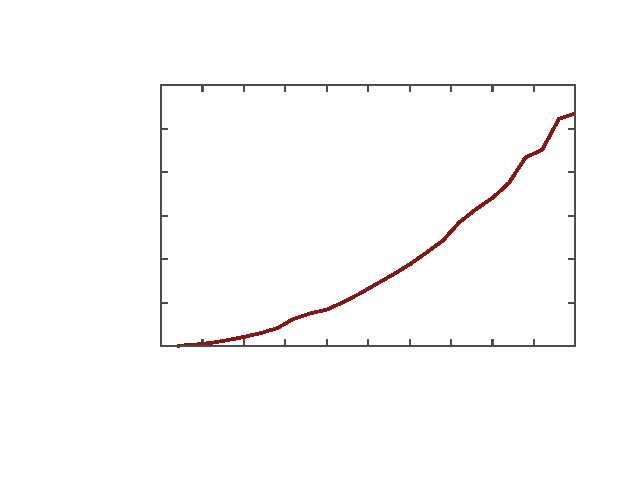
\includegraphics{./graficos/insercion-linux-O0}}%
    \gplfronttext
  \end{picture}%
\endgroup

\end{center}


\subsubsection*{Selección}
Consiste en encontrar el menor de todos los elementos de la lista e intercambiarlo con el de la primera posición. Luego con el segundo, y así sucesivamente hasta ordenarlo todo. De nuevo, su eficiencia teórica es $O(n^2)$.
\begin{center}
	% GNUPLOT: LaTeX picture with Postscript
\begingroup
  \makeatletter
  \providecommand\color[2][]{%
    \GenericError{(gnuplot) \space\space\space\@spaces}{%
      Package color not loaded in conjunction with
      terminal option `colourtext'%
    }{See the gnuplot documentation for explanation.%
    }{Either use 'blacktext' in gnuplot or load the package
      color.sty in LaTeX.}%
    \renewcommand\color[2][]{}%
  }%
  \providecommand\includegraphics[2][]{%
    \GenericError{(gnuplot) \space\space\space\@spaces}{%
      Package graphicx or graphics not loaded%
    }{See the gnuplot documentation for explanation.%
    }{The gnuplot epslatex terminal needs graphicx.sty or graphics.sty.}%
    \renewcommand\includegraphics[2][]{}%
  }%
  \providecommand\rotatebox[2]{#2}%
  \@ifundefined{ifGPcolor}{%
    \newif\ifGPcolor
    \GPcolortrue
  }{}%
  \@ifundefined{ifGPblacktext}{%
    \newif\ifGPblacktext
    \GPblacktextfalse
  }{}%
  % define a \g@addto@macro without @ in the name:
  \let\gplgaddtomacro\g@addto@macro
  % define empty templates for all commands taking text:
  \gdef\gplbacktext{}%
  \gdef\gplfronttext{}%
  \makeatother
  \ifGPblacktext
    % no textcolor at all
    \def\colorrgb#1{}%
    \def\colorgray#1{}%
  \else
    % gray or color?
    \ifGPcolor
      \def\colorrgb#1{\color[rgb]{#1}}%
      \def\colorgray#1{\color[gray]{#1}}%
      \expandafter\def\csname LTw\endcsname{\color{white}}%
      \expandafter\def\csname LTb\endcsname{\color{black}}%
      \expandafter\def\csname LTa\endcsname{\color{black}}%
      \expandafter\def\csname LT0\endcsname{\color[rgb]{1,0,0}}%
      \expandafter\def\csname LT1\endcsname{\color[rgb]{0,1,0}}%
      \expandafter\def\csname LT2\endcsname{\color[rgb]{0,0,1}}%
      \expandafter\def\csname LT3\endcsname{\color[rgb]{1,0,1}}%
      \expandafter\def\csname LT4\endcsname{\color[rgb]{0,1,1}}%
      \expandafter\def\csname LT5\endcsname{\color[rgb]{1,1,0}}%
      \expandafter\def\csname LT6\endcsname{\color[rgb]{0,0,0}}%
      \expandafter\def\csname LT7\endcsname{\color[rgb]{1,0.3,0}}%
      \expandafter\def\csname LT8\endcsname{\color[rgb]{0.5,0.5,0.5}}%
    \else
      % gray
      \def\colorrgb#1{\color{black}}%
      \def\colorgray#1{\color[gray]{#1}}%
      \expandafter\def\csname LTw\endcsname{\color{white}}%
      \expandafter\def\csname LTb\endcsname{\color{black}}%
      \expandafter\def\csname LTa\endcsname{\color{black}}%
      \expandafter\def\csname LT0\endcsname{\color{black}}%
      \expandafter\def\csname LT1\endcsname{\color{black}}%
      \expandafter\def\csname LT2\endcsname{\color{black}}%
      \expandafter\def\csname LT3\endcsname{\color{black}}%
      \expandafter\def\csname LT4\endcsname{\color{black}}%
      \expandafter\def\csname LT5\endcsname{\color{black}}%
      \expandafter\def\csname LT6\endcsname{\color{black}}%
      \expandafter\def\csname LT7\endcsname{\color{black}}%
      \expandafter\def\csname LT8\endcsname{\color{black}}%
    \fi
  \fi
    \setlength{\unitlength}{0.0500bp}%
    \ifx\gptboxheight\undefined%
      \newlength{\gptboxheight}%
      \newlength{\gptboxwidth}%
      \newsavebox{\gptboxtext}%
    \fi%
    \setlength{\fboxrule}{0.5pt}%
    \setlength{\fboxsep}{1pt}%
\begin{picture}(5760.00,4320.00)%
    \gplgaddtomacro\gplbacktext{%
      \colorrgb{0.30,0.30,0.30}%
      \put(1254,1153){\makebox(0,0)[r]{\strut{}$\textcolor{text}{0}$}}%
      \colorrgb{0.30,0.30,0.30}%
      \put(1254,1511){\makebox(0,0)[r]{\strut{}$\textcolor{text}{0.5}$}}%
      \colorrgb{0.30,0.30,0.30}%
      \put(1254,1869){\makebox(0,0)[r]{\strut{}$\textcolor{text}{1}$}}%
      \colorrgb{0.30,0.30,0.30}%
      \put(1254,2227){\makebox(0,0)[r]{\strut{}$\textcolor{text}{1.5}$}}%
      \colorrgb{0.30,0.30,0.30}%
      \put(1254,2585){\makebox(0,0)[r]{\strut{}$\textcolor{text}{2}$}}%
      \colorrgb{0.30,0.30,0.30}%
      \put(1254,2943){\makebox(0,0)[r]{\strut{}$\textcolor{text}{2.5}$}}%
      \colorrgb{0.30,0.30,0.30}%
      \put(1254,3301){\makebox(0,0)[r]{\strut{}$\textcolor{text}{3}$}}%
      \colorrgb{0.30,0.30,0.30}%
      \put(1254,3659){\makebox(0,0)[r]{\strut{}$\textcolor{text}{3.5}$}}%
      \colorrgb{0.30,0.30,0.30}%
      \put(1386,1021){\rotatebox{45}{\makebox(0,0)[r]{\strut{}$\textcolor{text}{0}$}}}%
      \colorrgb{0.30,0.30,0.30}%
      \put(1784,1021){\rotatebox{45}{\makebox(0,0)[r]{\strut{}$\textcolor{text}{5000}$}}}%
      \colorrgb{0.30,0.30,0.30}%
      \put(2181,1021){\rotatebox{45}{\makebox(0,0)[r]{\strut{}$\textcolor{text}{10000}$}}}%
      \colorrgb{0.30,0.30,0.30}%
      \put(2579,1021){\rotatebox{45}{\makebox(0,0)[r]{\strut{}$\textcolor{text}{15000}$}}}%
      \colorrgb{0.30,0.30,0.30}%
      \put(2977,1021){\rotatebox{45}{\makebox(0,0)[r]{\strut{}$\textcolor{text}{20000}$}}}%
      \colorrgb{0.30,0.30,0.30}%
      \put(3375,1021){\rotatebox{45}{\makebox(0,0)[r]{\strut{}$\textcolor{text}{25000}$}}}%
      \colorrgb{0.30,0.30,0.30}%
      \put(3772,1021){\rotatebox{45}{\makebox(0,0)[r]{\strut{}$\textcolor{text}{30000}$}}}%
      \colorrgb{0.30,0.30,0.30}%
      \put(4170,1021){\rotatebox{45}{\makebox(0,0)[r]{\strut{}$\textcolor{text}{35000}$}}}%
      \colorrgb{0.30,0.30,0.30}%
      \put(4568,1021){\rotatebox{45}{\makebox(0,0)[r]{\strut{}$\textcolor{text}{40000}$}}}%
      \colorrgb{0.30,0.30,0.30}%
      \put(4965,1021){\rotatebox{45}{\makebox(0,0)[r]{\strut{}$\textcolor{text}{45000}$}}}%
      \colorrgb{0.30,0.30,0.30}%
      \put(5363,1021){\rotatebox{45}{\makebox(0,0)[r]{\strut{}$\textcolor{text}{50000}$}}}%
    }%
    \gplgaddtomacro\gplfronttext{%
      \colorrgb{0.30,0.30,0.30}%
      \put(220,2406){\rotatebox{-270}{\makebox(0,0){\strut{}Tiempo de ejecución (s)}}}%
      \colorrgb{0.30,0.30,0.30}%
      \put(3374,220){\makebox(0,0){\strut{}Tamaño del vector (elementos)}}%
      \colorrgb{0.30,0.30,0.30}%
      \put(3374,3989){\makebox(0,0){\strut{}seleccion-linux-O0}}%
    }%
    \gplbacktext
    \put(0,0){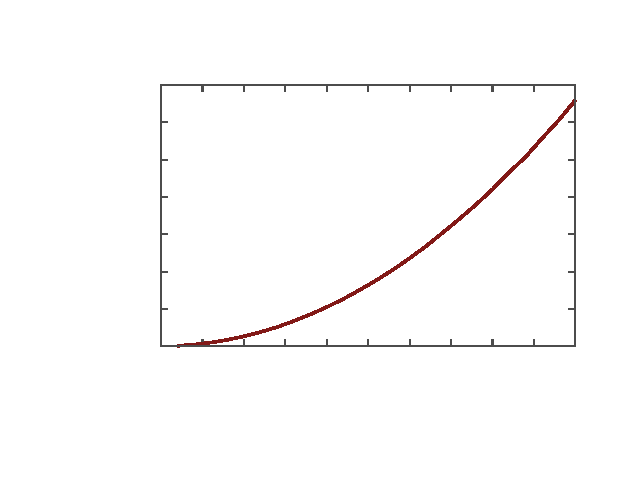
\includegraphics{./graficos/seleccion-linux-O0}}%
    \gplfronttext
  \end{picture}%
\endgroup

\end{center}

\subsection*{Eficiencia $\boldsymbol{n log n}$}
\subsubsection*{Mergesort}
Se basa en la técnica de divide y vencerás. Consiste en dividir la lista en sublistas de la mitad de tamaño, ordenando cada una de ellas de forma recursiva. Si el tamaño de la lista es 0 ó 1 la lista ya está ordenada. Para acabar juntamos todas las sublistas en una sola. Su eficiencia teórica es $O(n\log n)$.

\begin{center}
	% GNUPLOT: LaTeX picture with Postscript
\begingroup
  \makeatletter
  \providecommand\color[2][]{%
    \GenericError{(gnuplot) \space\space\space\@spaces}{%
      Package color not loaded in conjunction with
      terminal option `colourtext'%
    }{See the gnuplot documentation for explanation.%
    }{Either use 'blacktext' in gnuplot or load the package
      color.sty in LaTeX.}%
    \renewcommand\color[2][]{}%
  }%
  \providecommand\includegraphics[2][]{%
    \GenericError{(gnuplot) \space\space\space\@spaces}{%
      Package graphicx or graphics not loaded%
    }{See the gnuplot documentation for explanation.%
    }{The gnuplot epslatex terminal needs graphicx.sty or graphics.sty.}%
    \renewcommand\includegraphics[2][]{}%
  }%
  \providecommand\rotatebox[2]{#2}%
  \@ifundefined{ifGPcolor}{%
    \newif\ifGPcolor
    \GPcolortrue
  }{}%
  \@ifundefined{ifGPblacktext}{%
    \newif\ifGPblacktext
    \GPblacktextfalse
  }{}%
  % define a \g@addto@macro without @ in the name:
  \let\gplgaddtomacro\g@addto@macro
  % define empty templates for all commands taking text:
  \gdef\gplbacktext{}%
  \gdef\gplfronttext{}%
  \makeatother
  \ifGPblacktext
    % no textcolor at all
    \def\colorrgb#1{}%
    \def\colorgray#1{}%
  \else
    % gray or color?
    \ifGPcolor
      \def\colorrgb#1{\color[rgb]{#1}}%
      \def\colorgray#1{\color[gray]{#1}}%
      \expandafter\def\csname LTw\endcsname{\color{white}}%
      \expandafter\def\csname LTb\endcsname{\color{black}}%
      \expandafter\def\csname LTa\endcsname{\color{black}}%
      \expandafter\def\csname LT0\endcsname{\color[rgb]{1,0,0}}%
      \expandafter\def\csname LT1\endcsname{\color[rgb]{0,1,0}}%
      \expandafter\def\csname LT2\endcsname{\color[rgb]{0,0,1}}%
      \expandafter\def\csname LT3\endcsname{\color[rgb]{1,0,1}}%
      \expandafter\def\csname LT4\endcsname{\color[rgb]{0,1,1}}%
      \expandafter\def\csname LT5\endcsname{\color[rgb]{1,1,0}}%
      \expandafter\def\csname LT6\endcsname{\color[rgb]{0,0,0}}%
      \expandafter\def\csname LT7\endcsname{\color[rgb]{1,0.3,0}}%
      \expandafter\def\csname LT8\endcsname{\color[rgb]{0.5,0.5,0.5}}%
    \else
      % gray
      \def\colorrgb#1{\color{black}}%
      \def\colorgray#1{\color[gray]{#1}}%
      \expandafter\def\csname LTw\endcsname{\color{white}}%
      \expandafter\def\csname LTb\endcsname{\color{black}}%
      \expandafter\def\csname LTa\endcsname{\color{black}}%
      \expandafter\def\csname LT0\endcsname{\color{black}}%
      \expandafter\def\csname LT1\endcsname{\color{black}}%
      \expandafter\def\csname LT2\endcsname{\color{black}}%
      \expandafter\def\csname LT3\endcsname{\color{black}}%
      \expandafter\def\csname LT4\endcsname{\color{black}}%
      \expandafter\def\csname LT5\endcsname{\color{black}}%
      \expandafter\def\csname LT6\endcsname{\color{black}}%
      \expandafter\def\csname LT7\endcsname{\color{black}}%
      \expandafter\def\csname LT8\endcsname{\color{black}}%
    \fi
  \fi
    \setlength{\unitlength}{0.0500bp}%
    \ifx\gptboxheight\undefined%
      \newlength{\gptboxheight}%
      \newlength{\gptboxwidth}%
      \newsavebox{\gptboxtext}%
    \fi%
    \setlength{\fboxrule}{0.5pt}%
    \setlength{\fboxsep}{1pt}%
\begin{picture}(5760.00,4320.00)%
    \gplgaddtomacro\gplbacktext{%
      \colorrgb{0.30,0.30,0.30}%
      \put(1518,1246){\makebox(0,0)[r]{\strut{}$\textcolor{text}{0}$}}%
      \colorrgb{0.30,0.30,0.30}%
      \put(1518,1591){\makebox(0,0)[r]{\strut{}$\textcolor{text}{0.005}$}}%
      \colorrgb{0.30,0.30,0.30}%
      \put(1518,1935){\makebox(0,0)[r]{\strut{}$\textcolor{text}{0.01}$}}%
      \colorrgb{0.30,0.30,0.30}%
      \put(1518,2280){\makebox(0,0)[r]{\strut{}$\textcolor{text}{0.015}$}}%
      \colorrgb{0.30,0.30,0.30}%
      \put(1518,2625){\makebox(0,0)[r]{\strut{}$\textcolor{text}{0.02}$}}%
      \colorrgb{0.30,0.30,0.30}%
      \put(1518,2970){\makebox(0,0)[r]{\strut{}$\textcolor{text}{0.025}$}}%
      \colorrgb{0.30,0.30,0.30}%
      \put(1518,3314){\makebox(0,0)[r]{\strut{}$\textcolor{text}{0.03}$}}%
      \colorrgb{0.30,0.30,0.30}%
      \put(1518,3659){\makebox(0,0)[r]{\strut{}$\textcolor{text}{0.035}$}}%
      \colorrgb{0.30,0.30,0.30}%
      \put(1650,1114){\rotatebox{45}{\makebox(0,0)[r]{\strut{}$\textcolor{text}{0}$}}}%
      \colorrgb{0.30,0.30,0.30}%
      \put(2114,1114){\rotatebox{45}{\makebox(0,0)[r]{\strut{}$\textcolor{text}{20000}$}}}%
      \colorrgb{0.30,0.30,0.30}%
      \put(2578,1114){\rotatebox{45}{\makebox(0,0)[r]{\strut{}$\textcolor{text}{40000}$}}}%
      \colorrgb{0.30,0.30,0.30}%
      \put(3042,1114){\rotatebox{45}{\makebox(0,0)[r]{\strut{}$\textcolor{text}{60000}$}}}%
      \colorrgb{0.30,0.30,0.30}%
      \put(3507,1114){\rotatebox{45}{\makebox(0,0)[r]{\strut{}$\textcolor{text}{80000}$}}}%
      \colorrgb{0.30,0.30,0.30}%
      \put(3971,1114){\rotatebox{45}{\makebox(0,0)[r]{\strut{}$\textcolor{text}{100000}$}}}%
      \colorrgb{0.30,0.30,0.30}%
      \put(4435,1114){\rotatebox{45}{\makebox(0,0)[r]{\strut{}$\textcolor{text}{120000}$}}}%
      \colorrgb{0.30,0.30,0.30}%
      \put(4899,1114){\rotatebox{45}{\makebox(0,0)[r]{\strut{}$\textcolor{text}{140000}$}}}%
      \colorrgb{0.30,0.30,0.30}%
      \put(5363,1114){\rotatebox{45}{\makebox(0,0)[r]{\strut{}$\textcolor{text}{160000}$}}}%
    }%
    \gplgaddtomacro\gplfronttext{%
      \colorrgb{0.30,0.30,0.30}%
      \put(220,2452){\rotatebox{-270}{\makebox(0,0){\strut{}Tiempo de ejecución (s)}}}%
      \colorrgb{0.30,0.30,0.30}%
      \put(3506,220){\makebox(0,0){\strut{}Tamaño del vector (elementos)}}%
      \colorrgb{0.30,0.30,0.30}%
      \put(3506,3989){\makebox(0,0){\strut{}mergesort-linux-O0}}%
    }%
    \gplbacktext
    \put(0,0){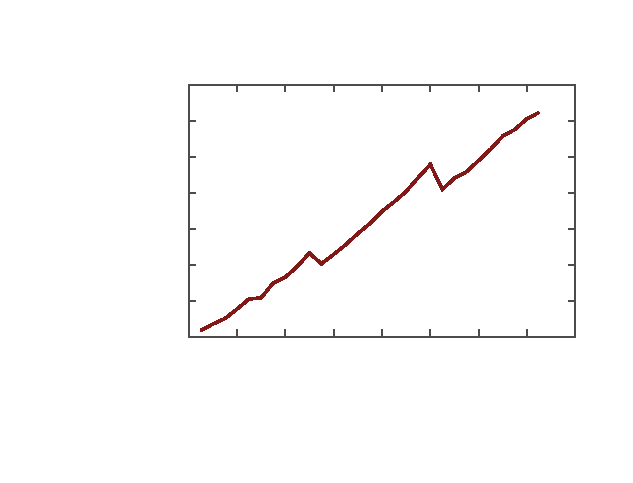
\includegraphics{./graficos/mergesort-linux-O0}}%
    \gplfronttext
  \end{picture}%
\endgroup

\end{center}

Podemos observar algunos picos en la gráfica pero no sabemos a que puede ser debido.

\subsubsection*{Quicksort}
También se basa en la técnica de divide y vencerás.
En primer lugar elegimos un elemento de la lista, que llamaremos \textit{pivote}. A continuación los elementos de la lista se ordenarán de forma que la derecha del pivote queden los mayores y a la izquierda los menores. De esta forma dividimos la lista en dos sublistas, la de la derecha y la de la izquierda. Repetiremos el proceso mientras las sublistas tengan más de un elemento. Su eficiencia teórica también es $O(n\log n)$.

\begin{center}
	% GNUPLOT: LaTeX picture with Postscript
\begingroup
  \makeatletter
  \providecommand\color[2][]{%
    \GenericError{(gnuplot) \space\space\space\@spaces}{%
      Package color not loaded in conjunction with
      terminal option `colourtext'%
    }{See the gnuplot documentation for explanation.%
    }{Either use 'blacktext' in gnuplot or load the package
      color.sty in LaTeX.}%
    \renewcommand\color[2][]{}%
  }%
  \providecommand\includegraphics[2][]{%
    \GenericError{(gnuplot) \space\space\space\@spaces}{%
      Package graphicx or graphics not loaded%
    }{See the gnuplot documentation for explanation.%
    }{The gnuplot epslatex terminal needs graphicx.sty or graphics.sty.}%
    \renewcommand\includegraphics[2][]{}%
  }%
  \providecommand\rotatebox[2]{#2}%
  \@ifundefined{ifGPcolor}{%
    \newif\ifGPcolor
    \GPcolortrue
  }{}%
  \@ifundefined{ifGPblacktext}{%
    \newif\ifGPblacktext
    \GPblacktextfalse
  }{}%
  % define a \g@addto@macro without @ in the name:
  \let\gplgaddtomacro\g@addto@macro
  % define empty templates for all commands taking text:
  \gdef\gplbacktext{}%
  \gdef\gplfronttext{}%
  \makeatother
  \ifGPblacktext
    % no textcolor at all
    \def\colorrgb#1{}%
    \def\colorgray#1{}%
  \else
    % gray or color?
    \ifGPcolor
      \def\colorrgb#1{\color[rgb]{#1}}%
      \def\colorgray#1{\color[gray]{#1}}%
      \expandafter\def\csname LTw\endcsname{\color{white}}%
      \expandafter\def\csname LTb\endcsname{\color{black}}%
      \expandafter\def\csname LTa\endcsname{\color{black}}%
      \expandafter\def\csname LT0\endcsname{\color[rgb]{1,0,0}}%
      \expandafter\def\csname LT1\endcsname{\color[rgb]{0,1,0}}%
      \expandafter\def\csname LT2\endcsname{\color[rgb]{0,0,1}}%
      \expandafter\def\csname LT3\endcsname{\color[rgb]{1,0,1}}%
      \expandafter\def\csname LT4\endcsname{\color[rgb]{0,1,1}}%
      \expandafter\def\csname LT5\endcsname{\color[rgb]{1,1,0}}%
      \expandafter\def\csname LT6\endcsname{\color[rgb]{0,0,0}}%
      \expandafter\def\csname LT7\endcsname{\color[rgb]{1,0.3,0}}%
      \expandafter\def\csname LT8\endcsname{\color[rgb]{0.5,0.5,0.5}}%
    \else
      % gray
      \def\colorrgb#1{\color{black}}%
      \def\colorgray#1{\color[gray]{#1}}%
      \expandafter\def\csname LTw\endcsname{\color{white}}%
      \expandafter\def\csname LTb\endcsname{\color{black}}%
      \expandafter\def\csname LTa\endcsname{\color{black}}%
      \expandafter\def\csname LT0\endcsname{\color{black}}%
      \expandafter\def\csname LT1\endcsname{\color{black}}%
      \expandafter\def\csname LT2\endcsname{\color{black}}%
      \expandafter\def\csname LT3\endcsname{\color{black}}%
      \expandafter\def\csname LT4\endcsname{\color{black}}%
      \expandafter\def\csname LT5\endcsname{\color{black}}%
      \expandafter\def\csname LT6\endcsname{\color{black}}%
      \expandafter\def\csname LT7\endcsname{\color{black}}%
      \expandafter\def\csname LT8\endcsname{\color{black}}%
    \fi
  \fi
    \setlength{\unitlength}{0.0500bp}%
    \ifx\gptboxheight\undefined%
      \newlength{\gptboxheight}%
      \newlength{\gptboxwidth}%
      \newsavebox{\gptboxtext}%
    \fi%
    \setlength{\fboxrule}{0.5pt}%
    \setlength{\fboxsep}{1pt}%
\begin{picture}(5760.00,4320.00)%
    \gplgaddtomacro\gplbacktext{%
      \colorrgb{0.30,0.30,0.30}%
      \put(1650,1246){\makebox(0,0)[r]{\strut{}$\textcolor{text}{0.0001}$}}%
      \colorrgb{0.30,0.30,0.30}%
      \put(1650,2050){\makebox(0,0)[r]{\strut{}$\textcolor{text}{0.001}$}}%
      \colorrgb{0.30,0.30,0.30}%
      \put(1650,2855){\makebox(0,0)[r]{\strut{}$\textcolor{text}{0.01}$}}%
      \colorrgb{0.30,0.30,0.30}%
      \put(1650,3659){\makebox(0,0)[r]{\strut{}$\textcolor{text}{0.1}$}}%
      \colorrgb{0.30,0.30,0.30}%
      \put(1782,1114){\rotatebox{45}{\makebox(0,0)[r]{\strut{}$\textcolor{text}{0}$}}}%
      \colorrgb{0.30,0.30,0.30}%
      \put(2230,1114){\rotatebox{45}{\makebox(0,0)[r]{\strut{}$\textcolor{text}{20000}$}}}%
      \colorrgb{0.30,0.30,0.30}%
      \put(2677,1114){\rotatebox{45}{\makebox(0,0)[r]{\strut{}$\textcolor{text}{40000}$}}}%
      \colorrgb{0.30,0.30,0.30}%
      \put(3125,1114){\rotatebox{45}{\makebox(0,0)[r]{\strut{}$\textcolor{text}{60000}$}}}%
      \colorrgb{0.30,0.30,0.30}%
      \put(3573,1114){\rotatebox{45}{\makebox(0,0)[r]{\strut{}$\textcolor{text}{80000}$}}}%
      \colorrgb{0.30,0.30,0.30}%
      \put(4020,1114){\rotatebox{45}{\makebox(0,0)[r]{\strut{}$\textcolor{text}{100000}$}}}%
      \colorrgb{0.30,0.30,0.30}%
      \put(4468,1114){\rotatebox{45}{\makebox(0,0)[r]{\strut{}$\textcolor{text}{120000}$}}}%
      \colorrgb{0.30,0.30,0.30}%
      \put(4915,1114){\rotatebox{45}{\makebox(0,0)[r]{\strut{}$\textcolor{text}{140000}$}}}%
      \colorrgb{0.30,0.30,0.30}%
      \put(5363,1114){\rotatebox{45}{\makebox(0,0)[r]{\strut{}$\textcolor{text}{160000}$}}}%
    }%
    \gplgaddtomacro\gplfronttext{%
      \colorrgb{0.30,0.30,0.30}%
      \put(220,2452){\rotatebox{-270}{\makebox(0,0){\strut{}Tiempo de ejecución (s)}}}%
      \colorrgb{0.30,0.30,0.30}%
      \put(3572,220){\makebox(0,0){\strut{}Tamaño del vector (elementos)}}%
      \colorrgb{0.30,0.30,0.30}%
      \put(3572,3989){\makebox(0,0){\strut{}quicksort-linux-O0}}%
    }%
    \gplbacktext
    \put(0,0){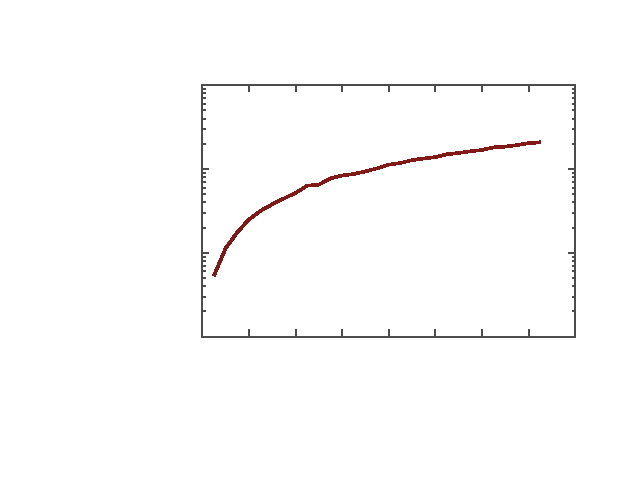
\includegraphics{./graficos/quicksort-linux-O0}}%
    \gplfronttext
  \end{picture}%
\endgroup

\end{center}

\subsubsection*{Heapsort}
Este algoritmo consiste en almacenar todos los elementos del vector a ordenar en una estructura de datos llamada montículo (\textit{heap}). Luego, se extrae el nodo que queda como nodo raíz del montículo (cima) en sucesivas iteraciones obteniendo el conjunto ordenado. Basa su funcionamiento en una propiedad de los montículos, por la cual, la cima contiene siempre el menor elemento (o el mayor, según se haya definido el montículo) de todos los almacenados en él. Su eficiencia teórica es $O(n\log n)$.
\begin{center}
	% GNUPLOT: LaTeX picture with Postscript
\begingroup
  \makeatletter
  \providecommand\color[2][]{%
    \GenericError{(gnuplot) \space\space\space\@spaces}{%
      Package color not loaded in conjunction with
      terminal option `colourtext'%
    }{See the gnuplot documentation for explanation.%
    }{Either use 'blacktext' in gnuplot or load the package
      color.sty in LaTeX.}%
    \renewcommand\color[2][]{}%
  }%
  \providecommand\includegraphics[2][]{%
    \GenericError{(gnuplot) \space\space\space\@spaces}{%
      Package graphicx or graphics not loaded%
    }{See the gnuplot documentation for explanation.%
    }{The gnuplot epslatex terminal needs graphicx.sty or graphics.sty.}%
    \renewcommand\includegraphics[2][]{}%
  }%
  \providecommand\rotatebox[2]{#2}%
  \@ifundefined{ifGPcolor}{%
    \newif\ifGPcolor
    \GPcolortrue
  }{}%
  \@ifundefined{ifGPblacktext}{%
    \newif\ifGPblacktext
    \GPblacktextfalse
  }{}%
  % define a \g@addto@macro without @ in the name:
  \let\gplgaddtomacro\g@addto@macro
  % define empty templates for all commands taking text:
  \gdef\gplbacktext{}%
  \gdef\gplfronttext{}%
  \makeatother
  \ifGPblacktext
    % no textcolor at all
    \def\colorrgb#1{}%
    \def\colorgray#1{}%
  \else
    % gray or color?
    \ifGPcolor
      \def\colorrgb#1{\color[rgb]{#1}}%
      \def\colorgray#1{\color[gray]{#1}}%
      \expandafter\def\csname LTw\endcsname{\color{white}}%
      \expandafter\def\csname LTb\endcsname{\color{black}}%
      \expandafter\def\csname LTa\endcsname{\color{black}}%
      \expandafter\def\csname LT0\endcsname{\color[rgb]{1,0,0}}%
      \expandafter\def\csname LT1\endcsname{\color[rgb]{0,1,0}}%
      \expandafter\def\csname LT2\endcsname{\color[rgb]{0,0,1}}%
      \expandafter\def\csname LT3\endcsname{\color[rgb]{1,0,1}}%
      \expandafter\def\csname LT4\endcsname{\color[rgb]{0,1,1}}%
      \expandafter\def\csname LT5\endcsname{\color[rgb]{1,1,0}}%
      \expandafter\def\csname LT6\endcsname{\color[rgb]{0,0,0}}%
      \expandafter\def\csname LT7\endcsname{\color[rgb]{1,0.3,0}}%
      \expandafter\def\csname LT8\endcsname{\color[rgb]{0.5,0.5,0.5}}%
    \else
      % gray
      \def\colorrgb#1{\color{black}}%
      \def\colorgray#1{\color[gray]{#1}}%
      \expandafter\def\csname LTw\endcsname{\color{white}}%
      \expandafter\def\csname LTb\endcsname{\color{black}}%
      \expandafter\def\csname LTa\endcsname{\color{black}}%
      \expandafter\def\csname LT0\endcsname{\color{black}}%
      \expandafter\def\csname LT1\endcsname{\color{black}}%
      \expandafter\def\csname LT2\endcsname{\color{black}}%
      \expandafter\def\csname LT3\endcsname{\color{black}}%
      \expandafter\def\csname LT4\endcsname{\color{black}}%
      \expandafter\def\csname LT5\endcsname{\color{black}}%
      \expandafter\def\csname LT6\endcsname{\color{black}}%
      \expandafter\def\csname LT7\endcsname{\color{black}}%
      \expandafter\def\csname LT8\endcsname{\color{black}}%
    \fi
  \fi
    \setlength{\unitlength}{0.0500bp}%
    \ifx\gptboxheight\undefined%
      \newlength{\gptboxheight}%
      \newlength{\gptboxwidth}%
      \newsavebox{\gptboxtext}%
    \fi%
    \setlength{\fboxrule}{0.5pt}%
    \setlength{\fboxsep}{1pt}%
\begin{picture}(5760.00,4320.00)%
    \gplgaddtomacro\gplbacktext{%
      \colorrgb{0.30,0.30,0.30}%
      \put(1650,1246){\makebox(0,0)[r]{\strut{}$\textcolor{text}{0.0001}$}}%
      \colorrgb{0.30,0.30,0.30}%
      \put(1650,2050){\makebox(0,0)[r]{\strut{}$\textcolor{text}{0.001}$}}%
      \colorrgb{0.30,0.30,0.30}%
      \put(1650,2855){\makebox(0,0)[r]{\strut{}$\textcolor{text}{0.01}$}}%
      \colorrgb{0.30,0.30,0.30}%
      \put(1650,3659){\makebox(0,0)[r]{\strut{}$\textcolor{text}{0.1}$}}%
      \colorrgb{0.30,0.30,0.30}%
      \put(1782,1114){\rotatebox{45}{\makebox(0,0)[r]{\strut{}$\textcolor{text}{0}$}}}%
      \colorrgb{0.30,0.30,0.30}%
      \put(2230,1114){\rotatebox{45}{\makebox(0,0)[r]{\strut{}$\textcolor{text}{20000}$}}}%
      \colorrgb{0.30,0.30,0.30}%
      \put(2677,1114){\rotatebox{45}{\makebox(0,0)[r]{\strut{}$\textcolor{text}{40000}$}}}%
      \colorrgb{0.30,0.30,0.30}%
      \put(3125,1114){\rotatebox{45}{\makebox(0,0)[r]{\strut{}$\textcolor{text}{60000}$}}}%
      \colorrgb{0.30,0.30,0.30}%
      \put(3573,1114){\rotatebox{45}{\makebox(0,0)[r]{\strut{}$\textcolor{text}{80000}$}}}%
      \colorrgb{0.30,0.30,0.30}%
      \put(4020,1114){\rotatebox{45}{\makebox(0,0)[r]{\strut{}$\textcolor{text}{100000}$}}}%
      \colorrgb{0.30,0.30,0.30}%
      \put(4468,1114){\rotatebox{45}{\makebox(0,0)[r]{\strut{}$\textcolor{text}{120000}$}}}%
      \colorrgb{0.30,0.30,0.30}%
      \put(4915,1114){\rotatebox{45}{\makebox(0,0)[r]{\strut{}$\textcolor{text}{140000}$}}}%
      \colorrgb{0.30,0.30,0.30}%
      \put(5363,1114){\rotatebox{45}{\makebox(0,0)[r]{\strut{}$\textcolor{text}{160000}$}}}%
    }%
    \gplgaddtomacro\gplfronttext{%
      \colorrgb{0.30,0.30,0.30}%
      \put(220,2452){\rotatebox{-270}{\makebox(0,0){\strut{}Tiempo de ejecución (s)}}}%
      \colorrgb{0.30,0.30,0.30}%
      \put(3572,220){\makebox(0,0){\strut{}Tamaño del vector (elementos)}}%
      \colorrgb{0.30,0.30,0.30}%
      \put(3572,3989){\makebox(0,0){\strut{}heapsort-linux-O0}}%
    }%
    \gplbacktext
    \put(0,0){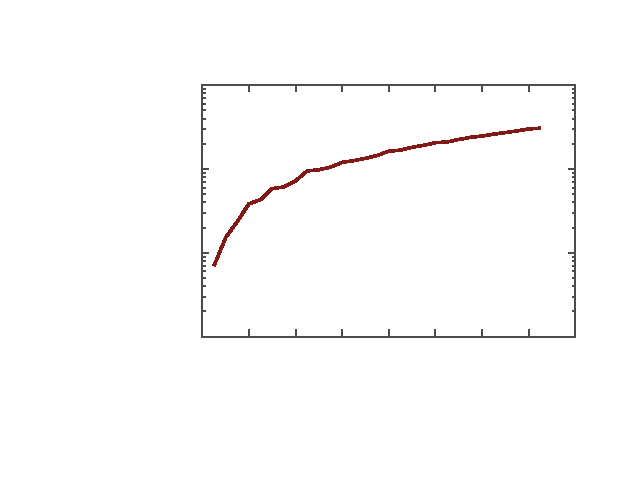
\includegraphics{./graficos/heapsort-linux-O0}}%
    \gplfronttext
  \end{picture}%
\endgroup

\end{center}

\section*{Otros algoritmos}

\subsection*{Floyd}
Es un algoritmo de análisis sobre grados para encontrar el camino mínimo en grafos ponderados. El algoritmo compara todos los posibles caminos a través del grafo entre cada par de vértices. Es un ejemplo de \textbf{programación dinámica}, y su eficiencia teórica es $O(n^3)$.

\begin{center}
	% GNUPLOT: LaTeX picture with Postscript
\begingroup
  \makeatletter
  \providecommand\color[2][]{%
    \GenericError{(gnuplot) \space\space\space\@spaces}{%
      Package color not loaded in conjunction with
      terminal option `colourtext'%
    }{See the gnuplot documentation for explanation.%
    }{Either use 'blacktext' in gnuplot or load the package
      color.sty in LaTeX.}%
    \renewcommand\color[2][]{}%
  }%
  \providecommand\includegraphics[2][]{%
    \GenericError{(gnuplot) \space\space\space\@spaces}{%
      Package graphicx or graphics not loaded%
    }{See the gnuplot documentation for explanation.%
    }{The gnuplot epslatex terminal needs graphicx.sty or graphics.sty.}%
    \renewcommand\includegraphics[2][]{}%
  }%
  \providecommand\rotatebox[2]{#2}%
  \@ifundefined{ifGPcolor}{%
    \newif\ifGPcolor
    \GPcolortrue
  }{}%
  \@ifundefined{ifGPblacktext}{%
    \newif\ifGPblacktext
    \GPblacktextfalse
  }{}%
  % define a \g@addto@macro without @ in the name:
  \let\gplgaddtomacro\g@addto@macro
  % define empty templates for all commands taking text:
  \gdef\gplbacktext{}%
  \gdef\gplfronttext{}%
  \makeatother
  \ifGPblacktext
    % no textcolor at all
    \def\colorrgb#1{}%
    \def\colorgray#1{}%
  \else
    % gray or color?
    \ifGPcolor
      \def\colorrgb#1{\color[rgb]{#1}}%
      \def\colorgray#1{\color[gray]{#1}}%
      \expandafter\def\csname LTw\endcsname{\color{white}}%
      \expandafter\def\csname LTb\endcsname{\color{black}}%
      \expandafter\def\csname LTa\endcsname{\color{black}}%
      \expandafter\def\csname LT0\endcsname{\color[rgb]{1,0,0}}%
      \expandafter\def\csname LT1\endcsname{\color[rgb]{0,1,0}}%
      \expandafter\def\csname LT2\endcsname{\color[rgb]{0,0,1}}%
      \expandafter\def\csname LT3\endcsname{\color[rgb]{1,0,1}}%
      \expandafter\def\csname LT4\endcsname{\color[rgb]{0,1,1}}%
      \expandafter\def\csname LT5\endcsname{\color[rgb]{1,1,0}}%
      \expandafter\def\csname LT6\endcsname{\color[rgb]{0,0,0}}%
      \expandafter\def\csname LT7\endcsname{\color[rgb]{1,0.3,0}}%
      \expandafter\def\csname LT8\endcsname{\color[rgb]{0.5,0.5,0.5}}%
    \else
      % gray
      \def\colorrgb#1{\color{black}}%
      \def\colorgray#1{\color[gray]{#1}}%
      \expandafter\def\csname LTw\endcsname{\color{white}}%
      \expandafter\def\csname LTb\endcsname{\color{black}}%
      \expandafter\def\csname LTa\endcsname{\color{black}}%
      \expandafter\def\csname LT0\endcsname{\color{black}}%
      \expandafter\def\csname LT1\endcsname{\color{black}}%
      \expandafter\def\csname LT2\endcsname{\color{black}}%
      \expandafter\def\csname LT3\endcsname{\color{black}}%
      \expandafter\def\csname LT4\endcsname{\color{black}}%
      \expandafter\def\csname LT5\endcsname{\color{black}}%
      \expandafter\def\csname LT6\endcsname{\color{black}}%
      \expandafter\def\csname LT7\endcsname{\color{black}}%
      \expandafter\def\csname LT8\endcsname{\color{black}}%
    \fi
  \fi
    \setlength{\unitlength}{0.0500bp}%
    \ifx\gptboxheight\undefined%
      \newlength{\gptboxheight}%
      \newlength{\gptboxwidth}%
      \newsavebox{\gptboxtext}%
    \fi%
    \setlength{\fboxrule}{0.5pt}%
    \setlength{\fboxsep}{1pt}%
\begin{picture}(5760.00,4320.00)%
    \gplgaddtomacro\gplbacktext{%
      \colorrgb{0.30,0.30,0.30}%
      \put(1122,1060){\makebox(0,0)[r]{\strut{}$\textcolor{text}{0}$}}%
      \colorrgb{0.30,0.30,0.30}%
      \put(1122,1349){\makebox(0,0)[r]{\strut{}$\textcolor{text}{2}$}}%
      \colorrgb{0.30,0.30,0.30}%
      \put(1122,1638){\makebox(0,0)[r]{\strut{}$\textcolor{text}{4}$}}%
      \colorrgb{0.30,0.30,0.30}%
      \put(1122,1926){\makebox(0,0)[r]{\strut{}$\textcolor{text}{6}$}}%
      \colorrgb{0.30,0.30,0.30}%
      \put(1122,2215){\makebox(0,0)[r]{\strut{}$\textcolor{text}{8}$}}%
      \colorrgb{0.30,0.30,0.30}%
      \put(1122,2504){\makebox(0,0)[r]{\strut{}$\textcolor{text}{10}$}}%
      \colorrgb{0.30,0.30,0.30}%
      \put(1122,2793){\makebox(0,0)[r]{\strut{}$\textcolor{text}{12}$}}%
      \colorrgb{0.30,0.30,0.30}%
      \put(1122,3081){\makebox(0,0)[r]{\strut{}$\textcolor{text}{14}$}}%
      \colorrgb{0.30,0.30,0.30}%
      \put(1122,3370){\makebox(0,0)[r]{\strut{}$\textcolor{text}{16}$}}%
      \colorrgb{0.30,0.30,0.30}%
      \put(1122,3659){\makebox(0,0)[r]{\strut{}$\textcolor{text}{18}$}}%
      \colorrgb{0.30,0.30,0.30}%
      \put(1254,928){\rotatebox{45}{\makebox(0,0)[r]{\strut{}$\textcolor{text}{0}$}}}%
      \colorrgb{0.30,0.30,0.30}%
      \put(1768,928){\rotatebox{45}{\makebox(0,0)[r]{\strut{}$\textcolor{text}{200}$}}}%
      \colorrgb{0.30,0.30,0.30}%
      \put(2281,928){\rotatebox{45}{\makebox(0,0)[r]{\strut{}$\textcolor{text}{400}$}}}%
      \colorrgb{0.30,0.30,0.30}%
      \put(2795,928){\rotatebox{45}{\makebox(0,0)[r]{\strut{}$\textcolor{text}{600}$}}}%
      \colorrgb{0.30,0.30,0.30}%
      \put(3309,928){\rotatebox{45}{\makebox(0,0)[r]{\strut{}$\textcolor{text}{800}$}}}%
      \colorrgb{0.30,0.30,0.30}%
      \put(3822,928){\rotatebox{45}{\makebox(0,0)[r]{\strut{}$\textcolor{text}{1000}$}}}%
      \colorrgb{0.30,0.30,0.30}%
      \put(4336,928){\rotatebox{45}{\makebox(0,0)[r]{\strut{}$\textcolor{text}{1200}$}}}%
      \colorrgb{0.30,0.30,0.30}%
      \put(4849,928){\rotatebox{45}{\makebox(0,0)[r]{\strut{}$\textcolor{text}{1400}$}}}%
      \colorrgb{0.30,0.30,0.30}%
      \put(5363,928){\rotatebox{45}{\makebox(0,0)[r]{\strut{}$\textcolor{text}{1600}$}}}%
    }%
    \gplgaddtomacro\gplfronttext{%
      \colorrgb{0.30,0.30,0.30}%
      \put(220,2359){\rotatebox{-270}{\makebox(0,0){\strut{}Tiempo de ejecución (s)}}}%
      \colorrgb{0.30,0.30,0.30}%
      \put(3308,220){\makebox(0,0){\strut{}Tamaño del grafo (vértices)}}%
      \colorrgb{0.30,0.30,0.30}%
      \put(3308,3989){\makebox(0,0){\strut{}Eficiencia empírica floyd-linux-O0}}%
    }%
    \gplbacktext
    \put(0,0){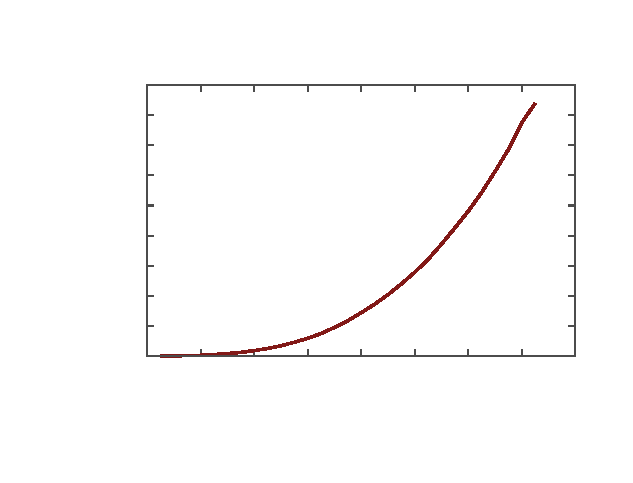
\includegraphics{./graficos/floyd-linux-O0}}%
    \gplfronttext
  \end{picture}%
\endgroup

\end{center}

\subsection*{Hanoi}
Hay tres pilas de discos, llamadas origen, auxiliar y destino. La primera de ellas está ordenada según tamaño creciente de los discos, de arriba hacia abajo. Se moverá un disco de la pila origen a la destino si hay un único disco en la pila origen. En caso contrario, se moverán todos los discos a la auxiliar, excepto el más grande. Por último, moveremos el disco mayor al destino, y movemos los $n-1$ restantes encima del mayor. El número de pasos crece exponencialmente con el número de discos, y su eficiencia teórica es $O(2^n)$.

\begin{center}
	% GNUPLOT: LaTeX picture with Postscript
\begingroup
  \makeatletter
  \providecommand\color[2][]{%
    \GenericError{(gnuplot) \space\space\space\@spaces}{%
      Package color not loaded in conjunction with
      terminal option `colourtext'%
    }{See the gnuplot documentation for explanation.%
    }{Either use 'blacktext' in gnuplot or load the package
      color.sty in LaTeX.}%
    \renewcommand\color[2][]{}%
  }%
  \providecommand\includegraphics[2][]{%
    \GenericError{(gnuplot) \space\space\space\@spaces}{%
      Package graphicx or graphics not loaded%
    }{See the gnuplot documentation for explanation.%
    }{The gnuplot epslatex terminal needs graphicx.sty or graphics.sty.}%
    \renewcommand\includegraphics[2][]{}%
  }%
  \providecommand\rotatebox[2]{#2}%
  \@ifundefined{ifGPcolor}{%
    \newif\ifGPcolor
    \GPcolortrue
  }{}%
  \@ifundefined{ifGPblacktext}{%
    \newif\ifGPblacktext
    \GPblacktextfalse
  }{}%
  % define a \g@addto@macro without @ in the name:
  \let\gplgaddtomacro\g@addto@macro
  % define empty templates for all commands taking text:
  \gdef\gplbacktext{}%
  \gdef\gplfronttext{}%
  \makeatother
  \ifGPblacktext
    % no textcolor at all
    \def\colorrgb#1{}%
    \def\colorgray#1{}%
  \else
    % gray or color?
    \ifGPcolor
      \def\colorrgb#1{\color[rgb]{#1}}%
      \def\colorgray#1{\color[gray]{#1}}%
      \expandafter\def\csname LTw\endcsname{\color{white}}%
      \expandafter\def\csname LTb\endcsname{\color{black}}%
      \expandafter\def\csname LTa\endcsname{\color{black}}%
      \expandafter\def\csname LT0\endcsname{\color[rgb]{1,0,0}}%
      \expandafter\def\csname LT1\endcsname{\color[rgb]{0,1,0}}%
      \expandafter\def\csname LT2\endcsname{\color[rgb]{0,0,1}}%
      \expandafter\def\csname LT3\endcsname{\color[rgb]{1,0,1}}%
      \expandafter\def\csname LT4\endcsname{\color[rgb]{0,1,1}}%
      \expandafter\def\csname LT5\endcsname{\color[rgb]{1,1,0}}%
      \expandafter\def\csname LT6\endcsname{\color[rgb]{0,0,0}}%
      \expandafter\def\csname LT7\endcsname{\color[rgb]{1,0.3,0}}%
      \expandafter\def\csname LT8\endcsname{\color[rgb]{0.5,0.5,0.5}}%
    \else
      % gray
      \def\colorrgb#1{\color{black}}%
      \def\colorgray#1{\color[gray]{#1}}%
      \expandafter\def\csname LTw\endcsname{\color{white}}%
      \expandafter\def\csname LTb\endcsname{\color{black}}%
      \expandafter\def\csname LTa\endcsname{\color{black}}%
      \expandafter\def\csname LT0\endcsname{\color{black}}%
      \expandafter\def\csname LT1\endcsname{\color{black}}%
      \expandafter\def\csname LT2\endcsname{\color{black}}%
      \expandafter\def\csname LT3\endcsname{\color{black}}%
      \expandafter\def\csname LT4\endcsname{\color{black}}%
      \expandafter\def\csname LT5\endcsname{\color{black}}%
      \expandafter\def\csname LT6\endcsname{\color{black}}%
      \expandafter\def\csname LT7\endcsname{\color{black}}%
      \expandafter\def\csname LT8\endcsname{\color{black}}%
    \fi
  \fi
    \setlength{\unitlength}{0.0500bp}%
    \ifx\gptboxheight\undefined%
      \newlength{\gptboxheight}%
      \newlength{\gptboxwidth}%
      \newsavebox{\gptboxtext}%
    \fi%
    \setlength{\fboxrule}{0.5pt}%
    \setlength{\fboxsep}{1pt}%
\begin{picture}(5760.00,4320.00)%
    \gplgaddtomacro\gplbacktext{%
      \colorrgb{0.30,0.30,0.30}%
      \put(990,873){\makebox(0,0)[r]{\strut{}$\textcolor{text}{0}$}}%
      \colorrgb{0.30,0.30,0.30}%
      \put(990,1271){\makebox(0,0)[r]{\strut{}$\textcolor{text}{1}$}}%
      \colorrgb{0.30,0.30,0.30}%
      \put(990,1669){\makebox(0,0)[r]{\strut{}$\textcolor{text}{2}$}}%
      \colorrgb{0.30,0.30,0.30}%
      \put(990,2067){\makebox(0,0)[r]{\strut{}$\textcolor{text}{3}$}}%
      \colorrgb{0.30,0.30,0.30}%
      \put(990,2465){\makebox(0,0)[r]{\strut{}$\textcolor{text}{4}$}}%
      \colorrgb{0.30,0.30,0.30}%
      \put(990,2863){\makebox(0,0)[r]{\strut{}$\textcolor{text}{5}$}}%
      \colorrgb{0.30,0.30,0.30}%
      \put(990,3261){\makebox(0,0)[r]{\strut{}$\textcolor{text}{6}$}}%
      \colorrgb{0.30,0.30,0.30}%
      \put(990,3659){\makebox(0,0)[r]{\strut{}$\textcolor{text}{7}$}}%
      \colorrgb{0.30,0.30,0.30}%
      \put(1122,741){\rotatebox{45}{\makebox(0,0)[r]{\strut{}$\textcolor{text}{5}$}}}%
      \colorrgb{0.30,0.30,0.30}%
      \put(1970,741){\rotatebox{45}{\makebox(0,0)[r]{\strut{}$\textcolor{text}{10}$}}}%
      \colorrgb{0.30,0.30,0.30}%
      \put(2818,741){\rotatebox{45}{\makebox(0,0)[r]{\strut{}$\textcolor{text}{15}$}}}%
      \colorrgb{0.30,0.30,0.30}%
      \put(3667,741){\rotatebox{45}{\makebox(0,0)[r]{\strut{}$\textcolor{text}{20}$}}}%
      \colorrgb{0.30,0.30,0.30}%
      \put(4515,741){\rotatebox{45}{\makebox(0,0)[r]{\strut{}$\textcolor{text}{25}$}}}%
      \colorrgb{0.30,0.30,0.30}%
      \put(5363,741){\rotatebox{45}{\makebox(0,0)[r]{\strut{}$\textcolor{text}{30}$}}}%
    }%
    \gplgaddtomacro\gplfronttext{%
      \colorrgb{0.30,0.30,0.30}%
      \put(220,2266){\rotatebox{-270}{\makebox(0,0){\strut{}Tiempo de ejecución (s)}}}%
      \colorrgb{0.30,0.30,0.30}%
      \put(3242,220){\makebox(0,0){\strut{}Tamaño del vector (elementos)}}%
      \colorrgb{0.30,0.30,0.30}%
      \put(3242,3989){\makebox(0,0){\strut{}Eficiencia empírica hanoi-linux-O0}}%
    }%
    \gplbacktext
    \put(0,0){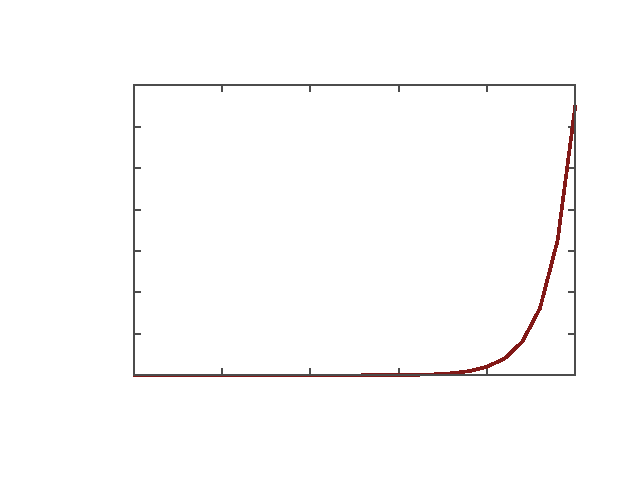
\includegraphics{./graficos/hanoi-linux-O0}}%
    \gplfronttext
  \end{picture}%
\endgroup

\end{center}

\section*{Cálculo de la eficiencia empírica}

Puesto que la eficiencia teórica de cada algoritmo es diferente, no podemos realizar las mediciones para los mismos valores de entrada en todos los algoritmos. Así, los agrupamos según su orden de eficiencia.\\

Para el cálculo de la eficiencia empírica, hemos utilizado un \textit{script} que realiza tantas ejecuciones de cada algoritmo como le indiquemos, tomando como parámetros el valor inicial, el incremento, y el valor final de los datos de entrada.\\

Las gráficas anteriores han sido realizadas a partir de los datos recogidos en las siguientes tablas.

\subsection*{Tablas}


\pgfplotstableread{datos/burbuja_datos/burbuja-linux-O0.dat}\burbujalinuxOCero
\pgfplotstableread{datos/seleccion_datos/seleccion-linux-O0.dat}\seleccionlinuxOCero
\pgfplotstableread{datos/insercion_datos/insercion-linux-O0.dat}\insercionlinuxOCero

\pgfplotstablecreatecol[copy column from table={\burbujalinuxOCero}{[index] 1}] {Burbuja} {\burbujalinuxOCero}
\pgfplotstablecreatecol[copy column from table={\seleccionlinuxOCero}{[index] 1}] {Selección} {\burbujalinuxOCero}
\pgfplotstablecreatecol[copy column from table={\insercionlinuxOCero}{[index] 1}] {Inserción} {\burbujalinuxOCero}

\pgfplotstableread{datos/mergesort_datos/mergesort-linux-O0.dat}\mergesortlinuxOCero
\pgfplotstableread{datos/quicksort_datos/quicksort-linux-O0.dat}\quicksortlinuxOCero
\pgfplotstableread{datos/heapsort_datos/heapsort-linux-O0.dat}\heapsortlinuxOCero

\pgfplotstablecreatecol[copy column from table={\mergesortlinuxOCero}{[index] 1}] {Mergesort} {\mergesortlinuxOCero}
\pgfplotstablecreatecol[copy column from table={\quicksortlinuxOCero}{[index] 1}] {Quicksort} {\mergesortlinuxOCero}
\pgfplotstablecreatecol[copy column from table={\heapsortlinuxOCero}{[index] 1}] {Heapsort} {\mergesortlinuxOCero}

\pgfplotstableread{datos/floyd_datos/floyd-linux-O0.dat}\floydlinuxOCero
\pgfplotstableread{datos/hanoi_datos/hanoi-linux-O0.dat}\hanoilinuxOCero

\pgfplotstablecreatecol[copy column from table={\floydlinuxOCero}{[index] 1}] {Floyd} {\floydlinuxOCero}
\pgfplotstablecreatecol[copy column from table={\hanoilinuxOCero}{[index] 1}] {Hanoi} {\hanoilinuxOCero}

\begin{figure}[H]
	\centering
	\caption*{Algoritmos que son $O(n^2)$ (tiempos en segundos)}
	\pgfplotstabletypeset[columns={0, Burbuja, Selección, Inserción}]{\burbujalinuxOCero}
\end{figure}


\begin{figure}[H]
	\centering
	\caption*{Algoritmos que son $O(nlog(n))$ (tiempos en segundos)}
	\pgfplotstabletypeset[columns={0, Mergesort, Quicksort, Heapsort}]{\mergesortlinuxOCero}
\end{figure}

\begin{figure}[H]
	\centering
	\caption*{Algoritmos que son $O(n^3)$ (tiempos en segundos)}
	\pgfplotstabletypeset[columns={0, Floyd}]{\floydlinuxOCero}
\end{figure}


\begin{figure}[H]
	\centering
	\caption*{Algoritmos que son $O(2^n)$ (tiempos en segundos)}
	\pgfplotstabletypeset[columns={0, Hanoi}]{\hanoilinuxOCero}
\end{figure}


    
\subsection*{Gráficos}

A continuación se muestran los gráficos que corresponden a la comparación de aquellos algoritmos que son de un mismo orden.

\subsubsection*{Algoritmos que son $\boldsymbol{O(n^2}$)}

\begin{center}
	% GNUPLOT: LaTeX picture with Postscript
\begingroup
  \makeatletter
  \providecommand\color[2][]{%
    \GenericError{(gnuplot) \space\space\space\@spaces}{%
      Package color not loaded in conjunction with
      terminal option `colourtext'%
    }{See the gnuplot documentation for explanation.%
    }{Either use 'blacktext' in gnuplot or load the package
      color.sty in LaTeX.}%
    \renewcommand\color[2][]{}%
  }%
  \providecommand\includegraphics[2][]{%
    \GenericError{(gnuplot) \space\space\space\@spaces}{%
      Package graphicx or graphics not loaded%
    }{See the gnuplot documentation for explanation.%
    }{The gnuplot epslatex terminal needs graphicx.sty or graphics.sty.}%
    \renewcommand\includegraphics[2][]{}%
  }%
  \providecommand\rotatebox[2]{#2}%
  \@ifundefined{ifGPcolor}{%
    \newif\ifGPcolor
    \GPcolortrue
  }{}%
  \@ifundefined{ifGPblacktext}{%
    \newif\ifGPblacktext
    \GPblacktextfalse
  }{}%
  % define a \g@addto@macro without @ in the name:
  \let\gplgaddtomacro\g@addto@macro
  % define empty templates for all commands taking text:
  \gdef\gplbacktext{}%
  \gdef\gplfronttext{}%
  \makeatother
  \ifGPblacktext
    % no textcolor at all
    \def\colorrgb#1{}%
    \def\colorgray#1{}%
  \else
    % gray or color?
    \ifGPcolor
      \def\colorrgb#1{\color[rgb]{#1}}%
      \def\colorgray#1{\color[gray]{#1}}%
      \expandafter\def\csname LTw\endcsname{\color{white}}%
      \expandafter\def\csname LTb\endcsname{\color{black}}%
      \expandafter\def\csname LTa\endcsname{\color{black}}%
      \expandafter\def\csname LT0\endcsname{\color[rgb]{1,0,0}}%
      \expandafter\def\csname LT1\endcsname{\color[rgb]{0,1,0}}%
      \expandafter\def\csname LT2\endcsname{\color[rgb]{0,0,1}}%
      \expandafter\def\csname LT3\endcsname{\color[rgb]{1,0,1}}%
      \expandafter\def\csname LT4\endcsname{\color[rgb]{0,1,1}}%
      \expandafter\def\csname LT5\endcsname{\color[rgb]{1,1,0}}%
      \expandafter\def\csname LT6\endcsname{\color[rgb]{0,0,0}}%
      \expandafter\def\csname LT7\endcsname{\color[rgb]{1,0.3,0}}%
      \expandafter\def\csname LT8\endcsname{\color[rgb]{0.5,0.5,0.5}}%
    \else
      % gray
      \def\colorrgb#1{\color{black}}%
      \def\colorgray#1{\color[gray]{#1}}%
      \expandafter\def\csname LTw\endcsname{\color{white}}%
      \expandafter\def\csname LTb\endcsname{\color{black}}%
      \expandafter\def\csname LTa\endcsname{\color{black}}%
      \expandafter\def\csname LT0\endcsname{\color{black}}%
      \expandafter\def\csname LT1\endcsname{\color{black}}%
      \expandafter\def\csname LT2\endcsname{\color{black}}%
      \expandafter\def\csname LT3\endcsname{\color{black}}%
      \expandafter\def\csname LT4\endcsname{\color{black}}%
      \expandafter\def\csname LT5\endcsname{\color{black}}%
      \expandafter\def\csname LT6\endcsname{\color{black}}%
      \expandafter\def\csname LT7\endcsname{\color{black}}%
      \expandafter\def\csname LT8\endcsname{\color{black}}%
    \fi
  \fi
    \setlength{\unitlength}{0.0500bp}%
    \ifx\gptboxheight\undefined%
      \newlength{\gptboxheight}%
      \newlength{\gptboxwidth}%
      \newsavebox{\gptboxtext}%
    \fi%
    \setlength{\fboxrule}{0.5pt}%
    \setlength{\fboxsep}{1pt}%
\begin{picture}(5760.00,4320.00)%
    \gplgaddtomacro\gplbacktext{%
      \colorrgb{0.30,0.30,0.30}%
      \put(990,1153){\makebox(0,0)[r]{\strut{}$\textcolor{text}{0}$}}%
      \colorrgb{0.30,0.30,0.30}%
      \put(990,1466){\makebox(0,0)[r]{\strut{}$\textcolor{text}{1}$}}%
      \colorrgb{0.30,0.30,0.30}%
      \put(990,1780){\makebox(0,0)[r]{\strut{}$\textcolor{text}{2}$}}%
      \colorrgb{0.30,0.30,0.30}%
      \put(990,2093){\makebox(0,0)[r]{\strut{}$\textcolor{text}{3}$}}%
      \colorrgb{0.30,0.30,0.30}%
      \put(990,2406){\makebox(0,0)[r]{\strut{}$\textcolor{text}{4}$}}%
      \colorrgb{0.30,0.30,0.30}%
      \put(990,2719){\makebox(0,0)[r]{\strut{}$\textcolor{text}{5}$}}%
      \colorrgb{0.30,0.30,0.30}%
      \put(990,3033){\makebox(0,0)[r]{\strut{}$\textcolor{text}{6}$}}%
      \colorrgb{0.30,0.30,0.30}%
      \put(990,3346){\makebox(0,0)[r]{\strut{}$\textcolor{text}{7}$}}%
      \colorrgb{0.30,0.30,0.30}%
      \put(990,3659){\makebox(0,0)[r]{\strut{}$\textcolor{text}{8}$}}%
      \colorrgb{0.30,0.30,0.30}%
      \put(1122,1021){\rotatebox{45}{\makebox(0,0)[r]{\strut{}$\textcolor{text}{0}$}}}%
      \colorrgb{0.30,0.30,0.30}%
      \put(1546,1021){\rotatebox{45}{\makebox(0,0)[r]{\strut{}$\textcolor{text}{5000}$}}}%
      \colorrgb{0.30,0.30,0.30}%
      \put(1970,1021){\rotatebox{45}{\makebox(0,0)[r]{\strut{}$\textcolor{text}{10000}$}}}%
      \colorrgb{0.30,0.30,0.30}%
      \put(2394,1021){\rotatebox{45}{\makebox(0,0)[r]{\strut{}$\textcolor{text}{15000}$}}}%
      \colorrgb{0.30,0.30,0.30}%
      \put(2818,1021){\rotatebox{45}{\makebox(0,0)[r]{\strut{}$\textcolor{text}{20000}$}}}%
      \colorrgb{0.30,0.30,0.30}%
      \put(3243,1021){\rotatebox{45}{\makebox(0,0)[r]{\strut{}$\textcolor{text}{25000}$}}}%
      \colorrgb{0.30,0.30,0.30}%
      \put(3667,1021){\rotatebox{45}{\makebox(0,0)[r]{\strut{}$\textcolor{text}{30000}$}}}%
      \colorrgb{0.30,0.30,0.30}%
      \put(4091,1021){\rotatebox{45}{\makebox(0,0)[r]{\strut{}$\textcolor{text}{35000}$}}}%
      \colorrgb{0.30,0.30,0.30}%
      \put(4515,1021){\rotatebox{45}{\makebox(0,0)[r]{\strut{}$\textcolor{text}{40000}$}}}%
      \colorrgb{0.30,0.30,0.30}%
      \put(4939,1021){\rotatebox{45}{\makebox(0,0)[r]{\strut{}$\textcolor{text}{45000}$}}}%
      \colorrgb{0.30,0.30,0.30}%
      \put(5363,1021){\rotatebox{45}{\makebox(0,0)[r]{\strut{}$\textcolor{text}{50000}$}}}%
    }%
    \gplgaddtomacro\gplfronttext{%
      \colorrgb{0.30,0.30,0.30}%
      \put(220,2406){\rotatebox{-270}{\makebox(0,0){\strut{}Tiempo de ejecución (s)}}}%
      \colorrgb{0.30,0.30,0.30}%
      \put(3242,220){\makebox(0,0){\strut{}Tamaño del vector (elementos)}}%
      \colorrgb{0.30,0.30,0.30}%
      \put(3242,3989){\makebox(0,0){\strut{}Algoritmos de ordenación $O(n^2)$}}%
      \csname LTb\endcsname%
      \put(4376,3486){\makebox(0,0)[r]{\strut{}Burbuja}}%
      \csname LTb\endcsname%
      \put(4376,3266){\makebox(0,0)[r]{\strut{}Inserción}}%
      \csname LTb\endcsname%
      \put(4376,3046){\makebox(0,0)[r]{\strut{}Selección}}%
    }%
    \gplbacktext
    \put(0,0){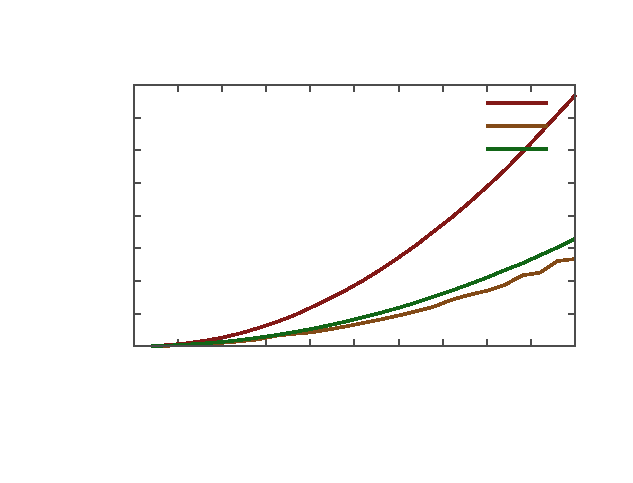
\includegraphics{./graficos/ncuadrado}}%
    \gplfronttext
  \end{picture}%
\endgroup

\end{center}

Observamos que el algoritmo burbuja es claramente más lento para estos valores. Esto se verá reflejado cuando calculemos los valores de las constantes ocultas.


\subsubsection*{Algoritmos que son $\boldsymbol{O(n\log n}$)}

\begin{adjustbox}{center}
	% GNUPLOT: LaTeX picture with Postscript
\begingroup
  \makeatletter
  \providecommand\color[2][]{%
    \GenericError{(gnuplot) \space\space\space\@spaces}{%
      Package color not loaded in conjunction with
      terminal option `colourtext'%
    }{See the gnuplot documentation for explanation.%
    }{Either use 'blacktext' in gnuplot or load the package
      color.sty in LaTeX.}%
    \renewcommand\color[2][]{}%
  }%
  \providecommand\includegraphics[2][]{%
    \GenericError{(gnuplot) \space\space\space\@spaces}{%
      Package graphicx or graphics not loaded%
    }{See the gnuplot documentation for explanation.%
    }{The gnuplot epslatex terminal needs graphicx.sty or graphics.sty.}%
    \renewcommand\includegraphics[2][]{}%
  }%
  \providecommand\rotatebox[2]{#2}%
  \@ifundefined{ifGPcolor}{%
    \newif\ifGPcolor
    \GPcolortrue
  }{}%
  \@ifundefined{ifGPblacktext}{%
    \newif\ifGPblacktext
    \GPblacktextfalse
  }{}%
  % define a \g@addto@macro without @ in the name:
  \let\gplgaddtomacro\g@addto@macro
  % define empty templates for all commands taking text:
  \gdef\gplbacktext{}%
  \gdef\gplfronttext{}%
  \makeatother
  \ifGPblacktext
    % no textcolor at all
    \def\colorrgb#1{}%
    \def\colorgray#1{}%
  \else
    % gray or color?
    \ifGPcolor
      \def\colorrgb#1{\color[rgb]{#1}}%
      \def\colorgray#1{\color[gray]{#1}}%
      \expandafter\def\csname LTw\endcsname{\color{white}}%
      \expandafter\def\csname LTb\endcsname{\color{black}}%
      \expandafter\def\csname LTa\endcsname{\color{black}}%
      \expandafter\def\csname LT0\endcsname{\color[rgb]{1,0,0}}%
      \expandafter\def\csname LT1\endcsname{\color[rgb]{0,1,0}}%
      \expandafter\def\csname LT2\endcsname{\color[rgb]{0,0,1}}%
      \expandafter\def\csname LT3\endcsname{\color[rgb]{1,0,1}}%
      \expandafter\def\csname LT4\endcsname{\color[rgb]{0,1,1}}%
      \expandafter\def\csname LT5\endcsname{\color[rgb]{1,1,0}}%
      \expandafter\def\csname LT6\endcsname{\color[rgb]{0,0,0}}%
      \expandafter\def\csname LT7\endcsname{\color[rgb]{1,0.3,0}}%
      \expandafter\def\csname LT8\endcsname{\color[rgb]{0.5,0.5,0.5}}%
    \else
      % gray
      \def\colorrgb#1{\color{black}}%
      \def\colorgray#1{\color[gray]{#1}}%
      \expandafter\def\csname LTw\endcsname{\color{white}}%
      \expandafter\def\csname LTb\endcsname{\color{black}}%
      \expandafter\def\csname LTa\endcsname{\color{black}}%
      \expandafter\def\csname LT0\endcsname{\color{black}}%
      \expandafter\def\csname LT1\endcsname{\color{black}}%
      \expandafter\def\csname LT2\endcsname{\color{black}}%
      \expandafter\def\csname LT3\endcsname{\color{black}}%
      \expandafter\def\csname LT4\endcsname{\color{black}}%
      \expandafter\def\csname LT5\endcsname{\color{black}}%
      \expandafter\def\csname LT6\endcsname{\color{black}}%
      \expandafter\def\csname LT7\endcsname{\color{black}}%
      \expandafter\def\csname LT8\endcsname{\color{black}}%
    \fi
  \fi
    \setlength{\unitlength}{0.0500bp}%
    \ifx\gptboxheight\undefined%
      \newlength{\gptboxheight}%
      \newlength{\gptboxwidth}%
      \newsavebox{\gptboxtext}%
    \fi%
    \setlength{\fboxrule}{0.5pt}%
    \setlength{\fboxsep}{1pt}%
\begin{picture}(5760.00,4320.00)%
    \gplgaddtomacro\gplbacktext{%
      \colorrgb{0.30,0.30,0.30}%
      \put(1650,1246){\makebox(0,0)[r]{\strut{}$\textcolor{text}{0.0001}$}}%
      \colorrgb{0.30,0.30,0.30}%
      \put(1650,2050){\makebox(0,0)[r]{\strut{}$\textcolor{text}{0.001}$}}%
      \colorrgb{0.30,0.30,0.30}%
      \put(1650,2855){\makebox(0,0)[r]{\strut{}$\textcolor{text}{0.01}$}}%
      \colorrgb{0.30,0.30,0.30}%
      \put(1650,3659){\makebox(0,0)[r]{\strut{}$\textcolor{text}{0.1}$}}%
      \colorrgb{0.30,0.30,0.30}%
      \put(1782,1114){\rotatebox{45}{\makebox(0,0)[r]{\strut{}$\textcolor{text}{0}$}}}%
      \colorrgb{0.30,0.30,0.30}%
      \put(2230,1114){\rotatebox{45}{\makebox(0,0)[r]{\strut{}$\textcolor{text}{20000}$}}}%
      \colorrgb{0.30,0.30,0.30}%
      \put(2677,1114){\rotatebox{45}{\makebox(0,0)[r]{\strut{}$\textcolor{text}{40000}$}}}%
      \colorrgb{0.30,0.30,0.30}%
      \put(3125,1114){\rotatebox{45}{\makebox(0,0)[r]{\strut{}$\textcolor{text}{60000}$}}}%
      \colorrgb{0.30,0.30,0.30}%
      \put(3573,1114){\rotatebox{45}{\makebox(0,0)[r]{\strut{}$\textcolor{text}{80000}$}}}%
      \colorrgb{0.30,0.30,0.30}%
      \put(4020,1114){\rotatebox{45}{\makebox(0,0)[r]{\strut{}$\textcolor{text}{100000}$}}}%
      \colorrgb{0.30,0.30,0.30}%
      \put(4468,1114){\rotatebox{45}{\makebox(0,0)[r]{\strut{}$\textcolor{text}{120000}$}}}%
      \colorrgb{0.30,0.30,0.30}%
      \put(4915,1114){\rotatebox{45}{\makebox(0,0)[r]{\strut{}$\textcolor{text}{140000}$}}}%
      \colorrgb{0.30,0.30,0.30}%
      \put(5363,1114){\rotatebox{45}{\makebox(0,0)[r]{\strut{}$\textcolor{text}{160000}$}}}%
    }%
    \gplgaddtomacro\gplfronttext{%
      \colorrgb{0.30,0.30,0.30}%
      \put(220,2452){\rotatebox{-270}{\makebox(0,0){\strut{}Tiempo de ejecución (s)}}}%
      \colorrgb{0.30,0.30,0.30}%
      \put(3572,220){\makebox(0,0){\strut{}Tamaño del vector (elementos)}}%
      \colorrgb{0.30,0.30,0.30}%
      \put(3572,3989){\makebox(0,0){\strut{}Algoritmos de ordenación $O(nlogn)$}}%
      \csname LTb\endcsname%
      \put(4376,3486){\makebox(0,0)[r]{\strut{}Mergesort}}%
      \csname LTb\endcsname%
      \put(4376,3266){\makebox(0,0)[r]{\strut{}Heapsort}}%
      \csname LTb\endcsname%
      \put(4376,3046){\makebox(0,0)[r]{\strut{}Quicksort}}%
    }%
    \gplbacktext
    \put(0,0){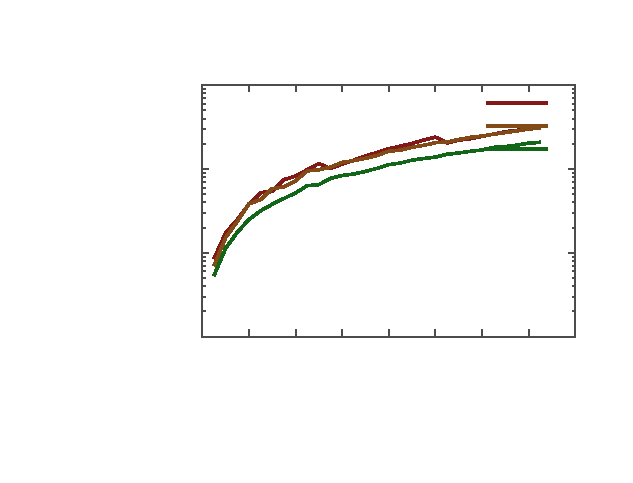
\includegraphics{./graficos/nlogn}}%
    \gplfronttext
  \end{picture}%
\endgroup

\end{adjustbox}

Estos algoritmos se ejecutan en tiempos similares, aunque quicksort es ligeramente más rápido, manteniendo de forma uniforme la diferencia con los otros dos algoritmos a medida que aumenta el número de valores.

\subsubsection*{Algoritmos de ordenación}

\begin{adjustbox}{center}
	% GNUPLOT: LaTeX picture with Postscript
\begingroup
  \makeatletter
  \providecommand\color[2][]{%
    \GenericError{(gnuplot) \space\space\space\@spaces}{%
      Package color not loaded in conjunction with
      terminal option `colourtext'%
    }{See the gnuplot documentation for explanation.%
    }{Either use 'blacktext' in gnuplot or load the package
      color.sty in LaTeX.}%
    \renewcommand\color[2][]{}%
  }%
  \providecommand\includegraphics[2][]{%
    \GenericError{(gnuplot) \space\space\space\@spaces}{%
      Package graphicx or graphics not loaded%
    }{See the gnuplot documentation for explanation.%
    }{The gnuplot epslatex terminal needs graphicx.sty or graphics.sty.}%
    \renewcommand\includegraphics[2][]{}%
  }%
  \providecommand\rotatebox[2]{#2}%
  \@ifundefined{ifGPcolor}{%
    \newif\ifGPcolor
    \GPcolortrue
  }{}%
  \@ifundefined{ifGPblacktext}{%
    \newif\ifGPblacktext
    \GPblacktextfalse
  }{}%
  % define a \g@addto@macro without @ in the name:
  \let\gplgaddtomacro\g@addto@macro
  % define empty templates for all commands taking text:
  \gdef\gplbacktext{}%
  \gdef\gplfronttext{}%
  \makeatother
  \ifGPblacktext
    % no textcolor at all
    \def\colorrgb#1{}%
    \def\colorgray#1{}%
  \else
    % gray or color?
    \ifGPcolor
      \def\colorrgb#1{\color[rgb]{#1}}%
      \def\colorgray#1{\color[gray]{#1}}%
      \expandafter\def\csname LTw\endcsname{\color{white}}%
      \expandafter\def\csname LTb\endcsname{\color{black}}%
      \expandafter\def\csname LTa\endcsname{\color{black}}%
      \expandafter\def\csname LT0\endcsname{\color[rgb]{1,0,0}}%
      \expandafter\def\csname LT1\endcsname{\color[rgb]{0,1,0}}%
      \expandafter\def\csname LT2\endcsname{\color[rgb]{0,0,1}}%
      \expandafter\def\csname LT3\endcsname{\color[rgb]{1,0,1}}%
      \expandafter\def\csname LT4\endcsname{\color[rgb]{0,1,1}}%
      \expandafter\def\csname LT5\endcsname{\color[rgb]{1,1,0}}%
      \expandafter\def\csname LT6\endcsname{\color[rgb]{0,0,0}}%
      \expandafter\def\csname LT7\endcsname{\color[rgb]{1,0.3,0}}%
      \expandafter\def\csname LT8\endcsname{\color[rgb]{0.5,0.5,0.5}}%
    \else
      % gray
      \def\colorrgb#1{\color{black}}%
      \def\colorgray#1{\color[gray]{#1}}%
      \expandafter\def\csname LTw\endcsname{\color{white}}%
      \expandafter\def\csname LTb\endcsname{\color{black}}%
      \expandafter\def\csname LTa\endcsname{\color{black}}%
      \expandafter\def\csname LT0\endcsname{\color{black}}%
      \expandafter\def\csname LT1\endcsname{\color{black}}%
      \expandafter\def\csname LT2\endcsname{\color{black}}%
      \expandafter\def\csname LT3\endcsname{\color{black}}%
      \expandafter\def\csname LT4\endcsname{\color{black}}%
      \expandafter\def\csname LT5\endcsname{\color{black}}%
      \expandafter\def\csname LT6\endcsname{\color{black}}%
      \expandafter\def\csname LT7\endcsname{\color{black}}%
      \expandafter\def\csname LT8\endcsname{\color{black}}%
    \fi
  \fi
    \setlength{\unitlength}{0.0500bp}%
    \ifx\gptboxheight\undefined%
      \newlength{\gptboxheight}%
      \newlength{\gptboxwidth}%
      \newsavebox{\gptboxtext}%
    \fi%
    \setlength{\fboxrule}{0.5pt}%
    \setlength{\fboxsep}{1pt}%
\begin{picture}(5760.00,4320.00)%
    \gplgaddtomacro\gplbacktext{%
      \colorrgb{0.30,0.30,0.30}%
      \put(1650,1246){\makebox(0,0)[r]{\strut{}$\textcolor{text}{0.0001}$}}%
      \colorrgb{0.30,0.30,0.30}%
      \put(1650,1648){\makebox(0,0)[r]{\strut{}$\textcolor{text}{0.001}$}}%
      \colorrgb{0.30,0.30,0.30}%
      \put(1650,2050){\makebox(0,0)[r]{\strut{}$\textcolor{text}{0.01}$}}%
      \colorrgb{0.30,0.30,0.30}%
      \put(1650,2453){\makebox(0,0)[r]{\strut{}$\textcolor{text}{0.1}$}}%
      \colorrgb{0.30,0.30,0.30}%
      \put(1650,2855){\makebox(0,0)[r]{\strut{}$\textcolor{text}{1}$}}%
      \colorrgb{0.30,0.30,0.30}%
      \put(1650,3257){\makebox(0,0)[r]{\strut{}$\textcolor{text}{10}$}}%
      \colorrgb{0.30,0.30,0.30}%
      \put(1650,3659){\makebox(0,0)[r]{\strut{}$\textcolor{text}{100}$}}%
      \colorrgb{0.30,0.30,0.30}%
      \put(1782,1114){\rotatebox{45}{\makebox(0,0)[r]{\strut{}$\textcolor{text}{0}$}}}%
      \colorrgb{0.30,0.30,0.30}%
      \put(2230,1114){\rotatebox{45}{\makebox(0,0)[r]{\strut{}$\textcolor{text}{20000}$}}}%
      \colorrgb{0.30,0.30,0.30}%
      \put(2677,1114){\rotatebox{45}{\makebox(0,0)[r]{\strut{}$\textcolor{text}{40000}$}}}%
      \colorrgb{0.30,0.30,0.30}%
      \put(3125,1114){\rotatebox{45}{\makebox(0,0)[r]{\strut{}$\textcolor{text}{60000}$}}}%
      \colorrgb{0.30,0.30,0.30}%
      \put(3573,1114){\rotatebox{45}{\makebox(0,0)[r]{\strut{}$\textcolor{text}{80000}$}}}%
      \colorrgb{0.30,0.30,0.30}%
      \put(4020,1114){\rotatebox{45}{\makebox(0,0)[r]{\strut{}$\textcolor{text}{100000}$}}}%
      \colorrgb{0.30,0.30,0.30}%
      \put(4468,1114){\rotatebox{45}{\makebox(0,0)[r]{\strut{}$\textcolor{text}{120000}$}}}%
      \colorrgb{0.30,0.30,0.30}%
      \put(4915,1114){\rotatebox{45}{\makebox(0,0)[r]{\strut{}$\textcolor{text}{140000}$}}}%
      \colorrgb{0.30,0.30,0.30}%
      \put(5363,1114){\rotatebox{45}{\makebox(0,0)[r]{\strut{}$\textcolor{text}{160000}$}}}%
    }%
    \gplgaddtomacro\gplfronttext{%
      \colorrgb{0.30,0.30,0.30}%
      \put(220,2452){\rotatebox{-270}{\makebox(0,0){\strut{}Tiempo de ejecución (s)}}}%
      \colorrgb{0.30,0.30,0.30}%
      \put(3572,220){\makebox(0,0){\strut{}Tamaño del vector (elementos)}}%
      \colorrgb{0.30,0.30,0.30}%
      \put(3572,3989){\makebox(0,0){\strut{}Algoritmos de ordenación}}%
      \csname LTb\endcsname%
      \put(4376,3486){\makebox(0,0)[r]{\strut{}Mergesort}}%
      \csname LTb\endcsname%
      \put(4376,3266){\makebox(0,0)[r]{\strut{}Heapsort}}%
      \csname LTb\endcsname%
      \put(4376,3046){\makebox(0,0)[r]{\strut{}Quicksort}}%
      \csname LTb\endcsname%
      \put(4376,2826){\makebox(0,0)[r]{\strut{}Burbuja}}%
      \csname LTb\endcsname%
      \put(4376,2606){\makebox(0,0)[r]{\strut{}Inserción}}%
      \csname LTb\endcsname%
      \put(4376,2386){\makebox(0,0)[r]{\strut{}Selección}}%
    }%
    \gplbacktext
    \put(0,0){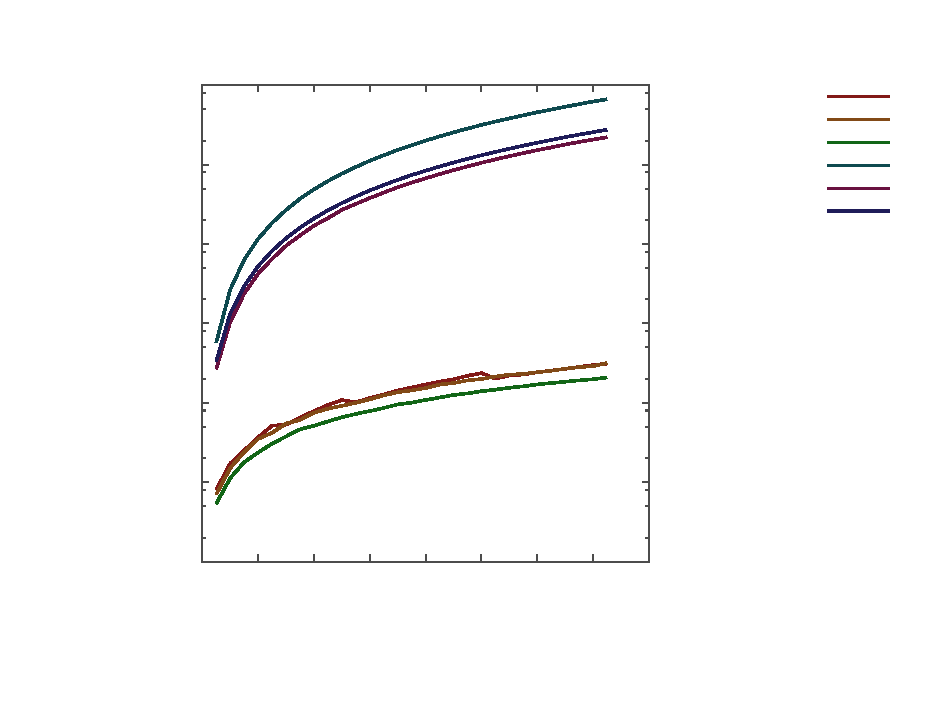
\includegraphics{./graficos/ordenacion}}%
    \gplfronttext
  \end{picture}%
\endgroup

\end{adjustbox}

En este último gráfico, puede observarse claramente la tendencia de los algoritmos cuyo orden de eficiencia es $O(n\log n)$ a ser más rápidos que aquellos que son $O(n^2)$. Se ha utilizado una escala logarítmica para poder representar todos los algoritmos en un mismo gráfico.

\newpage



\section*{Cálculo de la eficiencia híbrida}
A continuación se recogen los gráficos que muestran tanto la eficiencia empírica como la función ajustada o \textit{eficiencia híbrida} de cada algoritmo.



\subsection*{Eficiencia $\boldsymbol{n^2}$}

Para ajustar las algoritmos de ordenación hemos usado una función $f(x)$ de la forma: $f(x) = a_0x^2 + a_1x + a_2$ y con ayuda de gnuplot hemos calculado los valores de las constantes ocultas. 

\begin{center}
	% GNUPLOT: LaTeX picture with Postscript
\begingroup
  \makeatletter
  \providecommand\color[2][]{%
    \GenericError{(gnuplot) \space\space\space\@spaces}{%
      Package color not loaded in conjunction with
      terminal option `colourtext'%
    }{See the gnuplot documentation for explanation.%
    }{Either use 'blacktext' in gnuplot or load the package
      color.sty in LaTeX.}%
    \renewcommand\color[2][]{}%
  }%
  \providecommand\includegraphics[2][]{%
    \GenericError{(gnuplot) \space\space\space\@spaces}{%
      Package graphicx or graphics not loaded%
    }{See the gnuplot documentation for explanation.%
    }{The gnuplot epslatex terminal needs graphicx.sty or graphics.sty.}%
    \renewcommand\includegraphics[2][]{}%
  }%
  \providecommand\rotatebox[2]{#2}%
  \@ifundefined{ifGPcolor}{%
    \newif\ifGPcolor
    \GPcolortrue
  }{}%
  \@ifundefined{ifGPblacktext}{%
    \newif\ifGPblacktext
    \GPblacktextfalse
  }{}%
  % define a \g@addto@macro without @ in the name:
  \let\gplgaddtomacro\g@addto@macro
  % define empty templates for all commands taking text:
  \gdef\gplbacktext{}%
  \gdef\gplfronttext{}%
  \makeatother
  \ifGPblacktext
    % no textcolor at all
    \def\colorrgb#1{}%
    \def\colorgray#1{}%
  \else
    % gray or color?
    \ifGPcolor
      \def\colorrgb#1{\color[rgb]{#1}}%
      \def\colorgray#1{\color[gray]{#1}}%
      \expandafter\def\csname LTw\endcsname{\color{white}}%
      \expandafter\def\csname LTb\endcsname{\color{black}}%
      \expandafter\def\csname LTa\endcsname{\color{black}}%
      \expandafter\def\csname LT0\endcsname{\color[rgb]{1,0,0}}%
      \expandafter\def\csname LT1\endcsname{\color[rgb]{0,1,0}}%
      \expandafter\def\csname LT2\endcsname{\color[rgb]{0,0,1}}%
      \expandafter\def\csname LT3\endcsname{\color[rgb]{1,0,1}}%
      \expandafter\def\csname LT4\endcsname{\color[rgb]{0,1,1}}%
      \expandafter\def\csname LT5\endcsname{\color[rgb]{1,1,0}}%
      \expandafter\def\csname LT6\endcsname{\color[rgb]{0,0,0}}%
      \expandafter\def\csname LT7\endcsname{\color[rgb]{1,0.3,0}}%
      \expandafter\def\csname LT8\endcsname{\color[rgb]{0.5,0.5,0.5}}%
    \else
      % gray
      \def\colorrgb#1{\color{black}}%
      \def\colorgray#1{\color[gray]{#1}}%
      \expandafter\def\csname LTw\endcsname{\color{white}}%
      \expandafter\def\csname LTb\endcsname{\color{black}}%
      \expandafter\def\csname LTa\endcsname{\color{black}}%
      \expandafter\def\csname LT0\endcsname{\color{black}}%
      \expandafter\def\csname LT1\endcsname{\color{black}}%
      \expandafter\def\csname LT2\endcsname{\color{black}}%
      \expandafter\def\csname LT3\endcsname{\color{black}}%
      \expandafter\def\csname LT4\endcsname{\color{black}}%
      \expandafter\def\csname LT5\endcsname{\color{black}}%
      \expandafter\def\csname LT6\endcsname{\color{black}}%
      \expandafter\def\csname LT7\endcsname{\color{black}}%
      \expandafter\def\csname LT8\endcsname{\color{black}}%
    \fi
  \fi
    \setlength{\unitlength}{0.0500bp}%
    \ifx\gptboxheight\undefined%
      \newlength{\gptboxheight}%
      \newlength{\gptboxwidth}%
      \newsavebox{\gptboxtext}%
    \fi%
    \setlength{\fboxrule}{0.5pt}%
    \setlength{\fboxsep}{1pt}%
\begin{picture}(5760.00,4320.00)%
    \gplgaddtomacro\gplbacktext{%
      \colorrgb{0.30,0.30,0.30}%
      \put(990,1153){\makebox(0,0)[r]{\strut{}$\textcolor{text}{0}$}}%
      \colorrgb{0.30,0.30,0.30}%
      \put(990,1466){\makebox(0,0)[r]{\strut{}$\textcolor{text}{1}$}}%
      \colorrgb{0.30,0.30,0.30}%
      \put(990,1780){\makebox(0,0)[r]{\strut{}$\textcolor{text}{2}$}}%
      \colorrgb{0.30,0.30,0.30}%
      \put(990,2093){\makebox(0,0)[r]{\strut{}$\textcolor{text}{3}$}}%
      \colorrgb{0.30,0.30,0.30}%
      \put(990,2406){\makebox(0,0)[r]{\strut{}$\textcolor{text}{4}$}}%
      \colorrgb{0.30,0.30,0.30}%
      \put(990,2719){\makebox(0,0)[r]{\strut{}$\textcolor{text}{5}$}}%
      \colorrgb{0.30,0.30,0.30}%
      \put(990,3033){\makebox(0,0)[r]{\strut{}$\textcolor{text}{6}$}}%
      \colorrgb{0.30,0.30,0.30}%
      \put(990,3346){\makebox(0,0)[r]{\strut{}$\textcolor{text}{7}$}}%
      \colorrgb{0.30,0.30,0.30}%
      \put(990,3659){\makebox(0,0)[r]{\strut{}$\textcolor{text}{8}$}}%
      \colorrgb{0.30,0.30,0.30}%
      \put(1122,1021){\rotatebox{45}{\makebox(0,0)[r]{\strut{}$\textcolor{text}{0}$}}}%
      \colorrgb{0.30,0.30,0.30}%
      \put(1546,1021){\rotatebox{45}{\makebox(0,0)[r]{\strut{}$\textcolor{text}{5000}$}}}%
      \colorrgb{0.30,0.30,0.30}%
      \put(1970,1021){\rotatebox{45}{\makebox(0,0)[r]{\strut{}$\textcolor{text}{10000}$}}}%
      \colorrgb{0.30,0.30,0.30}%
      \put(2394,1021){\rotatebox{45}{\makebox(0,0)[r]{\strut{}$\textcolor{text}{15000}$}}}%
      \colorrgb{0.30,0.30,0.30}%
      \put(2818,1021){\rotatebox{45}{\makebox(0,0)[r]{\strut{}$\textcolor{text}{20000}$}}}%
      \colorrgb{0.30,0.30,0.30}%
      \put(3243,1021){\rotatebox{45}{\makebox(0,0)[r]{\strut{}$\textcolor{text}{25000}$}}}%
      \colorrgb{0.30,0.30,0.30}%
      \put(3667,1021){\rotatebox{45}{\makebox(0,0)[r]{\strut{}$\textcolor{text}{30000}$}}}%
      \colorrgb{0.30,0.30,0.30}%
      \put(4091,1021){\rotatebox{45}{\makebox(0,0)[r]{\strut{}$\textcolor{text}{35000}$}}}%
      \colorrgb{0.30,0.30,0.30}%
      \put(4515,1021){\rotatebox{45}{\makebox(0,0)[r]{\strut{}$\textcolor{text}{40000}$}}}%
      \colorrgb{0.30,0.30,0.30}%
      \put(4939,1021){\rotatebox{45}{\makebox(0,0)[r]{\strut{}$\textcolor{text}{45000}$}}}%
      \colorrgb{0.30,0.30,0.30}%
      \put(5363,1021){\rotatebox{45}{\makebox(0,0)[r]{\strut{}$\textcolor{text}{50000}$}}}%
    }%
    \gplgaddtomacro\gplfronttext{%
      \colorrgb{0.30,0.30,0.30}%
      \put(220,2406){\rotatebox{-270}{\makebox(0,0){\strut{}Tiempo de ejecución (s)}}}%
      \colorrgb{0.30,0.30,0.30}%
      \put(3242,220){\makebox(0,0){\strut{}Tamaño del vector (elementos)}}%
      \colorrgb{0.30,0.30,0.30}%
      \put(3242,3989){\makebox(0,0){\strut{}Ajuste Burbuja}}%
      \csname LTb\endcsname%
      \put(4376,3486){\makebox(0,0)[r]{\strut{}3.19e-09$x^2$+-5.20e-06$x$+5.81e-04}}%
      \csname LTb\endcsname%
      \put(4376,3266){\makebox(0,0)[r]{\strut{}Burbuja}}%
    }%
    \gplbacktext
    \put(0,0){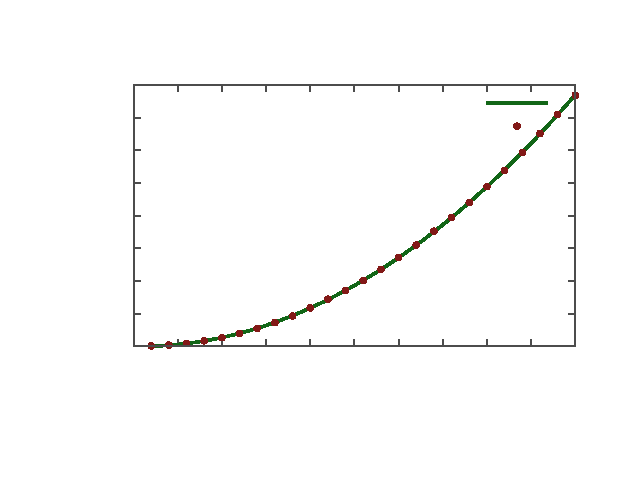
\includegraphics{./graficos/ajuste-burbuja}}%
    \gplfronttext
  \end{picture}%
\endgroup

\end{center}

\begin{center}
	% GNUPLOT: LaTeX picture with Postscript
\begingroup
  \makeatletter
  \providecommand\color[2][]{%
    \GenericError{(gnuplot) \space\space\space\@spaces}{%
      Package color not loaded in conjunction with
      terminal option `colourtext'%
    }{See the gnuplot documentation for explanation.%
    }{Either use 'blacktext' in gnuplot or load the package
      color.sty in LaTeX.}%
    \renewcommand\color[2][]{}%
  }%
  \providecommand\includegraphics[2][]{%
    \GenericError{(gnuplot) \space\space\space\@spaces}{%
      Package graphicx or graphics not loaded%
    }{See the gnuplot documentation for explanation.%
    }{The gnuplot epslatex terminal needs graphicx.sty or graphics.sty.}%
    \renewcommand\includegraphics[2][]{}%
  }%
  \providecommand\rotatebox[2]{#2}%
  \@ifundefined{ifGPcolor}{%
    \newif\ifGPcolor
    \GPcolortrue
  }{}%
  \@ifundefined{ifGPblacktext}{%
    \newif\ifGPblacktext
    \GPblacktextfalse
  }{}%
  % define a \g@addto@macro without @ in the name:
  \let\gplgaddtomacro\g@addto@macro
  % define empty templates for all commands taking text:
  \gdef\gplbacktext{}%
  \gdef\gplfronttext{}%
  \makeatother
  \ifGPblacktext
    % no textcolor at all
    \def\colorrgb#1{}%
    \def\colorgray#1{}%
  \else
    % gray or color?
    \ifGPcolor
      \def\colorrgb#1{\color[rgb]{#1}}%
      \def\colorgray#1{\color[gray]{#1}}%
      \expandafter\def\csname LTw\endcsname{\color{white}}%
      \expandafter\def\csname LTb\endcsname{\color{black}}%
      \expandafter\def\csname LTa\endcsname{\color{black}}%
      \expandafter\def\csname LT0\endcsname{\color[rgb]{1,0,0}}%
      \expandafter\def\csname LT1\endcsname{\color[rgb]{0,1,0}}%
      \expandafter\def\csname LT2\endcsname{\color[rgb]{0,0,1}}%
      \expandafter\def\csname LT3\endcsname{\color[rgb]{1,0,1}}%
      \expandafter\def\csname LT4\endcsname{\color[rgb]{0,1,1}}%
      \expandafter\def\csname LT5\endcsname{\color[rgb]{1,1,0}}%
      \expandafter\def\csname LT6\endcsname{\color[rgb]{0,0,0}}%
      \expandafter\def\csname LT7\endcsname{\color[rgb]{1,0.3,0}}%
      \expandafter\def\csname LT8\endcsname{\color[rgb]{0.5,0.5,0.5}}%
    \else
      % gray
      \def\colorrgb#1{\color{black}}%
      \def\colorgray#1{\color[gray]{#1}}%
      \expandafter\def\csname LTw\endcsname{\color{white}}%
      \expandafter\def\csname LTb\endcsname{\color{black}}%
      \expandafter\def\csname LTa\endcsname{\color{black}}%
      \expandafter\def\csname LT0\endcsname{\color{black}}%
      \expandafter\def\csname LT1\endcsname{\color{black}}%
      \expandafter\def\csname LT2\endcsname{\color{black}}%
      \expandafter\def\csname LT3\endcsname{\color{black}}%
      \expandafter\def\csname LT4\endcsname{\color{black}}%
      \expandafter\def\csname LT5\endcsname{\color{black}}%
      \expandafter\def\csname LT6\endcsname{\color{black}}%
      \expandafter\def\csname LT7\endcsname{\color{black}}%
      \expandafter\def\csname LT8\endcsname{\color{black}}%
    \fi
  \fi
    \setlength{\unitlength}{0.0500bp}%
    \ifx\gptboxheight\undefined%
      \newlength{\gptboxheight}%
      \newlength{\gptboxwidth}%
      \newsavebox{\gptboxtext}%
    \fi%
    \setlength{\fboxrule}{0.5pt}%
    \setlength{\fboxsep}{1pt}%
\begin{picture}(5760.00,4320.00)%
    \gplgaddtomacro\gplbacktext{%
      \colorrgb{0.30,0.30,0.30}%
      \put(1254,1153){\makebox(0,0)[r]{\strut{}$\textcolor{text}{0}$}}%
      \colorrgb{0.30,0.30,0.30}%
      \put(1254,1571){\makebox(0,0)[r]{\strut{}$\textcolor{text}{0.5}$}}%
      \colorrgb{0.30,0.30,0.30}%
      \put(1254,1988){\makebox(0,0)[r]{\strut{}$\textcolor{text}{1}$}}%
      \colorrgb{0.30,0.30,0.30}%
      \put(1254,2406){\makebox(0,0)[r]{\strut{}$\textcolor{text}{1.5}$}}%
      \colorrgb{0.30,0.30,0.30}%
      \put(1254,2824){\makebox(0,0)[r]{\strut{}$\textcolor{text}{2}$}}%
      \colorrgb{0.30,0.30,0.30}%
      \put(1254,3241){\makebox(0,0)[r]{\strut{}$\textcolor{text}{2.5}$}}%
      \colorrgb{0.30,0.30,0.30}%
      \put(1254,3659){\makebox(0,0)[r]{\strut{}$\textcolor{text}{3}$}}%
      \colorrgb{0.30,0.30,0.30}%
      \put(1386,1021){\rotatebox{45}{\makebox(0,0)[r]{\strut{}$\textcolor{text}{0}$}}}%
      \colorrgb{0.30,0.30,0.30}%
      \put(1784,1021){\rotatebox{45}{\makebox(0,0)[r]{\strut{}$\textcolor{text}{5000}$}}}%
      \colorrgb{0.30,0.30,0.30}%
      \put(2181,1021){\rotatebox{45}{\makebox(0,0)[r]{\strut{}$\textcolor{text}{10000}$}}}%
      \colorrgb{0.30,0.30,0.30}%
      \put(2579,1021){\rotatebox{45}{\makebox(0,0)[r]{\strut{}$\textcolor{text}{15000}$}}}%
      \colorrgb{0.30,0.30,0.30}%
      \put(2977,1021){\rotatebox{45}{\makebox(0,0)[r]{\strut{}$\textcolor{text}{20000}$}}}%
      \colorrgb{0.30,0.30,0.30}%
      \put(3375,1021){\rotatebox{45}{\makebox(0,0)[r]{\strut{}$\textcolor{text}{25000}$}}}%
      \colorrgb{0.30,0.30,0.30}%
      \put(3772,1021){\rotatebox{45}{\makebox(0,0)[r]{\strut{}$\textcolor{text}{30000}$}}}%
      \colorrgb{0.30,0.30,0.30}%
      \put(4170,1021){\rotatebox{45}{\makebox(0,0)[r]{\strut{}$\textcolor{text}{35000}$}}}%
      \colorrgb{0.30,0.30,0.30}%
      \put(4568,1021){\rotatebox{45}{\makebox(0,0)[r]{\strut{}$\textcolor{text}{40000}$}}}%
      \colorrgb{0.30,0.30,0.30}%
      \put(4965,1021){\rotatebox{45}{\makebox(0,0)[r]{\strut{}$\textcolor{text}{45000}$}}}%
      \colorrgb{0.30,0.30,0.30}%
      \put(5363,1021){\rotatebox{45}{\makebox(0,0)[r]{\strut{}$\textcolor{text}{50000}$}}}%
    }%
    \gplgaddtomacro\gplfronttext{%
      \colorrgb{0.30,0.30,0.30}%
      \put(220,2406){\rotatebox{-270}{\makebox(0,0){\strut{}Tiempo de ejecución (s)}}}%
      \colorrgb{0.30,0.30,0.30}%
      \put(3374,220){\makebox(0,0){\strut{}Tamaño del vector (elementos)}}%
      \colorrgb{0.30,0.30,0.30}%
      \put(3374,3989){\makebox(0,0){\strut{}Ajuste Inserción}}%
      \csname LTb\endcsname%
      \put(4376,3486){\makebox(0,0)[r]{\strut{}1.14e-09$x^2$+-2.64e-06$x$+1.87e-02}}%
      \csname LTb\endcsname%
      \put(4376,3266){\makebox(0,0)[r]{\strut{}Inserción}}%
    }%
    \gplbacktext
    \put(0,0){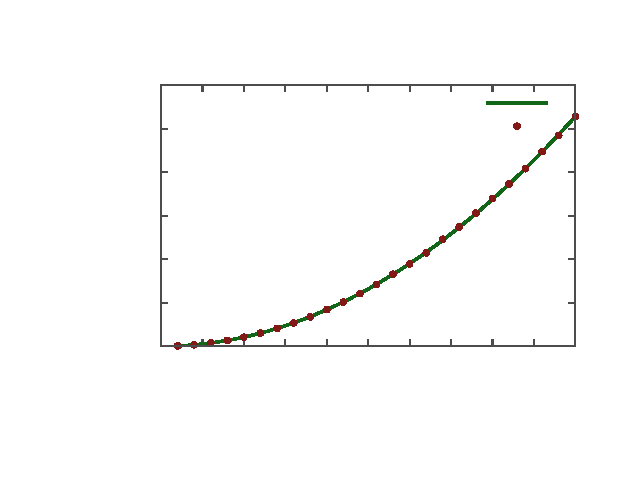
\includegraphics{./graficos/ajuste-insercion}}%
    \gplfronttext
  \end{picture}%
\endgroup

\end{center}

\begin{center}
	% GNUPLOT: LaTeX picture with Postscript
\begingroup
  \makeatletter
  \providecommand\color[2][]{%
    \GenericError{(gnuplot) \space\space\space\@spaces}{%
      Package color not loaded in conjunction with
      terminal option `colourtext'%
    }{See the gnuplot documentation for explanation.%
    }{Either use 'blacktext' in gnuplot or load the package
      color.sty in LaTeX.}%
    \renewcommand\color[2][]{}%
  }%
  \providecommand\includegraphics[2][]{%
    \GenericError{(gnuplot) \space\space\space\@spaces}{%
      Package graphicx or graphics not loaded%
    }{See the gnuplot documentation for explanation.%
    }{The gnuplot epslatex terminal needs graphicx.sty or graphics.sty.}%
    \renewcommand\includegraphics[2][]{}%
  }%
  \providecommand\rotatebox[2]{#2}%
  \@ifundefined{ifGPcolor}{%
    \newif\ifGPcolor
    \GPcolortrue
  }{}%
  \@ifundefined{ifGPblacktext}{%
    \newif\ifGPblacktext
    \GPblacktextfalse
  }{}%
  % define a \g@addto@macro without @ in the name:
  \let\gplgaddtomacro\g@addto@macro
  % define empty templates for all commands taking text:
  \gdef\gplbacktext{}%
  \gdef\gplfronttext{}%
  \makeatother
  \ifGPblacktext
    % no textcolor at all
    \def\colorrgb#1{}%
    \def\colorgray#1{}%
  \else
    % gray or color?
    \ifGPcolor
      \def\colorrgb#1{\color[rgb]{#1}}%
      \def\colorgray#1{\color[gray]{#1}}%
      \expandafter\def\csname LTw\endcsname{\color{white}}%
      \expandafter\def\csname LTb\endcsname{\color{black}}%
      \expandafter\def\csname LTa\endcsname{\color{black}}%
      \expandafter\def\csname LT0\endcsname{\color[rgb]{1,0,0}}%
      \expandafter\def\csname LT1\endcsname{\color[rgb]{0,1,0}}%
      \expandafter\def\csname LT2\endcsname{\color[rgb]{0,0,1}}%
      \expandafter\def\csname LT3\endcsname{\color[rgb]{1,0,1}}%
      \expandafter\def\csname LT4\endcsname{\color[rgb]{0,1,1}}%
      \expandafter\def\csname LT5\endcsname{\color[rgb]{1,1,0}}%
      \expandafter\def\csname LT6\endcsname{\color[rgb]{0,0,0}}%
      \expandafter\def\csname LT7\endcsname{\color[rgb]{1,0.3,0}}%
      \expandafter\def\csname LT8\endcsname{\color[rgb]{0.5,0.5,0.5}}%
    \else
      % gray
      \def\colorrgb#1{\color{black}}%
      \def\colorgray#1{\color[gray]{#1}}%
      \expandafter\def\csname LTw\endcsname{\color{white}}%
      \expandafter\def\csname LTb\endcsname{\color{black}}%
      \expandafter\def\csname LTa\endcsname{\color{black}}%
      \expandafter\def\csname LT0\endcsname{\color{black}}%
      \expandafter\def\csname LT1\endcsname{\color{black}}%
      \expandafter\def\csname LT2\endcsname{\color{black}}%
      \expandafter\def\csname LT3\endcsname{\color{black}}%
      \expandafter\def\csname LT4\endcsname{\color{black}}%
      \expandafter\def\csname LT5\endcsname{\color{black}}%
      \expandafter\def\csname LT6\endcsname{\color{black}}%
      \expandafter\def\csname LT7\endcsname{\color{black}}%
      \expandafter\def\csname LT8\endcsname{\color{black}}%
    \fi
  \fi
    \setlength{\unitlength}{0.0500bp}%
    \ifx\gptboxheight\undefined%
      \newlength{\gptboxheight}%
      \newlength{\gptboxwidth}%
      \newsavebox{\gptboxtext}%
    \fi%
    \setlength{\fboxrule}{0.5pt}%
    \setlength{\fboxsep}{1pt}%
\begin{picture}(5760.00,4320.00)%
    \gplgaddtomacro\gplbacktext{%
      \colorrgb{0.30,0.30,0.30}%
      \put(1254,1153){\makebox(0,0)[r]{\strut{}$\textcolor{text}{0}$}}%
      \colorrgb{0.30,0.30,0.30}%
      \put(1254,1511){\makebox(0,0)[r]{\strut{}$\textcolor{text}{0.5}$}}%
      \colorrgb{0.30,0.30,0.30}%
      \put(1254,1869){\makebox(0,0)[r]{\strut{}$\textcolor{text}{1}$}}%
      \colorrgb{0.30,0.30,0.30}%
      \put(1254,2227){\makebox(0,0)[r]{\strut{}$\textcolor{text}{1.5}$}}%
      \colorrgb{0.30,0.30,0.30}%
      \put(1254,2585){\makebox(0,0)[r]{\strut{}$\textcolor{text}{2}$}}%
      \colorrgb{0.30,0.30,0.30}%
      \put(1254,2943){\makebox(0,0)[r]{\strut{}$\textcolor{text}{2.5}$}}%
      \colorrgb{0.30,0.30,0.30}%
      \put(1254,3301){\makebox(0,0)[r]{\strut{}$\textcolor{text}{3}$}}%
      \colorrgb{0.30,0.30,0.30}%
      \put(1254,3659){\makebox(0,0)[r]{\strut{}$\textcolor{text}{3.5}$}}%
      \colorrgb{0.30,0.30,0.30}%
      \put(1386,1021){\rotatebox{45}{\makebox(0,0)[r]{\strut{}$\textcolor{text}{0}$}}}%
      \colorrgb{0.30,0.30,0.30}%
      \put(1784,1021){\rotatebox{45}{\makebox(0,0)[r]{\strut{}$\textcolor{text}{5000}$}}}%
      \colorrgb{0.30,0.30,0.30}%
      \put(2181,1021){\rotatebox{45}{\makebox(0,0)[r]{\strut{}$\textcolor{text}{10000}$}}}%
      \colorrgb{0.30,0.30,0.30}%
      \put(2579,1021){\rotatebox{45}{\makebox(0,0)[r]{\strut{}$\textcolor{text}{15000}$}}}%
      \colorrgb{0.30,0.30,0.30}%
      \put(2977,1021){\rotatebox{45}{\makebox(0,0)[r]{\strut{}$\textcolor{text}{20000}$}}}%
      \colorrgb{0.30,0.30,0.30}%
      \put(3375,1021){\rotatebox{45}{\makebox(0,0)[r]{\strut{}$\textcolor{text}{25000}$}}}%
      \colorrgb{0.30,0.30,0.30}%
      \put(3772,1021){\rotatebox{45}{\makebox(0,0)[r]{\strut{}$\textcolor{text}{30000}$}}}%
      \colorrgb{0.30,0.30,0.30}%
      \put(4170,1021){\rotatebox{45}{\makebox(0,0)[r]{\strut{}$\textcolor{text}{35000}$}}}%
      \colorrgb{0.30,0.30,0.30}%
      \put(4568,1021){\rotatebox{45}{\makebox(0,0)[r]{\strut{}$\textcolor{text}{40000}$}}}%
      \colorrgb{0.30,0.30,0.30}%
      \put(4965,1021){\rotatebox{45}{\makebox(0,0)[r]{\strut{}$\textcolor{text}{45000}$}}}%
      \colorrgb{0.30,0.30,0.30}%
      \put(5363,1021){\rotatebox{45}{\makebox(0,0)[r]{\strut{}$\textcolor{text}{50000}$}}}%
    }%
    \gplgaddtomacro\gplfronttext{%
      \colorrgb{0.30,0.30,0.30}%
      \put(220,2406){\rotatebox{-270}{\makebox(0,0){\strut{}Tiempo de ejecución (s)}}}%
      \colorrgb{0.30,0.30,0.30}%
      \put(3374,220){\makebox(0,0){\strut{}Tamaño del vector (elementos)}}%
      \colorrgb{0.30,0.30,0.30}%
      \put(3374,3989){\makebox(0,0){\strut{}Ajuste Selección}}%
      \csname LTb\endcsname%
      \put(4376,3486){\makebox(0,0)[r]{\strut{}Selección ajustado}}%
      \csname LTb\endcsname%
      \put(4376,3266){\makebox(0,0)[r]{\strut{}Selección}}%
    }%
    \gplbacktext
    \put(0,0){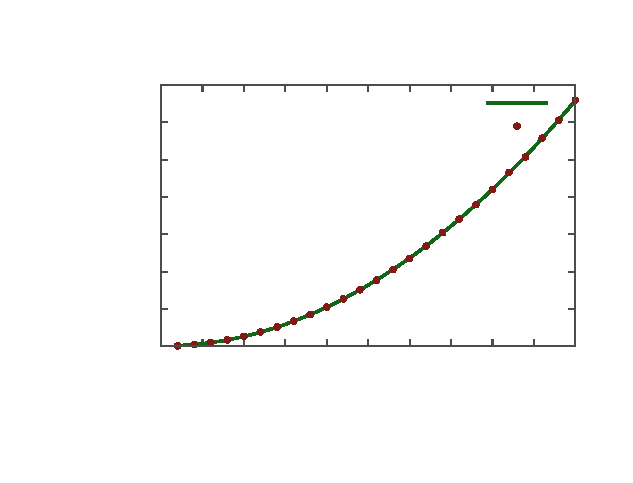
\includegraphics{./graficos/ajuste-seleccion}}%
    \gplfronttext
  \end{picture}%
\endgroup

\end{center}

\subsection*{Eficiencia $\boldsymbol{n log n}$}

La función utilizada para ajustar los valores en estos algoritmos de ordenación es: $f(x) = a_0x + a_1xlog(x)$


\begin{adjustbox}{center}
	\fontsize{6.8pt}{7.2}\selectfont
	\resizebox*{12cm}{!}{
				% GNUPLOT: LaTeX picture with Postscript
\begingroup
  \makeatletter
  \providecommand\color[2][]{%
    \GenericError{(gnuplot) \space\space\space\@spaces}{%
      Package color not loaded in conjunction with
      terminal option `colourtext'%
    }{See the gnuplot documentation for explanation.%
    }{Either use 'blacktext' in gnuplot or load the package
      color.sty in LaTeX.}%
    \renewcommand\color[2][]{}%
  }%
  \providecommand\includegraphics[2][]{%
    \GenericError{(gnuplot) \space\space\space\@spaces}{%
      Package graphicx or graphics not loaded%
    }{See the gnuplot documentation for explanation.%
    }{The gnuplot epslatex terminal needs graphicx.sty or graphics.sty.}%
    \renewcommand\includegraphics[2][]{}%
  }%
  \providecommand\rotatebox[2]{#2}%
  \@ifundefined{ifGPcolor}{%
    \newif\ifGPcolor
    \GPcolortrue
  }{}%
  \@ifundefined{ifGPblacktext}{%
    \newif\ifGPblacktext
    \GPblacktextfalse
  }{}%
  % define a \g@addto@macro without @ in the name:
  \let\gplgaddtomacro\g@addto@macro
  % define empty templates for all commands taking text:
  \gdef\gplbacktext{}%
  \gdef\gplfronttext{}%
  \makeatother
  \ifGPblacktext
    % no textcolor at all
    \def\colorrgb#1{}%
    \def\colorgray#1{}%
  \else
    % gray or color?
    \ifGPcolor
      \def\colorrgb#1{\color[rgb]{#1}}%
      \def\colorgray#1{\color[gray]{#1}}%
      \expandafter\def\csname LTw\endcsname{\color{white}}%
      \expandafter\def\csname LTb\endcsname{\color{black}}%
      \expandafter\def\csname LTa\endcsname{\color{black}}%
      \expandafter\def\csname LT0\endcsname{\color[rgb]{1,0,0}}%
      \expandafter\def\csname LT1\endcsname{\color[rgb]{0,1,0}}%
      \expandafter\def\csname LT2\endcsname{\color[rgb]{0,0,1}}%
      \expandafter\def\csname LT3\endcsname{\color[rgb]{1,0,1}}%
      \expandafter\def\csname LT4\endcsname{\color[rgb]{0,1,1}}%
      \expandafter\def\csname LT5\endcsname{\color[rgb]{1,1,0}}%
      \expandafter\def\csname LT6\endcsname{\color[rgb]{0,0,0}}%
      \expandafter\def\csname LT7\endcsname{\color[rgb]{1,0.3,0}}%
      \expandafter\def\csname LT8\endcsname{\color[rgb]{0.5,0.5,0.5}}%
    \else
      % gray
      \def\colorrgb#1{\color{black}}%
      \def\colorgray#1{\color[gray]{#1}}%
      \expandafter\def\csname LTw\endcsname{\color{white}}%
      \expandafter\def\csname LTb\endcsname{\color{black}}%
      \expandafter\def\csname LTa\endcsname{\color{black}}%
      \expandafter\def\csname LT0\endcsname{\color{black}}%
      \expandafter\def\csname LT1\endcsname{\color{black}}%
      \expandafter\def\csname LT2\endcsname{\color{black}}%
      \expandafter\def\csname LT3\endcsname{\color{black}}%
      \expandafter\def\csname LT4\endcsname{\color{black}}%
      \expandafter\def\csname LT5\endcsname{\color{black}}%
      \expandafter\def\csname LT6\endcsname{\color{black}}%
      \expandafter\def\csname LT7\endcsname{\color{black}}%
      \expandafter\def\csname LT8\endcsname{\color{black}}%
    \fi
  \fi
    \setlength{\unitlength}{0.0500bp}%
    \ifx\gptboxheight\undefined%
      \newlength{\gptboxheight}%
      \newlength{\gptboxwidth}%
      \newsavebox{\gptboxtext}%
    \fi%
    \setlength{\fboxrule}{0.5pt}%
    \setlength{\fboxsep}{1pt}%
\begin{picture}(5760.00,4320.00)%
    \gplgaddtomacro\gplbacktext{%
      \colorrgb{0.30,0.30,0.30}%
      \put(1650,1246){\makebox(0,0)[r]{\strut{}$\textcolor{text}{0.0001}$}}%
      \colorrgb{0.30,0.30,0.30}%
      \put(1650,2050){\makebox(0,0)[r]{\strut{}$\textcolor{text}{0.001}$}}%
      \colorrgb{0.30,0.30,0.30}%
      \put(1650,2855){\makebox(0,0)[r]{\strut{}$\textcolor{text}{0.01}$}}%
      \colorrgb{0.30,0.30,0.30}%
      \put(1650,3659){\makebox(0,0)[r]{\strut{}$\textcolor{text}{0.1}$}}%
      \colorrgb{0.30,0.30,0.30}%
      \put(1782,1114){\rotatebox{45}{\makebox(0,0)[r]{\strut{}$\textcolor{text}{0}$}}}%
      \colorrgb{0.30,0.30,0.30}%
      \put(2230,1114){\rotatebox{45}{\makebox(0,0)[r]{\strut{}$\textcolor{text}{20000}$}}}%
      \colorrgb{0.30,0.30,0.30}%
      \put(2677,1114){\rotatebox{45}{\makebox(0,0)[r]{\strut{}$\textcolor{text}{40000}$}}}%
      \colorrgb{0.30,0.30,0.30}%
      \put(3125,1114){\rotatebox{45}{\makebox(0,0)[r]{\strut{}$\textcolor{text}{60000}$}}}%
      \colorrgb{0.30,0.30,0.30}%
      \put(3573,1114){\rotatebox{45}{\makebox(0,0)[r]{\strut{}$\textcolor{text}{80000}$}}}%
      \colorrgb{0.30,0.30,0.30}%
      \put(4020,1114){\rotatebox{45}{\makebox(0,0)[r]{\strut{}$\textcolor{text}{100000}$}}}%
      \colorrgb{0.30,0.30,0.30}%
      \put(4468,1114){\rotatebox{45}{\makebox(0,0)[r]{\strut{}$\textcolor{text}{120000}$}}}%
      \colorrgb{0.30,0.30,0.30}%
      \put(4915,1114){\rotatebox{45}{\makebox(0,0)[r]{\strut{}$\textcolor{text}{140000}$}}}%
      \colorrgb{0.30,0.30,0.30}%
      \put(5363,1114){\rotatebox{45}{\makebox(0,0)[r]{\strut{}$\textcolor{text}{160000}$}}}%
    }%
    \gplgaddtomacro\gplfronttext{%
      \colorrgb{0.30,0.30,0.30}%
      \put(220,2452){\rotatebox{-270}{\makebox(0,0){\strut{}Tiempo de ejecución (s)}}}%
      \colorrgb{0.30,0.30,0.30}%
      \put(3572,220){\makebox(0,0){\strut{}Tamaño del vector (elementos)}}%
      \colorrgb{0.30,0.30,0.30}%
      \put(3572,3989){\makebox(0,0){\strut{}Ajuste Mergesort}}%
      \csname LTb\endcsname%
      \put(4376,3486){\makebox(0,0)[r]{\strut{}Mergesort ajustado}}%
      \csname LTb\endcsname%
      \put(4376,3266){\makebox(0,0)[r]{\strut{}Mergesort}}%
    }%
    \gplbacktext
    \put(0,0){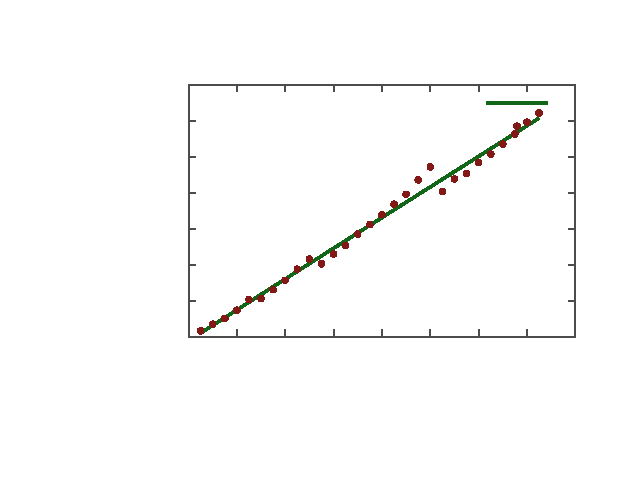
\includegraphics{./graficos/ajuste-mergesort}}%
    \gplfronttext
  \end{picture}%
\endgroup

			}
\end{adjustbox}



\begin{adjustbox}{center}
	\fontsize{6.8pt}{7.2}\selectfont
	\resizebox*{12cm}{!}{
				% GNUPLOT: LaTeX picture with Postscript
\begingroup
  \makeatletter
  \providecommand\color[2][]{%
    \GenericError{(gnuplot) \space\space\space\@spaces}{%
      Package color not loaded in conjunction with
      terminal option `colourtext'%
    }{See the gnuplot documentation for explanation.%
    }{Either use 'blacktext' in gnuplot or load the package
      color.sty in LaTeX.}%
    \renewcommand\color[2][]{}%
  }%
  \providecommand\includegraphics[2][]{%
    \GenericError{(gnuplot) \space\space\space\@spaces}{%
      Package graphicx or graphics not loaded%
    }{See the gnuplot documentation for explanation.%
    }{The gnuplot epslatex terminal needs graphicx.sty or graphics.sty.}%
    \renewcommand\includegraphics[2][]{}%
  }%
  \providecommand\rotatebox[2]{#2}%
  \@ifundefined{ifGPcolor}{%
    \newif\ifGPcolor
    \GPcolortrue
  }{}%
  \@ifundefined{ifGPblacktext}{%
    \newif\ifGPblacktext
    \GPblacktextfalse
  }{}%
  % define a \g@addto@macro without @ in the name:
  \let\gplgaddtomacro\g@addto@macro
  % define empty templates for all commands taking text:
  \gdef\gplbacktext{}%
  \gdef\gplfronttext{}%
  \makeatother
  \ifGPblacktext
    % no textcolor at all
    \def\colorrgb#1{}%
    \def\colorgray#1{}%
  \else
    % gray or color?
    \ifGPcolor
      \def\colorrgb#1{\color[rgb]{#1}}%
      \def\colorgray#1{\color[gray]{#1}}%
      \expandafter\def\csname LTw\endcsname{\color{white}}%
      \expandafter\def\csname LTb\endcsname{\color{black}}%
      \expandafter\def\csname LTa\endcsname{\color{black}}%
      \expandafter\def\csname LT0\endcsname{\color[rgb]{1,0,0}}%
      \expandafter\def\csname LT1\endcsname{\color[rgb]{0,1,0}}%
      \expandafter\def\csname LT2\endcsname{\color[rgb]{0,0,1}}%
      \expandafter\def\csname LT3\endcsname{\color[rgb]{1,0,1}}%
      \expandafter\def\csname LT4\endcsname{\color[rgb]{0,1,1}}%
      \expandafter\def\csname LT5\endcsname{\color[rgb]{1,1,0}}%
      \expandafter\def\csname LT6\endcsname{\color[rgb]{0,0,0}}%
      \expandafter\def\csname LT7\endcsname{\color[rgb]{1,0.3,0}}%
      \expandafter\def\csname LT8\endcsname{\color[rgb]{0.5,0.5,0.5}}%
    \else
      % gray
      \def\colorrgb#1{\color{black}}%
      \def\colorgray#1{\color[gray]{#1}}%
      \expandafter\def\csname LTw\endcsname{\color{white}}%
      \expandafter\def\csname LTb\endcsname{\color{black}}%
      \expandafter\def\csname LTa\endcsname{\color{black}}%
      \expandafter\def\csname LT0\endcsname{\color{black}}%
      \expandafter\def\csname LT1\endcsname{\color{black}}%
      \expandafter\def\csname LT2\endcsname{\color{black}}%
      \expandafter\def\csname LT3\endcsname{\color{black}}%
      \expandafter\def\csname LT4\endcsname{\color{black}}%
      \expandafter\def\csname LT5\endcsname{\color{black}}%
      \expandafter\def\csname LT6\endcsname{\color{black}}%
      \expandafter\def\csname LT7\endcsname{\color{black}}%
      \expandafter\def\csname LT8\endcsname{\color{black}}%
    \fi
  \fi
    \setlength{\unitlength}{0.0500bp}%
    \ifx\gptboxheight\undefined%
      \newlength{\gptboxheight}%
      \newlength{\gptboxwidth}%
      \newsavebox{\gptboxtext}%
    \fi%
    \setlength{\fboxrule}{0.5pt}%
    \setlength{\fboxsep}{1pt}%
\begin{picture}(5760.00,4320.00)%
    \gplgaddtomacro\gplbacktext{%
      \colorrgb{0.30,0.30,0.30}%
      \put(1518,1246){\makebox(0,0)[r]{\strut{}$\textcolor{text}{0}$}}%
      \colorrgb{0.30,0.30,0.30}%
      \put(1518,1591){\makebox(0,0)[r]{\strut{}$\textcolor{text}{0.005}$}}%
      \colorrgb{0.30,0.30,0.30}%
      \put(1518,1935){\makebox(0,0)[r]{\strut{}$\textcolor{text}{0.01}$}}%
      \colorrgb{0.30,0.30,0.30}%
      \put(1518,2280){\makebox(0,0)[r]{\strut{}$\textcolor{text}{0.015}$}}%
      \colorrgb{0.30,0.30,0.30}%
      \put(1518,2625){\makebox(0,0)[r]{\strut{}$\textcolor{text}{0.02}$}}%
      \colorrgb{0.30,0.30,0.30}%
      \put(1518,2970){\makebox(0,0)[r]{\strut{}$\textcolor{text}{0.025}$}}%
      \colorrgb{0.30,0.30,0.30}%
      \put(1518,3314){\makebox(0,0)[r]{\strut{}$\textcolor{text}{0.03}$}}%
      \colorrgb{0.30,0.30,0.30}%
      \put(1518,3659){\makebox(0,0)[r]{\strut{}$\textcolor{text}{0.035}$}}%
      \colorrgb{0.30,0.30,0.30}%
      \put(1650,1114){\rotatebox{45}{\makebox(0,0)[r]{\strut{}$\textcolor{text}{0}$}}}%
      \colorrgb{0.30,0.30,0.30}%
      \put(2114,1114){\rotatebox{45}{\makebox(0,0)[r]{\strut{}$\textcolor{text}{20000}$}}}%
      \colorrgb{0.30,0.30,0.30}%
      \put(2578,1114){\rotatebox{45}{\makebox(0,0)[r]{\strut{}$\textcolor{text}{40000}$}}}%
      \colorrgb{0.30,0.30,0.30}%
      \put(3042,1114){\rotatebox{45}{\makebox(0,0)[r]{\strut{}$\textcolor{text}{60000}$}}}%
      \colorrgb{0.30,0.30,0.30}%
      \put(3507,1114){\rotatebox{45}{\makebox(0,0)[r]{\strut{}$\textcolor{text}{80000}$}}}%
      \colorrgb{0.30,0.30,0.30}%
      \put(3971,1114){\rotatebox{45}{\makebox(0,0)[r]{\strut{}$\textcolor{text}{100000}$}}}%
      \colorrgb{0.30,0.30,0.30}%
      \put(4435,1114){\rotatebox{45}{\makebox(0,0)[r]{\strut{}$\textcolor{text}{120000}$}}}%
      \colorrgb{0.30,0.30,0.30}%
      \put(4899,1114){\rotatebox{45}{\makebox(0,0)[r]{\strut{}$\textcolor{text}{140000}$}}}%
      \colorrgb{0.30,0.30,0.30}%
      \put(5363,1114){\rotatebox{45}{\makebox(0,0)[r]{\strut{}$\textcolor{text}{160000}$}}}%
    }%
    \gplgaddtomacro\gplfronttext{%
      \colorrgb{0.30,0.30,0.30}%
      \put(220,2452){\rotatebox{-270}{\makebox(0,0){\strut{}Tiempo de ejecución (s)}}}%
      \colorrgb{0.30,0.30,0.30}%
      \put(3506,220){\makebox(0,0){\strut{}Tamaño del vector (elementos)}}%
      \colorrgb{0.30,0.30,0.30}%
      \put(3506,3989){\makebox(0,0){\strut{}Ajuste Heapsort}}%
      \csname LTb\endcsname%
      \put(4376,3486){\makebox(0,0)[r]{\strut{}1.20e-11$ \cdot x^{7.04e-01}+x \cdot 1.60e-07$}}%
      \csname LTb\endcsname%
      \put(4376,3266){\makebox(0,0)[r]{\strut{}Heapsort}}%
    }%
    \gplbacktext
    \put(0,0){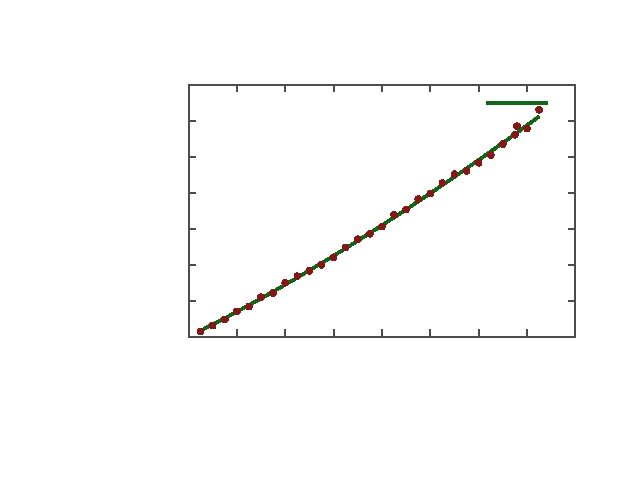
\includegraphics{./graficos/ajuste-heapsort}}%
    \gplfronttext
  \end{picture}%
\endgroup

			}
\end{adjustbox}

\begin{adjustbox}{center}
	\fontsize{6.8pt}{7.2}\selectfont
	\resizebox*{12cm}{!}{
				% GNUPLOT: LaTeX picture with Postscript
\begingroup
  \makeatletter
  \providecommand\color[2][]{%
    \GenericError{(gnuplot) \space\space\space\@spaces}{%
      Package color not loaded in conjunction with
      terminal option `colourtext'%
    }{See the gnuplot documentation for explanation.%
    }{Either use 'blacktext' in gnuplot or load the package
      color.sty in LaTeX.}%
    \renewcommand\color[2][]{}%
  }%
  \providecommand\includegraphics[2][]{%
    \GenericError{(gnuplot) \space\space\space\@spaces}{%
      Package graphicx or graphics not loaded%
    }{See the gnuplot documentation for explanation.%
    }{The gnuplot epslatex terminal needs graphicx.sty or graphics.sty.}%
    \renewcommand\includegraphics[2][]{}%
  }%
  \providecommand\rotatebox[2]{#2}%
  \@ifundefined{ifGPcolor}{%
    \newif\ifGPcolor
    \GPcolortrue
  }{}%
  \@ifundefined{ifGPblacktext}{%
    \newif\ifGPblacktext
    \GPblacktextfalse
  }{}%
  % define a \g@addto@macro without @ in the name:
  \let\gplgaddtomacro\g@addto@macro
  % define empty templates for all commands taking text:
  \gdef\gplbacktext{}%
  \gdef\gplfronttext{}%
  \makeatother
  \ifGPblacktext
    % no textcolor at all
    \def\colorrgb#1{}%
    \def\colorgray#1{}%
  \else
    % gray or color?
    \ifGPcolor
      \def\colorrgb#1{\color[rgb]{#1}}%
      \def\colorgray#1{\color[gray]{#1}}%
      \expandafter\def\csname LTw\endcsname{\color{white}}%
      \expandafter\def\csname LTb\endcsname{\color{black}}%
      \expandafter\def\csname LTa\endcsname{\color{black}}%
      \expandafter\def\csname LT0\endcsname{\color[rgb]{1,0,0}}%
      \expandafter\def\csname LT1\endcsname{\color[rgb]{0,1,0}}%
      \expandafter\def\csname LT2\endcsname{\color[rgb]{0,0,1}}%
      \expandafter\def\csname LT3\endcsname{\color[rgb]{1,0,1}}%
      \expandafter\def\csname LT4\endcsname{\color[rgb]{0,1,1}}%
      \expandafter\def\csname LT5\endcsname{\color[rgb]{1,1,0}}%
      \expandafter\def\csname LT6\endcsname{\color[rgb]{0,0,0}}%
      \expandafter\def\csname LT7\endcsname{\color[rgb]{1,0.3,0}}%
      \expandafter\def\csname LT8\endcsname{\color[rgb]{0.5,0.5,0.5}}%
    \else
      % gray
      \def\colorrgb#1{\color{black}}%
      \def\colorgray#1{\color[gray]{#1}}%
      \expandafter\def\csname LTw\endcsname{\color{white}}%
      \expandafter\def\csname LTb\endcsname{\color{black}}%
      \expandafter\def\csname LTa\endcsname{\color{black}}%
      \expandafter\def\csname LT0\endcsname{\color{black}}%
      \expandafter\def\csname LT1\endcsname{\color{black}}%
      \expandafter\def\csname LT2\endcsname{\color{black}}%
      \expandafter\def\csname LT3\endcsname{\color{black}}%
      \expandafter\def\csname LT4\endcsname{\color{black}}%
      \expandafter\def\csname LT5\endcsname{\color{black}}%
      \expandafter\def\csname LT6\endcsname{\color{black}}%
      \expandafter\def\csname LT7\endcsname{\color{black}}%
      \expandafter\def\csname LT8\endcsname{\color{black}}%
    \fi
  \fi
    \setlength{\unitlength}{0.0500bp}%
    \ifx\gptboxheight\undefined%
      \newlength{\gptboxheight}%
      \newlength{\gptboxwidth}%
      \newsavebox{\gptboxtext}%
    \fi%
    \setlength{\fboxrule}{0.5pt}%
    \setlength{\fboxsep}{1pt}%
\begin{picture}(5760.00,4320.00)%
    \gplgaddtomacro\gplbacktext{%
      \colorrgb{0.30,0.30,0.30}%
      \put(1518,1246){\makebox(0,0)[r]{\strut{}$\textcolor{text}{0}$}}%
      \colorrgb{0.30,0.30,0.30}%
      \put(1518,1729){\makebox(0,0)[r]{\strut{}$\textcolor{text}{0.005}$}}%
      \colorrgb{0.30,0.30,0.30}%
      \put(1518,2211){\makebox(0,0)[r]{\strut{}$\textcolor{text}{0.01}$}}%
      \colorrgb{0.30,0.30,0.30}%
      \put(1518,2694){\makebox(0,0)[r]{\strut{}$\textcolor{text}{0.015}$}}%
      \colorrgb{0.30,0.30,0.30}%
      \put(1518,3176){\makebox(0,0)[r]{\strut{}$\textcolor{text}{0.02}$}}%
      \colorrgb{0.30,0.30,0.30}%
      \put(1518,3659){\makebox(0,0)[r]{\strut{}$\textcolor{text}{0.025}$}}%
      \colorrgb{0.30,0.30,0.30}%
      \put(1650,1114){\rotatebox{45}{\makebox(0,0)[r]{\strut{}$\textcolor{text}{0}$}}}%
      \colorrgb{0.30,0.30,0.30}%
      \put(2114,1114){\rotatebox{45}{\makebox(0,0)[r]{\strut{}$\textcolor{text}{20000}$}}}%
      \colorrgb{0.30,0.30,0.30}%
      \put(2578,1114){\rotatebox{45}{\makebox(0,0)[r]{\strut{}$\textcolor{text}{40000}$}}}%
      \colorrgb{0.30,0.30,0.30}%
      \put(3042,1114){\rotatebox{45}{\makebox(0,0)[r]{\strut{}$\textcolor{text}{60000}$}}}%
      \colorrgb{0.30,0.30,0.30}%
      \put(3507,1114){\rotatebox{45}{\makebox(0,0)[r]{\strut{}$\textcolor{text}{80000}$}}}%
      \colorrgb{0.30,0.30,0.30}%
      \put(3971,1114){\rotatebox{45}{\makebox(0,0)[r]{\strut{}$\textcolor{text}{100000}$}}}%
      \colorrgb{0.30,0.30,0.30}%
      \put(4435,1114){\rotatebox{45}{\makebox(0,0)[r]{\strut{}$\textcolor{text}{120000}$}}}%
      \colorrgb{0.30,0.30,0.30}%
      \put(4899,1114){\rotatebox{45}{\makebox(0,0)[r]{\strut{}$\textcolor{text}{140000}$}}}%
      \colorrgb{0.30,0.30,0.30}%
      \put(5363,1114){\rotatebox{45}{\makebox(0,0)[r]{\strut{}$\textcolor{text}{160000}$}}}%
    }%
    \gplgaddtomacro\gplfronttext{%
      \colorrgb{0.30,0.30,0.30}%
      \put(220,2452){\rotatebox{-270}{\makebox(0,0){\strut{}Tiempo de ejecución (s)}}}%
      \colorrgb{0.30,0.30,0.30}%
      \put(3506,220){\makebox(0,0){\strut{}Tamaño del vector (elementos)}}%
      \colorrgb{0.30,0.30,0.30}%
      \put(3506,3989){\makebox(0,0){\strut{}Ajuste Quicksort}}%
      \csname LTb\endcsname%
      \put(4376,3486){\makebox(0,0)[r]{\strut{}$ 1.14e-08 \cdot x\log x + 7.66e-09 x + 4.91e-06$}}%
      \csname LTb\endcsname%
      \put(4376,3266){\makebox(0,0)[r]{\strut{}Quicksort}}%
    }%
    \gplbacktext
    \put(0,0){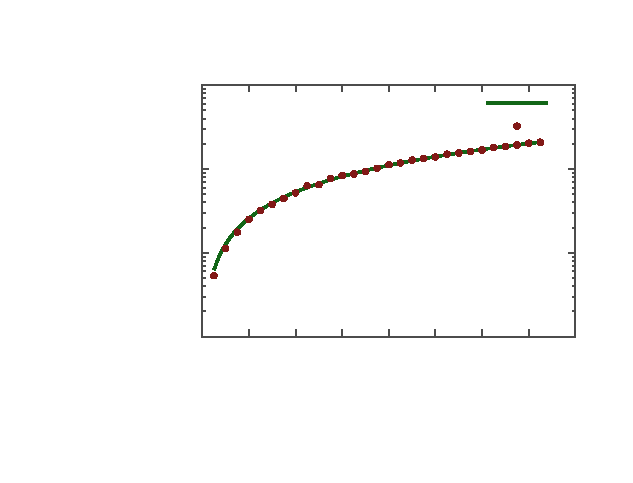
\includegraphics{./graficos/ajuste-quicksort}}%
    \gplfronttext
  \end{picture}%
\endgroup

			}
\end{adjustbox}

\subsection*{Eficiencia $\boldsymbol{n^3}$}

En el caso del algoritmo de Floyd la función $f(x)$ utilizada es: $f(x) = a_0x^3 + a_1x^2 + a_2x + a_3$.

\begin{adjustbox}{center}
	\fontsize{8pt}{7.2}\selectfont
	\resizebox*{13cm}{!}{
				% GNUPLOT: LaTeX picture with Postscript
\begingroup
  \makeatletter
  \providecommand\color[2][]{%
    \GenericError{(gnuplot) \space\space\space\@spaces}{%
      Package color not loaded in conjunction with
      terminal option `colourtext'%
    }{See the gnuplot documentation for explanation.%
    }{Either use 'blacktext' in gnuplot or load the package
      color.sty in LaTeX.}%
    \renewcommand\color[2][]{}%
  }%
  \providecommand\includegraphics[2][]{%
    \GenericError{(gnuplot) \space\space\space\@spaces}{%
      Package graphicx or graphics not loaded%
    }{See the gnuplot documentation for explanation.%
    }{The gnuplot epslatex terminal needs graphicx.sty or graphics.sty.}%
    \renewcommand\includegraphics[2][]{}%
  }%
  \providecommand\rotatebox[2]{#2}%
  \@ifundefined{ifGPcolor}{%
    \newif\ifGPcolor
    \GPcolortrue
  }{}%
  \@ifundefined{ifGPblacktext}{%
    \newif\ifGPblacktext
    \GPblacktextfalse
  }{}%
  % define a \g@addto@macro without @ in the name:
  \let\gplgaddtomacro\g@addto@macro
  % define empty templates for all commands taking text:
  \gdef\gplbacktext{}%
  \gdef\gplfronttext{}%
  \makeatother
  \ifGPblacktext
    % no textcolor at all
    \def\colorrgb#1{}%
    \def\colorgray#1{}%
  \else
    % gray or color?
    \ifGPcolor
      \def\colorrgb#1{\color[rgb]{#1}}%
      \def\colorgray#1{\color[gray]{#1}}%
      \expandafter\def\csname LTw\endcsname{\color{white}}%
      \expandafter\def\csname LTb\endcsname{\color{black}}%
      \expandafter\def\csname LTa\endcsname{\color{black}}%
      \expandafter\def\csname LT0\endcsname{\color[rgb]{1,0,0}}%
      \expandafter\def\csname LT1\endcsname{\color[rgb]{0,1,0}}%
      \expandafter\def\csname LT2\endcsname{\color[rgb]{0,0,1}}%
      \expandafter\def\csname LT3\endcsname{\color[rgb]{1,0,1}}%
      \expandafter\def\csname LT4\endcsname{\color[rgb]{0,1,1}}%
      \expandafter\def\csname LT5\endcsname{\color[rgb]{1,1,0}}%
      \expandafter\def\csname LT6\endcsname{\color[rgb]{0,0,0}}%
      \expandafter\def\csname LT7\endcsname{\color[rgb]{1,0.3,0}}%
      \expandafter\def\csname LT8\endcsname{\color[rgb]{0.5,0.5,0.5}}%
    \else
      % gray
      \def\colorrgb#1{\color{black}}%
      \def\colorgray#1{\color[gray]{#1}}%
      \expandafter\def\csname LTw\endcsname{\color{white}}%
      \expandafter\def\csname LTb\endcsname{\color{black}}%
      \expandafter\def\csname LTa\endcsname{\color{black}}%
      \expandafter\def\csname LT0\endcsname{\color{black}}%
      \expandafter\def\csname LT1\endcsname{\color{black}}%
      \expandafter\def\csname LT2\endcsname{\color{black}}%
      \expandafter\def\csname LT3\endcsname{\color{black}}%
      \expandafter\def\csname LT4\endcsname{\color{black}}%
      \expandafter\def\csname LT5\endcsname{\color{black}}%
      \expandafter\def\csname LT6\endcsname{\color{black}}%
      \expandafter\def\csname LT7\endcsname{\color{black}}%
      \expandafter\def\csname LT8\endcsname{\color{black}}%
    \fi
  \fi
    \setlength{\unitlength}{0.0500bp}%
    \ifx\gptboxheight\undefined%
      \newlength{\gptboxheight}%
      \newlength{\gptboxwidth}%
      \newsavebox{\gptboxtext}%
    \fi%
    \setlength{\fboxrule}{0.5pt}%
    \setlength{\fboxsep}{1pt}%
\begin{picture}(5760.00,4320.00)%
    \gplgaddtomacro\gplbacktext{%
      \colorrgb{0.30,0.30,0.30}%
      \put(1122,1060){\makebox(0,0)[r]{\strut{}$\textcolor{text}{0}$}}%
      \colorrgb{0.30,0.30,0.30}%
      \put(1122,1349){\makebox(0,0)[r]{\strut{}$\textcolor{text}{2}$}}%
      \colorrgb{0.30,0.30,0.30}%
      \put(1122,1638){\makebox(0,0)[r]{\strut{}$\textcolor{text}{4}$}}%
      \colorrgb{0.30,0.30,0.30}%
      \put(1122,1926){\makebox(0,0)[r]{\strut{}$\textcolor{text}{6}$}}%
      \colorrgb{0.30,0.30,0.30}%
      \put(1122,2215){\makebox(0,0)[r]{\strut{}$\textcolor{text}{8}$}}%
      \colorrgb{0.30,0.30,0.30}%
      \put(1122,2504){\makebox(0,0)[r]{\strut{}$\textcolor{text}{10}$}}%
      \colorrgb{0.30,0.30,0.30}%
      \put(1122,2793){\makebox(0,0)[r]{\strut{}$\textcolor{text}{12}$}}%
      \colorrgb{0.30,0.30,0.30}%
      \put(1122,3081){\makebox(0,0)[r]{\strut{}$\textcolor{text}{14}$}}%
      \colorrgb{0.30,0.30,0.30}%
      \put(1122,3370){\makebox(0,0)[r]{\strut{}$\textcolor{text}{16}$}}%
      \colorrgb{0.30,0.30,0.30}%
      \put(1122,3659){\makebox(0,0)[r]{\strut{}$\textcolor{text}{18}$}}%
      \colorrgb{0.30,0.30,0.30}%
      \put(1254,928){\rotatebox{45}{\makebox(0,0)[r]{\strut{}$\textcolor{text}{0}$}}}%
      \colorrgb{0.30,0.30,0.30}%
      \put(1768,928){\rotatebox{45}{\makebox(0,0)[r]{\strut{}$\textcolor{text}{200}$}}}%
      \colorrgb{0.30,0.30,0.30}%
      \put(2281,928){\rotatebox{45}{\makebox(0,0)[r]{\strut{}$\textcolor{text}{400}$}}}%
      \colorrgb{0.30,0.30,0.30}%
      \put(2795,928){\rotatebox{45}{\makebox(0,0)[r]{\strut{}$\textcolor{text}{600}$}}}%
      \colorrgb{0.30,0.30,0.30}%
      \put(3309,928){\rotatebox{45}{\makebox(0,0)[r]{\strut{}$\textcolor{text}{800}$}}}%
      \colorrgb{0.30,0.30,0.30}%
      \put(3822,928){\rotatebox{45}{\makebox(0,0)[r]{\strut{}$\textcolor{text}{1000}$}}}%
      \colorrgb{0.30,0.30,0.30}%
      \put(4336,928){\rotatebox{45}{\makebox(0,0)[r]{\strut{}$\textcolor{text}{1200}$}}}%
      \colorrgb{0.30,0.30,0.30}%
      \put(4849,928){\rotatebox{45}{\makebox(0,0)[r]{\strut{}$\textcolor{text}{1400}$}}}%
      \colorrgb{0.30,0.30,0.30}%
      \put(5363,928){\rotatebox{45}{\makebox(0,0)[r]{\strut{}$\textcolor{text}{1600}$}}}%
    }%
    \gplgaddtomacro\gplfronttext{%
      \colorrgb{0.30,0.30,0.30}%
      \put(220,2359){\rotatebox{-270}{\makebox(0,0){\strut{}Tiempo de ejecución (s)}}}%
      \colorrgb{0.30,0.30,0.30}%
      \put(3308,220){\makebox(0,0){\strut{}Tamaño del vector (elementos)}}%
      \colorrgb{0.30,0.30,0.30}%
      \put(3308,3989){\makebox(0,0){\strut{}Ajuste Floyd}}%
      \csname LTb\endcsname%
      \put(4376,3486){\makebox(0,0)[r]{\strut{}5.38e-09$x^3$+4.48e-07$x^2$+-2.70e-04$x$+3.11e-02}}%
      \csname LTb\endcsname%
      \put(4376,3266){\makebox(0,0)[r]{\strut{}Floyd}}%
    }%
    \gplbacktext
    \put(0,0){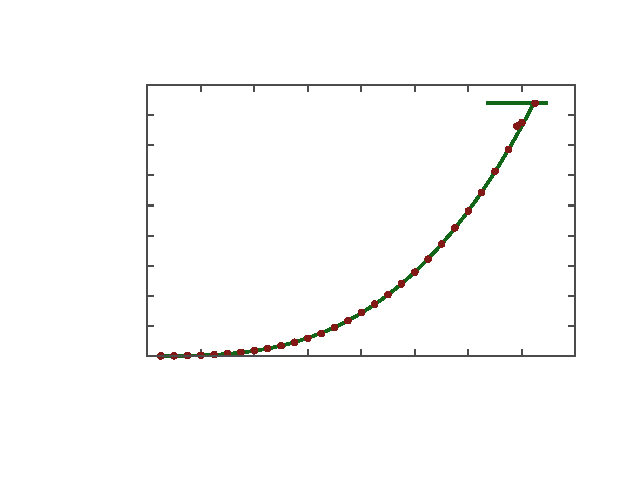
\includegraphics{./graficos/ajuste-floyd}}%
    \gplfronttext
  \end{picture}%
\endgroup

			}
\end{adjustbox}

\subsection*{Eficiencia $\boldsymbol{2^n}$}

Por último, ajustamos el algoritmo de Hanoi mediante la función: $f(x) = a_02^{a_{1}x + a_2}$ obteniendo el resultado mostrado a continuación.
 
\begin{center}
	% GNUPLOT: LaTeX picture with Postscript
\begingroup
  \makeatletter
  \providecommand\color[2][]{%
    \GenericError{(gnuplot) \space\space\space\@spaces}{%
      Package color not loaded in conjunction with
      terminal option `colourtext'%
    }{See the gnuplot documentation for explanation.%
    }{Either use 'blacktext' in gnuplot or load the package
      color.sty in LaTeX.}%
    \renewcommand\color[2][]{}%
  }%
  \providecommand\includegraphics[2][]{%
    \GenericError{(gnuplot) \space\space\space\@spaces}{%
      Package graphicx or graphics not loaded%
    }{See the gnuplot documentation for explanation.%
    }{The gnuplot epslatex terminal needs graphicx.sty or graphics.sty.}%
    \renewcommand\includegraphics[2][]{}%
  }%
  \providecommand\rotatebox[2]{#2}%
  \@ifundefined{ifGPcolor}{%
    \newif\ifGPcolor
    \GPcolortrue
  }{}%
  \@ifundefined{ifGPblacktext}{%
    \newif\ifGPblacktext
    \GPblacktextfalse
  }{}%
  % define a \g@addto@macro without @ in the name:
  \let\gplgaddtomacro\g@addto@macro
  % define empty templates for all commands taking text:
  \gdef\gplbacktext{}%
  \gdef\gplfronttext{}%
  \makeatother
  \ifGPblacktext
    % no textcolor at all
    \def\colorrgb#1{}%
    \def\colorgray#1{}%
  \else
    % gray or color?
    \ifGPcolor
      \def\colorrgb#1{\color[rgb]{#1}}%
      \def\colorgray#1{\color[gray]{#1}}%
      \expandafter\def\csname LTw\endcsname{\color{white}}%
      \expandafter\def\csname LTb\endcsname{\color{black}}%
      \expandafter\def\csname LTa\endcsname{\color{black}}%
      \expandafter\def\csname LT0\endcsname{\color[rgb]{1,0,0}}%
      \expandafter\def\csname LT1\endcsname{\color[rgb]{0,1,0}}%
      \expandafter\def\csname LT2\endcsname{\color[rgb]{0,0,1}}%
      \expandafter\def\csname LT3\endcsname{\color[rgb]{1,0,1}}%
      \expandafter\def\csname LT4\endcsname{\color[rgb]{0,1,1}}%
      \expandafter\def\csname LT5\endcsname{\color[rgb]{1,1,0}}%
      \expandafter\def\csname LT6\endcsname{\color[rgb]{0,0,0}}%
      \expandafter\def\csname LT7\endcsname{\color[rgb]{1,0.3,0}}%
      \expandafter\def\csname LT8\endcsname{\color[rgb]{0.5,0.5,0.5}}%
    \else
      % gray
      \def\colorrgb#1{\color{black}}%
      \def\colorgray#1{\color[gray]{#1}}%
      \expandafter\def\csname LTw\endcsname{\color{white}}%
      \expandafter\def\csname LTb\endcsname{\color{black}}%
      \expandafter\def\csname LTa\endcsname{\color{black}}%
      \expandafter\def\csname LT0\endcsname{\color{black}}%
      \expandafter\def\csname LT1\endcsname{\color{black}}%
      \expandafter\def\csname LT2\endcsname{\color{black}}%
      \expandafter\def\csname LT3\endcsname{\color{black}}%
      \expandafter\def\csname LT4\endcsname{\color{black}}%
      \expandafter\def\csname LT5\endcsname{\color{black}}%
      \expandafter\def\csname LT6\endcsname{\color{black}}%
      \expandafter\def\csname LT7\endcsname{\color{black}}%
      \expandafter\def\csname LT8\endcsname{\color{black}}%
    \fi
  \fi
    \setlength{\unitlength}{0.0500bp}%
    \ifx\gptboxheight\undefined%
      \newlength{\gptboxheight}%
      \newlength{\gptboxwidth}%
      \newsavebox{\gptboxtext}%
    \fi%
    \setlength{\fboxrule}{0.5pt}%
    \setlength{\fboxsep}{1pt}%
\begin{picture}(5760.00,4320.00)%
    \gplgaddtomacro\gplbacktext{%
      \colorrgb{0.30,0.30,0.30}%
      \put(990,873){\makebox(0,0)[r]{\strut{}$\textcolor{text}{0}$}}%
      \colorrgb{0.30,0.30,0.30}%
      \put(990,1271){\makebox(0,0)[r]{\strut{}$\textcolor{text}{1}$}}%
      \colorrgb{0.30,0.30,0.30}%
      \put(990,1669){\makebox(0,0)[r]{\strut{}$\textcolor{text}{2}$}}%
      \colorrgb{0.30,0.30,0.30}%
      \put(990,2067){\makebox(0,0)[r]{\strut{}$\textcolor{text}{3}$}}%
      \colorrgb{0.30,0.30,0.30}%
      \put(990,2465){\makebox(0,0)[r]{\strut{}$\textcolor{text}{4}$}}%
      \colorrgb{0.30,0.30,0.30}%
      \put(990,2863){\makebox(0,0)[r]{\strut{}$\textcolor{text}{5}$}}%
      \colorrgb{0.30,0.30,0.30}%
      \put(990,3261){\makebox(0,0)[r]{\strut{}$\textcolor{text}{6}$}}%
      \colorrgb{0.30,0.30,0.30}%
      \put(990,3659){\makebox(0,0)[r]{\strut{}$\textcolor{text}{7}$}}%
      \colorrgb{0.30,0.30,0.30}%
      \put(1122,741){\rotatebox{45}{\makebox(0,0)[r]{\strut{}$\textcolor{text}{5}$}}}%
      \colorrgb{0.30,0.30,0.30}%
      \put(1970,741){\rotatebox{45}{\makebox(0,0)[r]{\strut{}$\textcolor{text}{10}$}}}%
      \colorrgb{0.30,0.30,0.30}%
      \put(2818,741){\rotatebox{45}{\makebox(0,0)[r]{\strut{}$\textcolor{text}{15}$}}}%
      \colorrgb{0.30,0.30,0.30}%
      \put(3667,741){\rotatebox{45}{\makebox(0,0)[r]{\strut{}$\textcolor{text}{20}$}}}%
      \colorrgb{0.30,0.30,0.30}%
      \put(4515,741){\rotatebox{45}{\makebox(0,0)[r]{\strut{}$\textcolor{text}{25}$}}}%
      \colorrgb{0.30,0.30,0.30}%
      \put(5363,741){\rotatebox{45}{\makebox(0,0)[r]{\strut{}$\textcolor{text}{30}$}}}%
    }%
    \gplgaddtomacro\gplfronttext{%
      \colorrgb{0.30,0.30,0.30}%
      \put(220,2266){\rotatebox{-270}{\makebox(0,0){\strut{}Tiempo de ejecución (s)}}}%
      \colorrgb{0.30,0.30,0.30}%
      \put(3242,220){\makebox(0,0){\strut{}Tamaño del vector (elementos)}}%
      \colorrgb{0.30,0.30,0.30}%
      \put(3242,3989){\makebox(0,0){\strut{}Ajuste hanoi}}%
      \csname LTb\endcsname%
      \put(4376,3486){\makebox(0,0)[r]{\strut{}Hanoi ajustado}}%
      \csname LTb\endcsname%
      \put(4376,3266){\makebox(0,0)[r]{\strut{}Hanoi}}%
    }%
    \gplbacktext
    \put(0,0){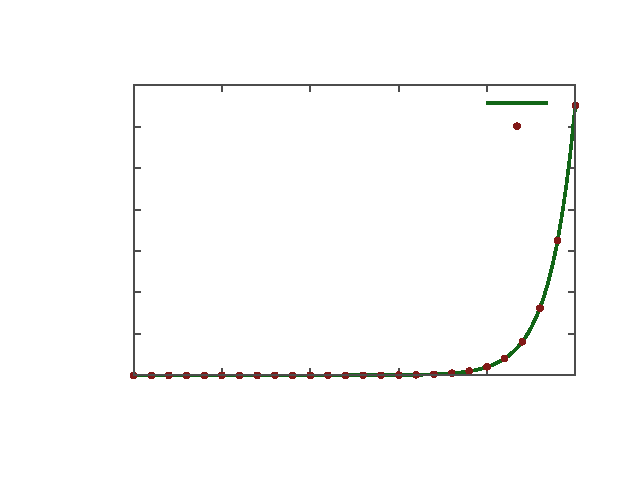
\includegraphics{./graficos/ajuste-hanoi}}%
    \gplfronttext
  \end{picture}%
\endgroup

\end{center}


\section*{Comparativa según optimización y sistema operativo}
Hemos elegido un representante de cada orden de eficiencia, y hemos realizados una comprativa para analizar cómo varían los tiempos de ejecución según el sistema operativo y el nivel de optimización.\\

Para cada algoritmo veremos dos gráficas: una que compara la ejecución sin optimización en los sistemas operativos macOS y Linux; y otra que compara la ejecución en Linux con los distintos tipos de ejecución.

%%Grafica optimización
\subsection*{Representante de $\boldsymbol{O(n^2)}$}
	\begin{center}
		% GNUPLOT: LaTeX picture with Postscript
\begingroup
  \makeatletter
  \providecommand\color[2][]{%
    \GenericError{(gnuplot) \space\space\space\@spaces}{%
      Package color not loaded in conjunction with
      terminal option `colourtext'%
    }{See the gnuplot documentation for explanation.%
    }{Either use 'blacktext' in gnuplot or load the package
      color.sty in LaTeX.}%
    \renewcommand\color[2][]{}%
  }%
  \providecommand\includegraphics[2][]{%
    \GenericError{(gnuplot) \space\space\space\@spaces}{%
      Package graphicx or graphics not loaded%
    }{See the gnuplot documentation for explanation.%
    }{The gnuplot epslatex terminal needs graphicx.sty or graphics.sty.}%
    \renewcommand\includegraphics[2][]{}%
  }%
  \providecommand\rotatebox[2]{#2}%
  \@ifundefined{ifGPcolor}{%
    \newif\ifGPcolor
    \GPcolortrue
  }{}%
  \@ifundefined{ifGPblacktext}{%
    \newif\ifGPblacktext
    \GPblacktextfalse
  }{}%
  % define a \g@addto@macro without @ in the name:
  \let\gplgaddtomacro\g@addto@macro
  % define empty templates for all commands taking text:
  \gdef\gplbacktext{}%
  \gdef\gplfronttext{}%
  \makeatother
  \ifGPblacktext
    % no textcolor at all
    \def\colorrgb#1{}%
    \def\colorgray#1{}%
  \else
    % gray or color?
    \ifGPcolor
      \def\colorrgb#1{\color[rgb]{#1}}%
      \def\colorgray#1{\color[gray]{#1}}%
      \expandafter\def\csname LTw\endcsname{\color{white}}%
      \expandafter\def\csname LTb\endcsname{\color{black}}%
      \expandafter\def\csname LTa\endcsname{\color{black}}%
      \expandafter\def\csname LT0\endcsname{\color[rgb]{1,0,0}}%
      \expandafter\def\csname LT1\endcsname{\color[rgb]{0,1,0}}%
      \expandafter\def\csname LT2\endcsname{\color[rgb]{0,0,1}}%
      \expandafter\def\csname LT3\endcsname{\color[rgb]{1,0,1}}%
      \expandafter\def\csname LT4\endcsname{\color[rgb]{0,1,1}}%
      \expandafter\def\csname LT5\endcsname{\color[rgb]{1,1,0}}%
      \expandafter\def\csname LT6\endcsname{\color[rgb]{0,0,0}}%
      \expandafter\def\csname LT7\endcsname{\color[rgb]{1,0.3,0}}%
      \expandafter\def\csname LT8\endcsname{\color[rgb]{0.5,0.5,0.5}}%
    \else
      % gray
      \def\colorrgb#1{\color{black}}%
      \def\colorgray#1{\color[gray]{#1}}%
      \expandafter\def\csname LTw\endcsname{\color{white}}%
      \expandafter\def\csname LTb\endcsname{\color{black}}%
      \expandafter\def\csname LTa\endcsname{\color{black}}%
      \expandafter\def\csname LT0\endcsname{\color{black}}%
      \expandafter\def\csname LT1\endcsname{\color{black}}%
      \expandafter\def\csname LT2\endcsname{\color{black}}%
      \expandafter\def\csname LT3\endcsname{\color{black}}%
      \expandafter\def\csname LT4\endcsname{\color{black}}%
      \expandafter\def\csname LT5\endcsname{\color{black}}%
      \expandafter\def\csname LT6\endcsname{\color{black}}%
      \expandafter\def\csname LT7\endcsname{\color{black}}%
      \expandafter\def\csname LT8\endcsname{\color{black}}%
    \fi
  \fi
    \setlength{\unitlength}{0.0500bp}%
    \ifx\gptboxheight\undefined%
      \newlength{\gptboxheight}%
      \newlength{\gptboxwidth}%
      \newsavebox{\gptboxtext}%
    \fi%
    \setlength{\fboxrule}{0.5pt}%
    \setlength{\fboxsep}{1pt}%
\begin{picture}(5760.00,4320.00)%
    \gplgaddtomacro\gplbacktext{%
      \colorrgb{0.30,0.30,0.30}%
      \put(1254,1153){\makebox(0,0)[r]{\strut{}$\textcolor{text}{0}$}}%
      \colorrgb{0.30,0.30,0.30}%
      \put(1254,1571){\makebox(0,0)[r]{\strut{}$\textcolor{text}{0.5}$}}%
      \colorrgb{0.30,0.30,0.30}%
      \put(1254,1988){\makebox(0,0)[r]{\strut{}$\textcolor{text}{1}$}}%
      \colorrgb{0.30,0.30,0.30}%
      \put(1254,2406){\makebox(0,0)[r]{\strut{}$\textcolor{text}{1.5}$}}%
      \colorrgb{0.30,0.30,0.30}%
      \put(1254,2824){\makebox(0,0)[r]{\strut{}$\textcolor{text}{2}$}}%
      \colorrgb{0.30,0.30,0.30}%
      \put(1254,3241){\makebox(0,0)[r]{\strut{}$\textcolor{text}{2.5}$}}%
      \colorrgb{0.30,0.30,0.30}%
      \put(1254,3659){\makebox(0,0)[r]{\strut{}$\textcolor{text}{3}$}}%
      \colorrgb{0.30,0.30,0.30}%
      \put(1386,1021){\rotatebox{45}{\makebox(0,0)[r]{\strut{}$\textcolor{text}{0}$}}}%
      \colorrgb{0.30,0.30,0.30}%
      \put(1784,1021){\rotatebox{45}{\makebox(0,0)[r]{\strut{}$\textcolor{text}{5000}$}}}%
      \colorrgb{0.30,0.30,0.30}%
      \put(2181,1021){\rotatebox{45}{\makebox(0,0)[r]{\strut{}$\textcolor{text}{10000}$}}}%
      \colorrgb{0.30,0.30,0.30}%
      \put(2579,1021){\rotatebox{45}{\makebox(0,0)[r]{\strut{}$\textcolor{text}{15000}$}}}%
      \colorrgb{0.30,0.30,0.30}%
      \put(2977,1021){\rotatebox{45}{\makebox(0,0)[r]{\strut{}$\textcolor{text}{20000}$}}}%
      \colorrgb{0.30,0.30,0.30}%
      \put(3375,1021){\rotatebox{45}{\makebox(0,0)[r]{\strut{}$\textcolor{text}{25000}$}}}%
      \colorrgb{0.30,0.30,0.30}%
      \put(3772,1021){\rotatebox{45}{\makebox(0,0)[r]{\strut{}$\textcolor{text}{30000}$}}}%
      \colorrgb{0.30,0.30,0.30}%
      \put(4170,1021){\rotatebox{45}{\makebox(0,0)[r]{\strut{}$\textcolor{text}{35000}$}}}%
      \colorrgb{0.30,0.30,0.30}%
      \put(4568,1021){\rotatebox{45}{\makebox(0,0)[r]{\strut{}$\textcolor{text}{40000}$}}}%
      \colorrgb{0.30,0.30,0.30}%
      \put(4965,1021){\rotatebox{45}{\makebox(0,0)[r]{\strut{}$\textcolor{text}{45000}$}}}%
      \colorrgb{0.30,0.30,0.30}%
      \put(5363,1021){\rotatebox{45}{\makebox(0,0)[r]{\strut{}$\textcolor{text}{50000}$}}}%
    }%
    \gplgaddtomacro\gplfronttext{%
      \colorrgb{0.30,0.30,0.30}%
      \put(220,2406){\rotatebox{-270}{\makebox(0,0){\strut{}Tiempo de ejecución (s)}}}%
      \colorrgb{0.30,0.30,0.30}%
      \put(3374,220){\makebox(0,0){\strut{}Tamaño del vector (elementos)}}%
      \colorrgb{0.30,0.30,0.30}%
      \put(3374,3989){\makebox(0,0){\strut{}Comparación inserción en macOS y Linux}}%
      \csname LTb\endcsname%
      \put(4376,3486){\makebox(0,0)[r]{\strut{}Linux}}%
      \csname LTb\endcsname%
      \put(4376,3266){\makebox(0,0)[r]{\strut{}Mac}}%
    }%
    \gplbacktext
    \put(0,0){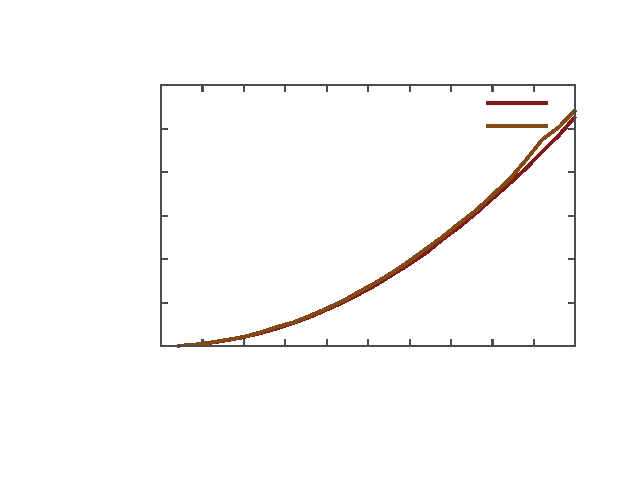
\includegraphics{./graficos/insercion-maclinux}}%
    \gplfronttext
  \end{picture}%
\endgroup

	\end{center}

	\begin{center}
		% GNUPLOT: LaTeX picture with Postscript
\begingroup
  \makeatletter
  \providecommand\color[2][]{%
    \GenericError{(gnuplot) \space\space\space\@spaces}{%
      Package color not loaded in conjunction with
      terminal option `colourtext'%
    }{See the gnuplot documentation for explanation.%
    }{Either use 'blacktext' in gnuplot or load the package
      color.sty in LaTeX.}%
    \renewcommand\color[2][]{}%
  }%
  \providecommand\includegraphics[2][]{%
    \GenericError{(gnuplot) \space\space\space\@spaces}{%
      Package graphicx or graphics not loaded%
    }{See the gnuplot documentation for explanation.%
    }{The gnuplot epslatex terminal needs graphicx.sty or graphics.sty.}%
    \renewcommand\includegraphics[2][]{}%
  }%
  \providecommand\rotatebox[2]{#2}%
  \@ifundefined{ifGPcolor}{%
    \newif\ifGPcolor
    \GPcolortrue
  }{}%
  \@ifundefined{ifGPblacktext}{%
    \newif\ifGPblacktext
    \GPblacktextfalse
  }{}%
  % define a \g@addto@macro without @ in the name:
  \let\gplgaddtomacro\g@addto@macro
  % define empty templates for all commands taking text:
  \gdef\gplbacktext{}%
  \gdef\gplfronttext{}%
  \makeatother
  \ifGPblacktext
    % no textcolor at all
    \def\colorrgb#1{}%
    \def\colorgray#1{}%
  \else
    % gray or color?
    \ifGPcolor
      \def\colorrgb#1{\color[rgb]{#1}}%
      \def\colorgray#1{\color[gray]{#1}}%
      \expandafter\def\csname LTw\endcsname{\color{white}}%
      \expandafter\def\csname LTb\endcsname{\color{black}}%
      \expandafter\def\csname LTa\endcsname{\color{black}}%
      \expandafter\def\csname LT0\endcsname{\color[rgb]{1,0,0}}%
      \expandafter\def\csname LT1\endcsname{\color[rgb]{0,1,0}}%
      \expandafter\def\csname LT2\endcsname{\color[rgb]{0,0,1}}%
      \expandafter\def\csname LT3\endcsname{\color[rgb]{1,0,1}}%
      \expandafter\def\csname LT4\endcsname{\color[rgb]{0,1,1}}%
      \expandafter\def\csname LT5\endcsname{\color[rgb]{1,1,0}}%
      \expandafter\def\csname LT6\endcsname{\color[rgb]{0,0,0}}%
      \expandafter\def\csname LT7\endcsname{\color[rgb]{1,0.3,0}}%
      \expandafter\def\csname LT8\endcsname{\color[rgb]{0.5,0.5,0.5}}%
    \else
      % gray
      \def\colorrgb#1{\color{black}}%
      \def\colorgray#1{\color[gray]{#1}}%
      \expandafter\def\csname LTw\endcsname{\color{white}}%
      \expandafter\def\csname LTb\endcsname{\color{black}}%
      \expandafter\def\csname LTa\endcsname{\color{black}}%
      \expandafter\def\csname LT0\endcsname{\color{black}}%
      \expandafter\def\csname LT1\endcsname{\color{black}}%
      \expandafter\def\csname LT2\endcsname{\color{black}}%
      \expandafter\def\csname LT3\endcsname{\color{black}}%
      \expandafter\def\csname LT4\endcsname{\color{black}}%
      \expandafter\def\csname LT5\endcsname{\color{black}}%
      \expandafter\def\csname LT6\endcsname{\color{black}}%
      \expandafter\def\csname LT7\endcsname{\color{black}}%
      \expandafter\def\csname LT8\endcsname{\color{black}}%
    \fi
  \fi
    \setlength{\unitlength}{0.0500bp}%
    \ifx\gptboxheight\undefined%
      \newlength{\gptboxheight}%
      \newlength{\gptboxwidth}%
      \newsavebox{\gptboxtext}%
    \fi%
    \setlength{\fboxrule}{0.5pt}%
    \setlength{\fboxsep}{1pt}%
\begin{picture}(5760.00,4320.00)%
    \gplgaddtomacro\gplbacktext{%
      \colorrgb{0.30,0.30,0.30}%
      \put(1254,1153){\makebox(0,0)[r]{\strut{}$\textcolor{text}{0}$}}%
      \colorrgb{0.30,0.30,0.30}%
      \put(1254,1571){\makebox(0,0)[r]{\strut{}$\textcolor{text}{0.5}$}}%
      \colorrgb{0.30,0.30,0.30}%
      \put(1254,1988){\makebox(0,0)[r]{\strut{}$\textcolor{text}{1}$}}%
      \colorrgb{0.30,0.30,0.30}%
      \put(1254,2406){\makebox(0,0)[r]{\strut{}$\textcolor{text}{1.5}$}}%
      \colorrgb{0.30,0.30,0.30}%
      \put(1254,2824){\makebox(0,0)[r]{\strut{}$\textcolor{text}{2}$}}%
      \colorrgb{0.30,0.30,0.30}%
      \put(1254,3241){\makebox(0,0)[r]{\strut{}$\textcolor{text}{2.5}$}}%
      \colorrgb{0.30,0.30,0.30}%
      \put(1254,3659){\makebox(0,0)[r]{\strut{}$\textcolor{text}{3}$}}%
      \colorrgb{0.30,0.30,0.30}%
      \put(1386,1021){\rotatebox{45}{\makebox(0,0)[r]{\strut{}$\textcolor{text}{0}$}}}%
      \colorrgb{0.30,0.30,0.30}%
      \put(1784,1021){\rotatebox{45}{\makebox(0,0)[r]{\strut{}$\textcolor{text}{5000}$}}}%
      \colorrgb{0.30,0.30,0.30}%
      \put(2181,1021){\rotatebox{45}{\makebox(0,0)[r]{\strut{}$\textcolor{text}{10000}$}}}%
      \colorrgb{0.30,0.30,0.30}%
      \put(2579,1021){\rotatebox{45}{\makebox(0,0)[r]{\strut{}$\textcolor{text}{15000}$}}}%
      \colorrgb{0.30,0.30,0.30}%
      \put(2977,1021){\rotatebox{45}{\makebox(0,0)[r]{\strut{}$\textcolor{text}{20000}$}}}%
      \colorrgb{0.30,0.30,0.30}%
      \put(3375,1021){\rotatebox{45}{\makebox(0,0)[r]{\strut{}$\textcolor{text}{25000}$}}}%
      \colorrgb{0.30,0.30,0.30}%
      \put(3772,1021){\rotatebox{45}{\makebox(0,0)[r]{\strut{}$\textcolor{text}{30000}$}}}%
      \colorrgb{0.30,0.30,0.30}%
      \put(4170,1021){\rotatebox{45}{\makebox(0,0)[r]{\strut{}$\textcolor{text}{35000}$}}}%
      \colorrgb{0.30,0.30,0.30}%
      \put(4568,1021){\rotatebox{45}{\makebox(0,0)[r]{\strut{}$\textcolor{text}{40000}$}}}%
      \colorrgb{0.30,0.30,0.30}%
      \put(4965,1021){\rotatebox{45}{\makebox(0,0)[r]{\strut{}$\textcolor{text}{45000}$}}}%
      \colorrgb{0.30,0.30,0.30}%
      \put(5363,1021){\rotatebox{45}{\makebox(0,0)[r]{\strut{}$\textcolor{text}{50000}$}}}%
    }%
    \gplgaddtomacro\gplfronttext{%
      \colorrgb{0.30,0.30,0.30}%
      \put(220,2406){\rotatebox{-270}{\makebox(0,0){\strut{}Tiempo de ejecución (s)}}}%
      \colorrgb{0.30,0.30,0.30}%
      \put(3374,220){\makebox(0,0){\strut{}Tamaño del vector (elementos)}}%
      \colorrgb{0.30,0.30,0.30}%
      \put(3374,3989){\makebox(0,0){\strut{}Comparación inserción en Linux con distinta optimización}}%
      \csname LTb\endcsname%
      \put(4376,3486){\makebox(0,0)[r]{\strut{}O0}}%
      \csname LTb\endcsname%
      \put(4376,3266){\makebox(0,0)[r]{\strut{}O1}}%
      \csname LTb\endcsname%
      \put(4376,3046){\makebox(0,0)[r]{\strut{}O2}}%
      \csname LTb\endcsname%
      \put(4376,2826){\makebox(0,0)[r]{\strut{}O3}}%
    }%
    \gplbacktext
    \put(0,0){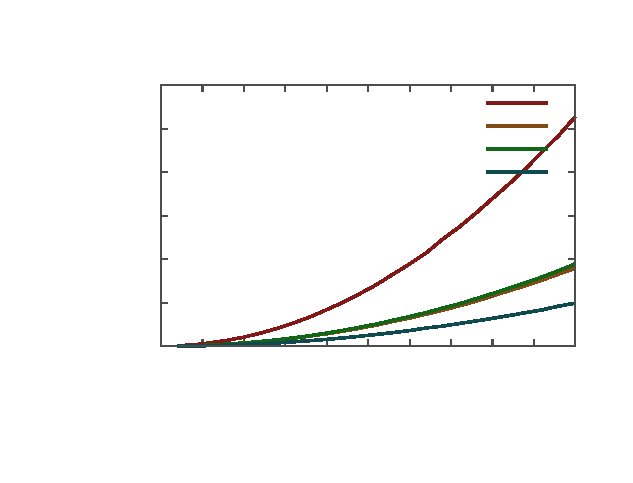
\includegraphics{./graficos/insercion-linux-opt}}%
    \gplfronttext
  \end{picture}%
\endgroup

	\end{center}

\subsection*{Representante de $\boldsymbol{O(n\log n)}$}
	\begin{center}
		% GNUPLOT: LaTeX picture with Postscript
\begingroup
  \makeatletter
  \providecommand\color[2][]{%
    \GenericError{(gnuplot) \space\space\space\@spaces}{%
      Package color not loaded in conjunction with
      terminal option `colourtext'%
    }{See the gnuplot documentation for explanation.%
    }{Either use 'blacktext' in gnuplot or load the package
      color.sty in LaTeX.}%
    \renewcommand\color[2][]{}%
  }%
  \providecommand\includegraphics[2][]{%
    \GenericError{(gnuplot) \space\space\space\@spaces}{%
      Package graphicx or graphics not loaded%
    }{See the gnuplot documentation for explanation.%
    }{The gnuplot epslatex terminal needs graphicx.sty or graphics.sty.}%
    \renewcommand\includegraphics[2][]{}%
  }%
  \providecommand\rotatebox[2]{#2}%
  \@ifundefined{ifGPcolor}{%
    \newif\ifGPcolor
    \GPcolortrue
  }{}%
  \@ifundefined{ifGPblacktext}{%
    \newif\ifGPblacktext
    \GPblacktextfalse
  }{}%
  % define a \g@addto@macro without @ in the name:
  \let\gplgaddtomacro\g@addto@macro
  % define empty templates for all commands taking text:
  \gdef\gplbacktext{}%
  \gdef\gplfronttext{}%
  \makeatother
  \ifGPblacktext
    % no textcolor at all
    \def\colorrgb#1{}%
    \def\colorgray#1{}%
  \else
    % gray or color?
    \ifGPcolor
      \def\colorrgb#1{\color[rgb]{#1}}%
      \def\colorgray#1{\color[gray]{#1}}%
      \expandafter\def\csname LTw\endcsname{\color{white}}%
      \expandafter\def\csname LTb\endcsname{\color{black}}%
      \expandafter\def\csname LTa\endcsname{\color{black}}%
      \expandafter\def\csname LT0\endcsname{\color[rgb]{1,0,0}}%
      \expandafter\def\csname LT1\endcsname{\color[rgb]{0,1,0}}%
      \expandafter\def\csname LT2\endcsname{\color[rgb]{0,0,1}}%
      \expandafter\def\csname LT3\endcsname{\color[rgb]{1,0,1}}%
      \expandafter\def\csname LT4\endcsname{\color[rgb]{0,1,1}}%
      \expandafter\def\csname LT5\endcsname{\color[rgb]{1,1,0}}%
      \expandafter\def\csname LT6\endcsname{\color[rgb]{0,0,0}}%
      \expandafter\def\csname LT7\endcsname{\color[rgb]{1,0.3,0}}%
      \expandafter\def\csname LT8\endcsname{\color[rgb]{0.5,0.5,0.5}}%
    \else
      % gray
      \def\colorrgb#1{\color{black}}%
      \def\colorgray#1{\color[gray]{#1}}%
      \expandafter\def\csname LTw\endcsname{\color{white}}%
      \expandafter\def\csname LTb\endcsname{\color{black}}%
      \expandafter\def\csname LTa\endcsname{\color{black}}%
      \expandafter\def\csname LT0\endcsname{\color{black}}%
      \expandafter\def\csname LT1\endcsname{\color{black}}%
      \expandafter\def\csname LT2\endcsname{\color{black}}%
      \expandafter\def\csname LT3\endcsname{\color{black}}%
      \expandafter\def\csname LT4\endcsname{\color{black}}%
      \expandafter\def\csname LT5\endcsname{\color{black}}%
      \expandafter\def\csname LT6\endcsname{\color{black}}%
      \expandafter\def\csname LT7\endcsname{\color{black}}%
      \expandafter\def\csname LT8\endcsname{\color{black}}%
    \fi
  \fi
    \setlength{\unitlength}{0.0500bp}%
    \ifx\gptboxheight\undefined%
      \newlength{\gptboxheight}%
      \newlength{\gptboxwidth}%
      \newsavebox{\gptboxtext}%
    \fi%
    \setlength{\fboxrule}{0.5pt}%
    \setlength{\fboxsep}{1pt}%
\begin{picture}(5760.00,4320.00)%
    \gplgaddtomacro\gplbacktext{%
      \colorrgb{0.30,0.30,0.30}%
      \put(1518,1246){\makebox(0,0)[r]{\strut{}$\textcolor{text}{0}$}}%
      \colorrgb{0.30,0.30,0.30}%
      \put(1518,1729){\makebox(0,0)[r]{\strut{}$\textcolor{text}{0.005}$}}%
      \colorrgb{0.30,0.30,0.30}%
      \put(1518,2211){\makebox(0,0)[r]{\strut{}$\textcolor{text}{0.01}$}}%
      \colorrgb{0.30,0.30,0.30}%
      \put(1518,2694){\makebox(0,0)[r]{\strut{}$\textcolor{text}{0.015}$}}%
      \colorrgb{0.30,0.30,0.30}%
      \put(1518,3176){\makebox(0,0)[r]{\strut{}$\textcolor{text}{0.02}$}}%
      \colorrgb{0.30,0.30,0.30}%
      \put(1518,3659){\makebox(0,0)[r]{\strut{}$\textcolor{text}{0.025}$}}%
      \colorrgb{0.30,0.30,0.30}%
      \put(1650,1114){\rotatebox{45}{\makebox(0,0)[r]{\strut{}$\textcolor{text}{0}$}}}%
      \colorrgb{0.30,0.30,0.30}%
      \put(2114,1114){\rotatebox{45}{\makebox(0,0)[r]{\strut{}$\textcolor{text}{20000}$}}}%
      \colorrgb{0.30,0.30,0.30}%
      \put(2578,1114){\rotatebox{45}{\makebox(0,0)[r]{\strut{}$\textcolor{text}{40000}$}}}%
      \colorrgb{0.30,0.30,0.30}%
      \put(3042,1114){\rotatebox{45}{\makebox(0,0)[r]{\strut{}$\textcolor{text}{60000}$}}}%
      \colorrgb{0.30,0.30,0.30}%
      \put(3507,1114){\rotatebox{45}{\makebox(0,0)[r]{\strut{}$\textcolor{text}{80000}$}}}%
      \colorrgb{0.30,0.30,0.30}%
      \put(3971,1114){\rotatebox{45}{\makebox(0,0)[r]{\strut{}$\textcolor{text}{100000}$}}}%
      \colorrgb{0.30,0.30,0.30}%
      \put(4435,1114){\rotatebox{45}{\makebox(0,0)[r]{\strut{}$\textcolor{text}{120000}$}}}%
      \colorrgb{0.30,0.30,0.30}%
      \put(4899,1114){\rotatebox{45}{\makebox(0,0)[r]{\strut{}$\textcolor{text}{140000}$}}}%
      \colorrgb{0.30,0.30,0.30}%
      \put(5363,1114){\rotatebox{45}{\makebox(0,0)[r]{\strut{}$\textcolor{text}{160000}$}}}%
    }%
    \gplgaddtomacro\gplfronttext{%
      \colorrgb{0.30,0.30,0.30}%
      \put(220,2452){\rotatebox{-270}{\makebox(0,0){\strut{}Tiempo de ejecución (s)}}}%
      \colorrgb{0.30,0.30,0.30}%
      \put(3506,220){\makebox(0,0){\strut{}Tamaño del vector (elementos)}}%
      \colorrgb{0.30,0.30,0.30}%
      \put(3506,3989){\makebox(0,0){\strut{}Comparación quicksort en macOS y Linux}}%
      \csname LTb\endcsname%
      \put(4376,3486){\makebox(0,0)[r]{\strut{}Linux}}%
      \csname LTb\endcsname%
      \put(4376,3266){\makebox(0,0)[r]{\strut{}Mac}}%
    }%
    \gplbacktext
    \put(0,0){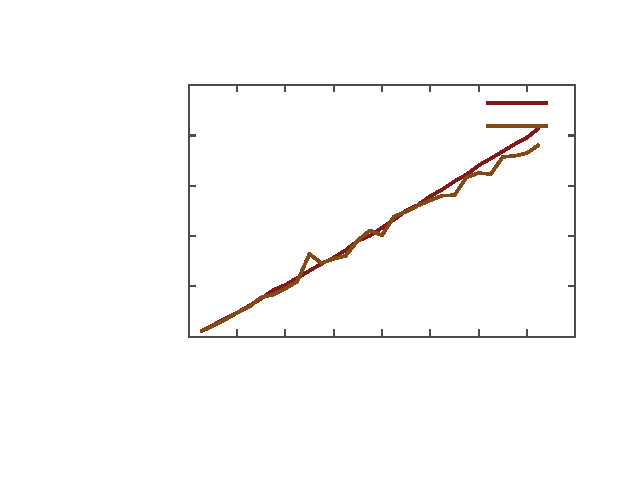
\includegraphics{./graficos/quicksort-maclinux}}%
    \gplfronttext
  \end{picture}%
\endgroup

	\end{center}

	\begin{center}
		% GNUPLOT: LaTeX picture with Postscript
\begingroup
  \makeatletter
  \providecommand\color[2][]{%
    \GenericError{(gnuplot) \space\space\space\@spaces}{%
      Package color not loaded in conjunction with
      terminal option `colourtext'%
    }{See the gnuplot documentation for explanation.%
    }{Either use 'blacktext' in gnuplot or load the package
      color.sty in LaTeX.}%
    \renewcommand\color[2][]{}%
  }%
  \providecommand\includegraphics[2][]{%
    \GenericError{(gnuplot) \space\space\space\@spaces}{%
      Package graphicx or graphics not loaded%
    }{See the gnuplot documentation for explanation.%
    }{The gnuplot epslatex terminal needs graphicx.sty or graphics.sty.}%
    \renewcommand\includegraphics[2][]{}%
  }%
  \providecommand\rotatebox[2]{#2}%
  \@ifundefined{ifGPcolor}{%
    \newif\ifGPcolor
    \GPcolortrue
  }{}%
  \@ifundefined{ifGPblacktext}{%
    \newif\ifGPblacktext
    \GPblacktextfalse
  }{}%
  % define a \g@addto@macro without @ in the name:
  \let\gplgaddtomacro\g@addto@macro
  % define empty templates for all commands taking text:
  \gdef\gplbacktext{}%
  \gdef\gplfronttext{}%
  \makeatother
  \ifGPblacktext
    % no textcolor at all
    \def\colorrgb#1{}%
    \def\colorgray#1{}%
  \else
    % gray or color?
    \ifGPcolor
      \def\colorrgb#1{\color[rgb]{#1}}%
      \def\colorgray#1{\color[gray]{#1}}%
      \expandafter\def\csname LTw\endcsname{\color{white}}%
      \expandafter\def\csname LTb\endcsname{\color{black}}%
      \expandafter\def\csname LTa\endcsname{\color{black}}%
      \expandafter\def\csname LT0\endcsname{\color[rgb]{1,0,0}}%
      \expandafter\def\csname LT1\endcsname{\color[rgb]{0,1,0}}%
      \expandafter\def\csname LT2\endcsname{\color[rgb]{0,0,1}}%
      \expandafter\def\csname LT3\endcsname{\color[rgb]{1,0,1}}%
      \expandafter\def\csname LT4\endcsname{\color[rgb]{0,1,1}}%
      \expandafter\def\csname LT5\endcsname{\color[rgb]{1,1,0}}%
      \expandafter\def\csname LT6\endcsname{\color[rgb]{0,0,0}}%
      \expandafter\def\csname LT7\endcsname{\color[rgb]{1,0.3,0}}%
      \expandafter\def\csname LT8\endcsname{\color[rgb]{0.5,0.5,0.5}}%
    \else
      % gray
      \def\colorrgb#1{\color{black}}%
      \def\colorgray#1{\color[gray]{#1}}%
      \expandafter\def\csname LTw\endcsname{\color{white}}%
      \expandafter\def\csname LTb\endcsname{\color{black}}%
      \expandafter\def\csname LTa\endcsname{\color{black}}%
      \expandafter\def\csname LT0\endcsname{\color{black}}%
      \expandafter\def\csname LT1\endcsname{\color{black}}%
      \expandafter\def\csname LT2\endcsname{\color{black}}%
      \expandafter\def\csname LT3\endcsname{\color{black}}%
      \expandafter\def\csname LT4\endcsname{\color{black}}%
      \expandafter\def\csname LT5\endcsname{\color{black}}%
      \expandafter\def\csname LT6\endcsname{\color{black}}%
      \expandafter\def\csname LT7\endcsname{\color{black}}%
      \expandafter\def\csname LT8\endcsname{\color{black}}%
    \fi
  \fi
    \setlength{\unitlength}{0.0500bp}%
    \ifx\gptboxheight\undefined%
      \newlength{\gptboxheight}%
      \newlength{\gptboxwidth}%
      \newsavebox{\gptboxtext}%
    \fi%
    \setlength{\fboxrule}{0.5pt}%
    \setlength{\fboxsep}{1pt}%
\begin{picture}(5760.00,4320.00)%
    \gplgaddtomacro\gplbacktext{%
      \colorrgb{0.30,0.30,0.30}%
      \put(1518,1246){\makebox(0,0)[r]{\strut{}$\textcolor{text}{0}$}}%
      \colorrgb{0.30,0.30,0.30}%
      \put(1518,1729){\makebox(0,0)[r]{\strut{}$\textcolor{text}{0.005}$}}%
      \colorrgb{0.30,0.30,0.30}%
      \put(1518,2211){\makebox(0,0)[r]{\strut{}$\textcolor{text}{0.01}$}}%
      \colorrgb{0.30,0.30,0.30}%
      \put(1518,2694){\makebox(0,0)[r]{\strut{}$\textcolor{text}{0.015}$}}%
      \colorrgb{0.30,0.30,0.30}%
      \put(1518,3176){\makebox(0,0)[r]{\strut{}$\textcolor{text}{0.02}$}}%
      \colorrgb{0.30,0.30,0.30}%
      \put(1518,3659){\makebox(0,0)[r]{\strut{}$\textcolor{text}{0.025}$}}%
      \colorrgb{0.30,0.30,0.30}%
      \put(1650,1114){\rotatebox{45}{\makebox(0,0)[r]{\strut{}$\textcolor{text}{0}$}}}%
      \colorrgb{0.30,0.30,0.30}%
      \put(2114,1114){\rotatebox{45}{\makebox(0,0)[r]{\strut{}$\textcolor{text}{20000}$}}}%
      \colorrgb{0.30,0.30,0.30}%
      \put(2578,1114){\rotatebox{45}{\makebox(0,0)[r]{\strut{}$\textcolor{text}{40000}$}}}%
      \colorrgb{0.30,0.30,0.30}%
      \put(3042,1114){\rotatebox{45}{\makebox(0,0)[r]{\strut{}$\textcolor{text}{60000}$}}}%
      \colorrgb{0.30,0.30,0.30}%
      \put(3507,1114){\rotatebox{45}{\makebox(0,0)[r]{\strut{}$\textcolor{text}{80000}$}}}%
      \colorrgb{0.30,0.30,0.30}%
      \put(3971,1114){\rotatebox{45}{\makebox(0,0)[r]{\strut{}$\textcolor{text}{100000}$}}}%
      \colorrgb{0.30,0.30,0.30}%
      \put(4435,1114){\rotatebox{45}{\makebox(0,0)[r]{\strut{}$\textcolor{text}{120000}$}}}%
      \colorrgb{0.30,0.30,0.30}%
      \put(4899,1114){\rotatebox{45}{\makebox(0,0)[r]{\strut{}$\textcolor{text}{140000}$}}}%
      \colorrgb{0.30,0.30,0.30}%
      \put(5363,1114){\rotatebox{45}{\makebox(0,0)[r]{\strut{}$\textcolor{text}{160000}$}}}%
    }%
    \gplgaddtomacro\gplfronttext{%
      \colorrgb{0.30,0.30,0.30}%
      \put(220,2452){\rotatebox{-270}{\makebox(0,0){\strut{}Tiempo de ejecución (s)}}}%
      \colorrgb{0.30,0.30,0.30}%
      \put(3506,220){\makebox(0,0){\strut{}Tamaño del vector (elementos)}}%
      \colorrgb{0.30,0.30,0.30}%
      \put(3506,3989){\makebox(0,0){\strut{}Comparación quicksort en Linux con distinta optimización}}%
      \csname LTb\endcsname%
      \put(4376,3486){\makebox(0,0)[r]{\strut{}O0}}%
      \csname LTb\endcsname%
      \put(4376,3266){\makebox(0,0)[r]{\strut{}O1}}%
      \csname LTb\endcsname%
      \put(4376,3046){\makebox(0,0)[r]{\strut{}O2}}%
      \csname LTb\endcsname%
      \put(4376,2826){\makebox(0,0)[r]{\strut{}O3}}%
    }%
    \gplbacktext
    \put(0,0){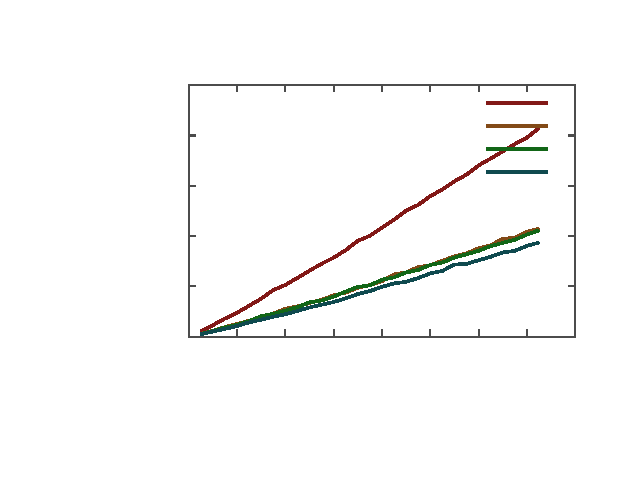
\includegraphics{./graficos/quicksort-linux-opt}}%
    \gplfronttext
  \end{picture}%
\endgroup

	\end{center}

\subsection*{Representante de $\boldsymbol{O(n^3)}$}
	\begin{center}
		% GNUPLOT: LaTeX picture with Postscript
\begingroup
  \makeatletter
  \providecommand\color[2][]{%
    \GenericError{(gnuplot) \space\space\space\@spaces}{%
      Package color not loaded in conjunction with
      terminal option `colourtext'%
    }{See the gnuplot documentation for explanation.%
    }{Either use 'blacktext' in gnuplot or load the package
      color.sty in LaTeX.}%
    \renewcommand\color[2][]{}%
  }%
  \providecommand\includegraphics[2][]{%
    \GenericError{(gnuplot) \space\space\space\@spaces}{%
      Package graphicx or graphics not loaded%
    }{See the gnuplot documentation for explanation.%
    }{The gnuplot epslatex terminal needs graphicx.sty or graphics.sty.}%
    \renewcommand\includegraphics[2][]{}%
  }%
  \providecommand\rotatebox[2]{#2}%
  \@ifundefined{ifGPcolor}{%
    \newif\ifGPcolor
    \GPcolortrue
  }{}%
  \@ifundefined{ifGPblacktext}{%
    \newif\ifGPblacktext
    \GPblacktextfalse
  }{}%
  % define a \g@addto@macro without @ in the name:
  \let\gplgaddtomacro\g@addto@macro
  % define empty templates for all commands taking text:
  \gdef\gplbacktext{}%
  \gdef\gplfronttext{}%
  \makeatother
  \ifGPblacktext
    % no textcolor at all
    \def\colorrgb#1{}%
    \def\colorgray#1{}%
  \else
    % gray or color?
    \ifGPcolor
      \def\colorrgb#1{\color[rgb]{#1}}%
      \def\colorgray#1{\color[gray]{#1}}%
      \expandafter\def\csname LTw\endcsname{\color{white}}%
      \expandafter\def\csname LTb\endcsname{\color{black}}%
      \expandafter\def\csname LTa\endcsname{\color{black}}%
      \expandafter\def\csname LT0\endcsname{\color[rgb]{1,0,0}}%
      \expandafter\def\csname LT1\endcsname{\color[rgb]{0,1,0}}%
      \expandafter\def\csname LT2\endcsname{\color[rgb]{0,0,1}}%
      \expandafter\def\csname LT3\endcsname{\color[rgb]{1,0,1}}%
      \expandafter\def\csname LT4\endcsname{\color[rgb]{0,1,1}}%
      \expandafter\def\csname LT5\endcsname{\color[rgb]{1,1,0}}%
      \expandafter\def\csname LT6\endcsname{\color[rgb]{0,0,0}}%
      \expandafter\def\csname LT7\endcsname{\color[rgb]{1,0.3,0}}%
      \expandafter\def\csname LT8\endcsname{\color[rgb]{0.5,0.5,0.5}}%
    \else
      % gray
      \def\colorrgb#1{\color{black}}%
      \def\colorgray#1{\color[gray]{#1}}%
      \expandafter\def\csname LTw\endcsname{\color{white}}%
      \expandafter\def\csname LTb\endcsname{\color{black}}%
      \expandafter\def\csname LTa\endcsname{\color{black}}%
      \expandafter\def\csname LT0\endcsname{\color{black}}%
      \expandafter\def\csname LT1\endcsname{\color{black}}%
      \expandafter\def\csname LT2\endcsname{\color{black}}%
      \expandafter\def\csname LT3\endcsname{\color{black}}%
      \expandafter\def\csname LT4\endcsname{\color{black}}%
      \expandafter\def\csname LT5\endcsname{\color{black}}%
      \expandafter\def\csname LT6\endcsname{\color{black}}%
      \expandafter\def\csname LT7\endcsname{\color{black}}%
      \expandafter\def\csname LT8\endcsname{\color{black}}%
    \fi
  \fi
    \setlength{\unitlength}{0.0500bp}%
    \ifx\gptboxheight\undefined%
      \newlength{\gptboxheight}%
      \newlength{\gptboxwidth}%
      \newsavebox{\gptboxtext}%
    \fi%
    \setlength{\fboxrule}{0.5pt}%
    \setlength{\fboxsep}{1pt}%
\begin{picture}(5760.00,4320.00)%
    \gplgaddtomacro\gplbacktext{%
      \colorrgb{0.30,0.30,0.30}%
      \put(1122,1060){\makebox(0,0)[r]{\strut{}$\textcolor{text}{0}$}}%
      \colorrgb{0.30,0.30,0.30}%
      \put(1122,1320){\makebox(0,0)[r]{\strut{}$\textcolor{text}{2}$}}%
      \colorrgb{0.30,0.30,0.30}%
      \put(1122,1580){\makebox(0,0)[r]{\strut{}$\textcolor{text}{4}$}}%
      \colorrgb{0.30,0.30,0.30}%
      \put(1122,1840){\makebox(0,0)[r]{\strut{}$\textcolor{text}{6}$}}%
      \colorrgb{0.30,0.30,0.30}%
      \put(1122,2100){\makebox(0,0)[r]{\strut{}$\textcolor{text}{8}$}}%
      \colorrgb{0.30,0.30,0.30}%
      \put(1122,2360){\makebox(0,0)[r]{\strut{}$\textcolor{text}{10}$}}%
      \colorrgb{0.30,0.30,0.30}%
      \put(1122,2619){\makebox(0,0)[r]{\strut{}$\textcolor{text}{12}$}}%
      \colorrgb{0.30,0.30,0.30}%
      \put(1122,2879){\makebox(0,0)[r]{\strut{}$\textcolor{text}{14}$}}%
      \colorrgb{0.30,0.30,0.30}%
      \put(1122,3139){\makebox(0,0)[r]{\strut{}$\textcolor{text}{16}$}}%
      \colorrgb{0.30,0.30,0.30}%
      \put(1122,3399){\makebox(0,0)[r]{\strut{}$\textcolor{text}{18}$}}%
      \colorrgb{0.30,0.30,0.30}%
      \put(1122,3659){\makebox(0,0)[r]{\strut{}$\textcolor{text}{20}$}}%
      \colorrgb{0.30,0.30,0.30}%
      \put(1254,928){\rotatebox{45}{\makebox(0,0)[r]{\strut{}$\textcolor{text}{0}$}}}%
      \colorrgb{0.30,0.30,0.30}%
      \put(1768,928){\rotatebox{45}{\makebox(0,0)[r]{\strut{}$\textcolor{text}{200}$}}}%
      \colorrgb{0.30,0.30,0.30}%
      \put(2281,928){\rotatebox{45}{\makebox(0,0)[r]{\strut{}$\textcolor{text}{400}$}}}%
      \colorrgb{0.30,0.30,0.30}%
      \put(2795,928){\rotatebox{45}{\makebox(0,0)[r]{\strut{}$\textcolor{text}{600}$}}}%
      \colorrgb{0.30,0.30,0.30}%
      \put(3309,928){\rotatebox{45}{\makebox(0,0)[r]{\strut{}$\textcolor{text}{800}$}}}%
      \colorrgb{0.30,0.30,0.30}%
      \put(3822,928){\rotatebox{45}{\makebox(0,0)[r]{\strut{}$\textcolor{text}{1000}$}}}%
      \colorrgb{0.30,0.30,0.30}%
      \put(4336,928){\rotatebox{45}{\makebox(0,0)[r]{\strut{}$\textcolor{text}{1200}$}}}%
      \colorrgb{0.30,0.30,0.30}%
      \put(4849,928){\rotatebox{45}{\makebox(0,0)[r]{\strut{}$\textcolor{text}{1400}$}}}%
      \colorrgb{0.30,0.30,0.30}%
      \put(5363,928){\rotatebox{45}{\makebox(0,0)[r]{\strut{}$\textcolor{text}{1600}$}}}%
    }%
    \gplgaddtomacro\gplfronttext{%
      \colorrgb{0.30,0.30,0.30}%
      \put(220,2359){\rotatebox{-270}{\makebox(0,0){\strut{}Tiempo de ejecución (s)}}}%
      \colorrgb{0.30,0.30,0.30}%
      \put(3308,220){\makebox(0,0){\strut{}Tamaño del vector (elementos)}}%
      \colorrgb{0.30,0.30,0.30}%
      \put(3308,3989){\makebox(0,0){\strut{}Comparación floyd en macOS y Linux}}%
      \csname LTb\endcsname%
      \put(4376,3486){\makebox(0,0)[r]{\strut{}Linux}}%
      \csname LTb\endcsname%
      \put(4376,3266){\makebox(0,0)[r]{\strut{}Mac}}%
    }%
    \gplbacktext
    \put(0,0){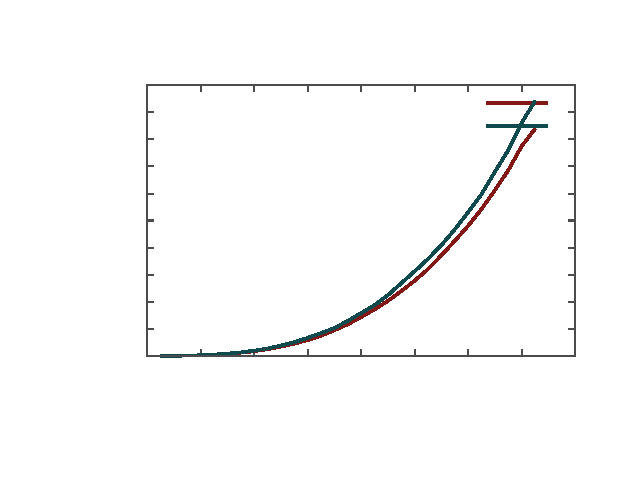
\includegraphics{./graficos/floyd-maclinux}}%
    \gplfronttext
  \end{picture}%
\endgroup

	\end{center}

	\begin{center}
		% GNUPLOT: LaTeX picture with Postscript
\begingroup
  \makeatletter
  \providecommand\color[2][]{%
    \GenericError{(gnuplot) \space\space\space\@spaces}{%
      Package color not loaded in conjunction with
      terminal option `colourtext'%
    }{See the gnuplot documentation for explanation.%
    }{Either use 'blacktext' in gnuplot or load the package
      color.sty in LaTeX.}%
    \renewcommand\color[2][]{}%
  }%
  \providecommand\includegraphics[2][]{%
    \GenericError{(gnuplot) \space\space\space\@spaces}{%
      Package graphicx or graphics not loaded%
    }{See the gnuplot documentation for explanation.%
    }{The gnuplot epslatex terminal needs graphicx.sty or graphics.sty.}%
    \renewcommand\includegraphics[2][]{}%
  }%
  \providecommand\rotatebox[2]{#2}%
  \@ifundefined{ifGPcolor}{%
    \newif\ifGPcolor
    \GPcolortrue
  }{}%
  \@ifundefined{ifGPblacktext}{%
    \newif\ifGPblacktext
    \GPblacktextfalse
  }{}%
  % define a \g@addto@macro without @ in the name:
  \let\gplgaddtomacro\g@addto@macro
  % define empty templates for all commands taking text:
  \gdef\gplbacktext{}%
  \gdef\gplfronttext{}%
  \makeatother
  \ifGPblacktext
    % no textcolor at all
    \def\colorrgb#1{}%
    \def\colorgray#1{}%
  \else
    % gray or color?
    \ifGPcolor
      \def\colorrgb#1{\color[rgb]{#1}}%
      \def\colorgray#1{\color[gray]{#1}}%
      \expandafter\def\csname LTw\endcsname{\color{white}}%
      \expandafter\def\csname LTb\endcsname{\color{black}}%
      \expandafter\def\csname LTa\endcsname{\color{black}}%
      \expandafter\def\csname LT0\endcsname{\color[rgb]{1,0,0}}%
      \expandafter\def\csname LT1\endcsname{\color[rgb]{0,1,0}}%
      \expandafter\def\csname LT2\endcsname{\color[rgb]{0,0,1}}%
      \expandafter\def\csname LT3\endcsname{\color[rgb]{1,0,1}}%
      \expandafter\def\csname LT4\endcsname{\color[rgb]{0,1,1}}%
      \expandafter\def\csname LT5\endcsname{\color[rgb]{1,1,0}}%
      \expandafter\def\csname LT6\endcsname{\color[rgb]{0,0,0}}%
      \expandafter\def\csname LT7\endcsname{\color[rgb]{1,0.3,0}}%
      \expandafter\def\csname LT8\endcsname{\color[rgb]{0.5,0.5,0.5}}%
    \else
      % gray
      \def\colorrgb#1{\color{black}}%
      \def\colorgray#1{\color[gray]{#1}}%
      \expandafter\def\csname LTw\endcsname{\color{white}}%
      \expandafter\def\csname LTb\endcsname{\color{black}}%
      \expandafter\def\csname LTa\endcsname{\color{black}}%
      \expandafter\def\csname LT0\endcsname{\color{black}}%
      \expandafter\def\csname LT1\endcsname{\color{black}}%
      \expandafter\def\csname LT2\endcsname{\color{black}}%
      \expandafter\def\csname LT3\endcsname{\color{black}}%
      \expandafter\def\csname LT4\endcsname{\color{black}}%
      \expandafter\def\csname LT5\endcsname{\color{black}}%
      \expandafter\def\csname LT6\endcsname{\color{black}}%
      \expandafter\def\csname LT7\endcsname{\color{black}}%
      \expandafter\def\csname LT8\endcsname{\color{black}}%
    \fi
  \fi
    \setlength{\unitlength}{0.0500bp}%
    \ifx\gptboxheight\undefined%
      \newlength{\gptboxheight}%
      \newlength{\gptboxwidth}%
      \newsavebox{\gptboxtext}%
    \fi%
    \setlength{\fboxrule}{0.5pt}%
    \setlength{\fboxsep}{1pt}%
\begin{picture}(5760.00,4320.00)%
    \gplgaddtomacro\gplbacktext{%
      \colorrgb{0.30,0.30,0.30}%
      \put(1122,1060){\makebox(0,0)[r]{\strut{}$\textcolor{text}{0}$}}%
      \colorrgb{0.30,0.30,0.30}%
      \put(1122,1349){\makebox(0,0)[r]{\strut{}$\textcolor{text}{2}$}}%
      \colorrgb{0.30,0.30,0.30}%
      \put(1122,1638){\makebox(0,0)[r]{\strut{}$\textcolor{text}{4}$}}%
      \colorrgb{0.30,0.30,0.30}%
      \put(1122,1926){\makebox(0,0)[r]{\strut{}$\textcolor{text}{6}$}}%
      \colorrgb{0.30,0.30,0.30}%
      \put(1122,2215){\makebox(0,0)[r]{\strut{}$\textcolor{text}{8}$}}%
      \colorrgb{0.30,0.30,0.30}%
      \put(1122,2504){\makebox(0,0)[r]{\strut{}$\textcolor{text}{10}$}}%
      \colorrgb{0.30,0.30,0.30}%
      \put(1122,2793){\makebox(0,0)[r]{\strut{}$\textcolor{text}{12}$}}%
      \colorrgb{0.30,0.30,0.30}%
      \put(1122,3081){\makebox(0,0)[r]{\strut{}$\textcolor{text}{14}$}}%
      \colorrgb{0.30,0.30,0.30}%
      \put(1122,3370){\makebox(0,0)[r]{\strut{}$\textcolor{text}{16}$}}%
      \colorrgb{0.30,0.30,0.30}%
      \put(1122,3659){\makebox(0,0)[r]{\strut{}$\textcolor{text}{18}$}}%
      \colorrgb{0.30,0.30,0.30}%
      \put(1254,928){\rotatebox{45}{\makebox(0,0)[r]{\strut{}$\textcolor{text}{0}$}}}%
      \colorrgb{0.30,0.30,0.30}%
      \put(1768,928){\rotatebox{45}{\makebox(0,0)[r]{\strut{}$\textcolor{text}{200}$}}}%
      \colorrgb{0.30,0.30,0.30}%
      \put(2281,928){\rotatebox{45}{\makebox(0,0)[r]{\strut{}$\textcolor{text}{400}$}}}%
      \colorrgb{0.30,0.30,0.30}%
      \put(2795,928){\rotatebox{45}{\makebox(0,0)[r]{\strut{}$\textcolor{text}{600}$}}}%
      \colorrgb{0.30,0.30,0.30}%
      \put(3309,928){\rotatebox{45}{\makebox(0,0)[r]{\strut{}$\textcolor{text}{800}$}}}%
      \colorrgb{0.30,0.30,0.30}%
      \put(3822,928){\rotatebox{45}{\makebox(0,0)[r]{\strut{}$\textcolor{text}{1000}$}}}%
      \colorrgb{0.30,0.30,0.30}%
      \put(4336,928){\rotatebox{45}{\makebox(0,0)[r]{\strut{}$\textcolor{text}{1200}$}}}%
      \colorrgb{0.30,0.30,0.30}%
      \put(4849,928){\rotatebox{45}{\makebox(0,0)[r]{\strut{}$\textcolor{text}{1400}$}}}%
      \colorrgb{0.30,0.30,0.30}%
      \put(5363,928){\rotatebox{45}{\makebox(0,0)[r]{\strut{}$\textcolor{text}{1600}$}}}%
    }%
    \gplgaddtomacro\gplfronttext{%
      \colorrgb{0.30,0.30,0.30}%
      \put(220,2359){\rotatebox{-270}{\makebox(0,0){\strut{}Tiempo de ejecución (s)}}}%
      \colorrgb{0.30,0.30,0.30}%
      \put(3308,220){\makebox(0,0){\strut{}Tamaño del vector (elementos)}}%
      \colorrgb{0.30,0.30,0.30}%
      \put(3308,3989){\makebox(0,0){\strut{}Comparación floyd en Linux con distinta optimización}}%
      \csname LTb\endcsname%
      \put(4376,3486){\makebox(0,0)[r]{\strut{}O0}}%
      \csname LTb\endcsname%
      \put(4376,3266){\makebox(0,0)[r]{\strut{}O1}}%
      \csname LTb\endcsname%
      \put(4376,3046){\makebox(0,0)[r]{\strut{}O2}}%
      \csname LTb\endcsname%
      \put(4376,2826){\makebox(0,0)[r]{\strut{}O3}}%
    }%
    \gplbacktext
    \put(0,0){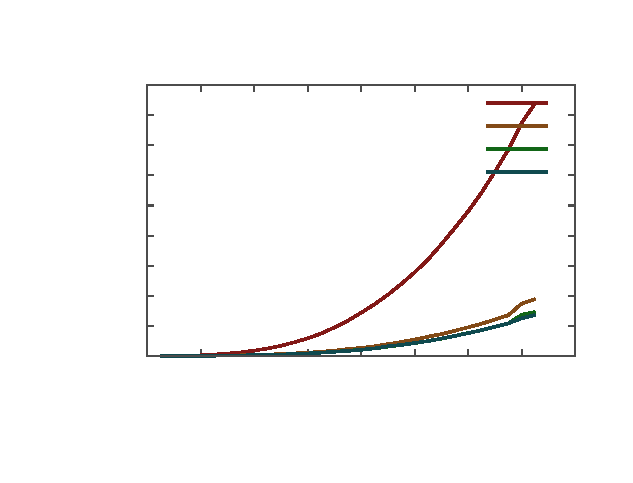
\includegraphics{./graficos/floyd-linux-opt}}%
    \gplfronttext
  \end{picture}%
\endgroup

	\end{center}

\subsection*{Representante de $\boldsymbol{O(2^n)}$}
	\begin{center}
		% GNUPLOT: LaTeX picture with Postscript
\begingroup
  \makeatletter
  \providecommand\color[2][]{%
    \GenericError{(gnuplot) \space\space\space\@spaces}{%
      Package color not loaded in conjunction with
      terminal option `colourtext'%
    }{See the gnuplot documentation for explanation.%
    }{Either use 'blacktext' in gnuplot or load the package
      color.sty in LaTeX.}%
    \renewcommand\color[2][]{}%
  }%
  \providecommand\includegraphics[2][]{%
    \GenericError{(gnuplot) \space\space\space\@spaces}{%
      Package graphicx or graphics not loaded%
    }{See the gnuplot documentation for explanation.%
    }{The gnuplot epslatex terminal needs graphicx.sty or graphics.sty.}%
    \renewcommand\includegraphics[2][]{}%
  }%
  \providecommand\rotatebox[2]{#2}%
  \@ifundefined{ifGPcolor}{%
    \newif\ifGPcolor
    \GPcolortrue
  }{}%
  \@ifundefined{ifGPblacktext}{%
    \newif\ifGPblacktext
    \GPblacktextfalse
  }{}%
  % define a \g@addto@macro without @ in the name:
  \let\gplgaddtomacro\g@addto@macro
  % define empty templates for all commands taking text:
  \gdef\gplbacktext{}%
  \gdef\gplfronttext{}%
  \makeatother
  \ifGPblacktext
    % no textcolor at all
    \def\colorrgb#1{}%
    \def\colorgray#1{}%
  \else
    % gray or color?
    \ifGPcolor
      \def\colorrgb#1{\color[rgb]{#1}}%
      \def\colorgray#1{\color[gray]{#1}}%
      \expandafter\def\csname LTw\endcsname{\color{white}}%
      \expandafter\def\csname LTb\endcsname{\color{black}}%
      \expandafter\def\csname LTa\endcsname{\color{black}}%
      \expandafter\def\csname LT0\endcsname{\color[rgb]{1,0,0}}%
      \expandafter\def\csname LT1\endcsname{\color[rgb]{0,1,0}}%
      \expandafter\def\csname LT2\endcsname{\color[rgb]{0,0,1}}%
      \expandafter\def\csname LT3\endcsname{\color[rgb]{1,0,1}}%
      \expandafter\def\csname LT4\endcsname{\color[rgb]{0,1,1}}%
      \expandafter\def\csname LT5\endcsname{\color[rgb]{1,1,0}}%
      \expandafter\def\csname LT6\endcsname{\color[rgb]{0,0,0}}%
      \expandafter\def\csname LT7\endcsname{\color[rgb]{1,0.3,0}}%
      \expandafter\def\csname LT8\endcsname{\color[rgb]{0.5,0.5,0.5}}%
    \else
      % gray
      \def\colorrgb#1{\color{black}}%
      \def\colorgray#1{\color[gray]{#1}}%
      \expandafter\def\csname LTw\endcsname{\color{white}}%
      \expandafter\def\csname LTb\endcsname{\color{black}}%
      \expandafter\def\csname LTa\endcsname{\color{black}}%
      \expandafter\def\csname LT0\endcsname{\color{black}}%
      \expandafter\def\csname LT1\endcsname{\color{black}}%
      \expandafter\def\csname LT2\endcsname{\color{black}}%
      \expandafter\def\csname LT3\endcsname{\color{black}}%
      \expandafter\def\csname LT4\endcsname{\color{black}}%
      \expandafter\def\csname LT5\endcsname{\color{black}}%
      \expandafter\def\csname LT6\endcsname{\color{black}}%
      \expandafter\def\csname LT7\endcsname{\color{black}}%
      \expandafter\def\csname LT8\endcsname{\color{black}}%
    \fi
  \fi
    \setlength{\unitlength}{0.0500bp}%
    \ifx\gptboxheight\undefined%
      \newlength{\gptboxheight}%
      \newlength{\gptboxwidth}%
      \newsavebox{\gptboxtext}%
    \fi%
    \setlength{\fboxrule}{0.5pt}%
    \setlength{\fboxsep}{1pt}%
\begin{picture}(5760.00,4320.00)%
    \gplgaddtomacro\gplbacktext{%
      \colorrgb{0.30,0.30,0.30}%
      \put(990,873){\makebox(0,0)[r]{\strut{}$\textcolor{text}{0}$}}%
      \colorrgb{0.30,0.30,0.30}%
      \put(990,1271){\makebox(0,0)[r]{\strut{}$\textcolor{text}{1}$}}%
      \colorrgb{0.30,0.30,0.30}%
      \put(990,1669){\makebox(0,0)[r]{\strut{}$\textcolor{text}{2}$}}%
      \colorrgb{0.30,0.30,0.30}%
      \put(990,2067){\makebox(0,0)[r]{\strut{}$\textcolor{text}{3}$}}%
      \colorrgb{0.30,0.30,0.30}%
      \put(990,2465){\makebox(0,0)[r]{\strut{}$\textcolor{text}{4}$}}%
      \colorrgb{0.30,0.30,0.30}%
      \put(990,2863){\makebox(0,0)[r]{\strut{}$\textcolor{text}{5}$}}%
      \colorrgb{0.30,0.30,0.30}%
      \put(990,3261){\makebox(0,0)[r]{\strut{}$\textcolor{text}{6}$}}%
      \colorrgb{0.30,0.30,0.30}%
      \put(990,3659){\makebox(0,0)[r]{\strut{}$\textcolor{text}{7}$}}%
      \colorrgb{0.30,0.30,0.30}%
      \put(1122,741){\rotatebox{45}{\makebox(0,0)[r]{\strut{}$\textcolor{text}{5}$}}}%
      \colorrgb{0.30,0.30,0.30}%
      \put(1970,741){\rotatebox{45}{\makebox(0,0)[r]{\strut{}$\textcolor{text}{10}$}}}%
      \colorrgb{0.30,0.30,0.30}%
      \put(2818,741){\rotatebox{45}{\makebox(0,0)[r]{\strut{}$\textcolor{text}{15}$}}}%
      \colorrgb{0.30,0.30,0.30}%
      \put(3667,741){\rotatebox{45}{\makebox(0,0)[r]{\strut{}$\textcolor{text}{20}$}}}%
      \colorrgb{0.30,0.30,0.30}%
      \put(4515,741){\rotatebox{45}{\makebox(0,0)[r]{\strut{}$\textcolor{text}{25}$}}}%
      \colorrgb{0.30,0.30,0.30}%
      \put(5363,741){\rotatebox{45}{\makebox(0,0)[r]{\strut{}$\textcolor{text}{30}$}}}%
    }%
    \gplgaddtomacro\gplfronttext{%
      \colorrgb{0.30,0.30,0.30}%
      \put(220,2266){\rotatebox{-270}{\makebox(0,0){\strut{}Tiempo de ejecución (s)}}}%
      \colorrgb{0.30,0.30,0.30}%
      \put(3242,220){\makebox(0,0){\strut{}Tamaño del vector (elementos)}}%
      \colorrgb{0.30,0.30,0.30}%
      \put(3242,3989){\makebox(0,0){\strut{}Comparación hanoi en macOS y Linux}}%
      \csname LTb\endcsname%
      \put(4376,3486){\makebox(0,0)[r]{\strut{}Linux}}%
      \csname LTb\endcsname%
      \put(4376,3266){\makebox(0,0)[r]{\strut{}Mac}}%
    }%
    \gplbacktext
    \put(0,0){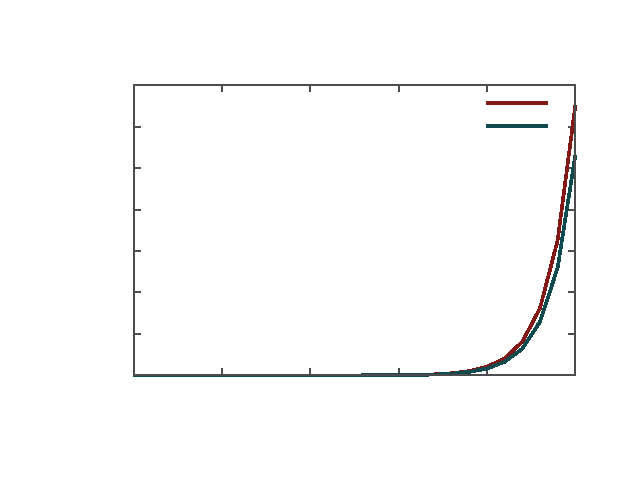
\includegraphics{./graficos/hanoi-maclinux}}%
    \gplfronttext
  \end{picture}%
\endgroup

	\end{center}

	\begin{center}
		% GNUPLOT: LaTeX picture with Postscript
\begingroup
  \makeatletter
  \providecommand\color[2][]{%
    \GenericError{(gnuplot) \space\space\space\@spaces}{%
      Package color not loaded in conjunction with
      terminal option `colourtext'%
    }{See the gnuplot documentation for explanation.%
    }{Either use 'blacktext' in gnuplot or load the package
      color.sty in LaTeX.}%
    \renewcommand\color[2][]{}%
  }%
  \providecommand\includegraphics[2][]{%
    \GenericError{(gnuplot) \space\space\space\@spaces}{%
      Package graphicx or graphics not loaded%
    }{See the gnuplot documentation for explanation.%
    }{The gnuplot epslatex terminal needs graphicx.sty or graphics.sty.}%
    \renewcommand\includegraphics[2][]{}%
  }%
  \providecommand\rotatebox[2]{#2}%
  \@ifundefined{ifGPcolor}{%
    \newif\ifGPcolor
    \GPcolortrue
  }{}%
  \@ifundefined{ifGPblacktext}{%
    \newif\ifGPblacktext
    \GPblacktextfalse
  }{}%
  % define a \g@addto@macro without @ in the name:
  \let\gplgaddtomacro\g@addto@macro
  % define empty templates for all commands taking text:
  \gdef\gplbacktext{}%
  \gdef\gplfronttext{}%
  \makeatother
  \ifGPblacktext
    % no textcolor at all
    \def\colorrgb#1{}%
    \def\colorgray#1{}%
  \else
    % gray or color?
    \ifGPcolor
      \def\colorrgb#1{\color[rgb]{#1}}%
      \def\colorgray#1{\color[gray]{#1}}%
      \expandafter\def\csname LTw\endcsname{\color{white}}%
      \expandafter\def\csname LTb\endcsname{\color{black}}%
      \expandafter\def\csname LTa\endcsname{\color{black}}%
      \expandafter\def\csname LT0\endcsname{\color[rgb]{1,0,0}}%
      \expandafter\def\csname LT1\endcsname{\color[rgb]{0,1,0}}%
      \expandafter\def\csname LT2\endcsname{\color[rgb]{0,0,1}}%
      \expandafter\def\csname LT3\endcsname{\color[rgb]{1,0,1}}%
      \expandafter\def\csname LT4\endcsname{\color[rgb]{0,1,1}}%
      \expandafter\def\csname LT5\endcsname{\color[rgb]{1,1,0}}%
      \expandafter\def\csname LT6\endcsname{\color[rgb]{0,0,0}}%
      \expandafter\def\csname LT7\endcsname{\color[rgb]{1,0.3,0}}%
      \expandafter\def\csname LT8\endcsname{\color[rgb]{0.5,0.5,0.5}}%
    \else
      % gray
      \def\colorrgb#1{\color{black}}%
      \def\colorgray#1{\color[gray]{#1}}%
      \expandafter\def\csname LTw\endcsname{\color{white}}%
      \expandafter\def\csname LTb\endcsname{\color{black}}%
      \expandafter\def\csname LTa\endcsname{\color{black}}%
      \expandafter\def\csname LT0\endcsname{\color{black}}%
      \expandafter\def\csname LT1\endcsname{\color{black}}%
      \expandafter\def\csname LT2\endcsname{\color{black}}%
      \expandafter\def\csname LT3\endcsname{\color{black}}%
      \expandafter\def\csname LT4\endcsname{\color{black}}%
      \expandafter\def\csname LT5\endcsname{\color{black}}%
      \expandafter\def\csname LT6\endcsname{\color{black}}%
      \expandafter\def\csname LT7\endcsname{\color{black}}%
      \expandafter\def\csname LT8\endcsname{\color{black}}%
    \fi
  \fi
    \setlength{\unitlength}{0.0500bp}%
    \ifx\gptboxheight\undefined%
      \newlength{\gptboxheight}%
      \newlength{\gptboxwidth}%
      \newsavebox{\gptboxtext}%
    \fi%
    \setlength{\fboxrule}{0.5pt}%
    \setlength{\fboxsep}{1pt}%
\begin{picture}(5760.00,4320.00)%
    \gplgaddtomacro\gplbacktext{%
      \colorrgb{0.30,0.30,0.30}%
      \put(990,873){\makebox(0,0)[r]{\strut{}$\textcolor{text}{0}$}}%
      \colorrgb{0.30,0.30,0.30}%
      \put(990,1271){\makebox(0,0)[r]{\strut{}$\textcolor{text}{1}$}}%
      \colorrgb{0.30,0.30,0.30}%
      \put(990,1669){\makebox(0,0)[r]{\strut{}$\textcolor{text}{2}$}}%
      \colorrgb{0.30,0.30,0.30}%
      \put(990,2067){\makebox(0,0)[r]{\strut{}$\textcolor{text}{3}$}}%
      \colorrgb{0.30,0.30,0.30}%
      \put(990,2465){\makebox(0,0)[r]{\strut{}$\textcolor{text}{4}$}}%
      \colorrgb{0.30,0.30,0.30}%
      \put(990,2863){\makebox(0,0)[r]{\strut{}$\textcolor{text}{5}$}}%
      \colorrgb{0.30,0.30,0.30}%
      \put(990,3261){\makebox(0,0)[r]{\strut{}$\textcolor{text}{6}$}}%
      \colorrgb{0.30,0.30,0.30}%
      \put(990,3659){\makebox(0,0)[r]{\strut{}$\textcolor{text}{7}$}}%
      \colorrgb{0.30,0.30,0.30}%
      \put(1122,741){\rotatebox{45}{\makebox(0,0)[r]{\strut{}$\textcolor{text}{5}$}}}%
      \colorrgb{0.30,0.30,0.30}%
      \put(1970,741){\rotatebox{45}{\makebox(0,0)[r]{\strut{}$\textcolor{text}{10}$}}}%
      \colorrgb{0.30,0.30,0.30}%
      \put(2818,741){\rotatebox{45}{\makebox(0,0)[r]{\strut{}$\textcolor{text}{15}$}}}%
      \colorrgb{0.30,0.30,0.30}%
      \put(3667,741){\rotatebox{45}{\makebox(0,0)[r]{\strut{}$\textcolor{text}{20}$}}}%
      \colorrgb{0.30,0.30,0.30}%
      \put(4515,741){\rotatebox{45}{\makebox(0,0)[r]{\strut{}$\textcolor{text}{25}$}}}%
      \colorrgb{0.30,0.30,0.30}%
      \put(5363,741){\rotatebox{45}{\makebox(0,0)[r]{\strut{}$\textcolor{text}{30}$}}}%
    }%
    \gplgaddtomacro\gplfronttext{%
      \colorrgb{0.30,0.30,0.30}%
      \put(220,2266){\rotatebox{-270}{\makebox(0,0){\strut{}Tiempo de ejecución (s)}}}%
      \colorrgb{0.30,0.30,0.30}%
      \put(3242,220){\makebox(0,0){\strut{}Tamaño del vector (elementos)}}%
      \colorrgb{0.30,0.30,0.30}%
      \put(3242,3989){\makebox(0,0){\strut{}Comparación hanoi en Linux con distinta optimización}}%
      \csname LTb\endcsname%
      \put(4376,3486){\makebox(0,0)[r]{\strut{}O0}}%
      \csname LTb\endcsname%
      \put(4376,3266){\makebox(0,0)[r]{\strut{}O1}}%
      \csname LTb\endcsname%
      \put(4376,3046){\makebox(0,0)[r]{\strut{}O2}}%
      \csname LTb\endcsname%
      \put(4376,2826){\makebox(0,0)[r]{\strut{}O3}}%
    }%
    \gplbacktext
    \put(0,0){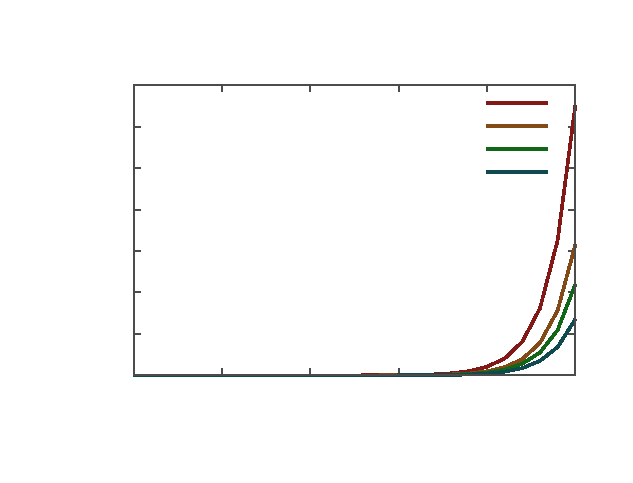
\includegraphics{./graficos/hanoi-linux-opt}}%
    \gplfronttext
  \end{picture}%
\endgroup

	\end{center}


\section*{Anexo}
\subsection*{Características de los ordenadores donde se ha compilado}


\end{document}

